\documentclass[./main.tex]{subfiles}
\graphicspath{{\subfix{./figs}}}

% ------------ main document ------------ 
\begin{document}

\chapter{\chapHydro} \label{chap:hydrology}

% custom paragraph skip
\setlength{\parskip}{0mm}

\epigraph{\small{A afirmação ou suposição de que todas as enchentes são causadas por enxurradas superficiais tem persistido em artigos e até mesmo em alguns livros-texto de hidrologia, apesar de muitas evidências em contrário nas pesquisas florestais e agrícolas.}}{Hewlett \& Hibbert (1967, p. 275) \cite{Hewlett1967}}

\epigraph{\small{Uma caixa, objetivamente definida por dinâmicas distintas de água subterrânea, química da solução do solo ou composição isotópica, com área, profundidade e porosidade definidas, é um bloco de modelagem muito melhor do que uma infinidade de elementos em paisagens que são notoriamente heterogêneas tanto vertical quanto lateralmente!}}{Jeffrey McDonnell (2003, p. 1872) \cite{Mcdonnell2003a}}


% custom paragraph skip
\setlength{\parskip}{\myparskip}

\section{Bacias de ordem zero} \label{sec:hydro:intro}

\par A \textbf{\gls{hydrology}} é a ciência que estuda as águas continentais, buscando entender como a água se distribui nos continentes depois de se precipitar da atmosfera e antes de retornar aos oceanos \cite{chow1964}. Em outras palavras, a \gls{hydrology} investiga como o \textbf{\gls{hydro_cicle}} se manifesta em sua fase terrestre, em contraste com a Meteorologia (que se foca na atmosfera) ou Oceanologia (que estuda os oceanos). Ao ponderar sobre isso, é fácil imaginar grandes rios, como o Amazonas e o Paraná, além de outros notáveis como o Danúbio, o Nilo, o Amarelo, o Indo, o Ganges e o Mississípi. No caso do Brasil, surgem imagens de uma natureza exuberante, incluindo as vastas várzeas amazônicas e pantaneiras, assim como as espetaculares cataratas do rio Iguaçu. Também emergem visões relacionadas à intervenção humana em larga escala, como o complexo hidrelétrico, com suas barragens espalhadas pelo País, e os grandes projetos de transposição e irrigação, exemplificados pelos reservatórios na Serra da Cantareira, a transposição do Rio São Francisco e os pivôs centrais na bacia do Rio São Marcos. As recentes inundações que devastaram as cidades localizadas nos vales fluviais do Rio Grande do Sul, ilustram também que os rios são cruciais não somente para a produção de energia e de alimentos, mas também para a garantia da saúde básica e segurança física dos habitantes de vastas metrópoles urbanas. Nessa linha, não é raro que livros didáticos de \gls{hydrology} mencionem como as primeiras cidades-estado, surgidas na Mesopotâmia e no Egito, desenvolveram uma relação quase que simbiótica com grandes rios e suas planícies inundáveis. Água e sociedade estão intimamente ligadas. 

\begin{figure}[t!] 
\centering				
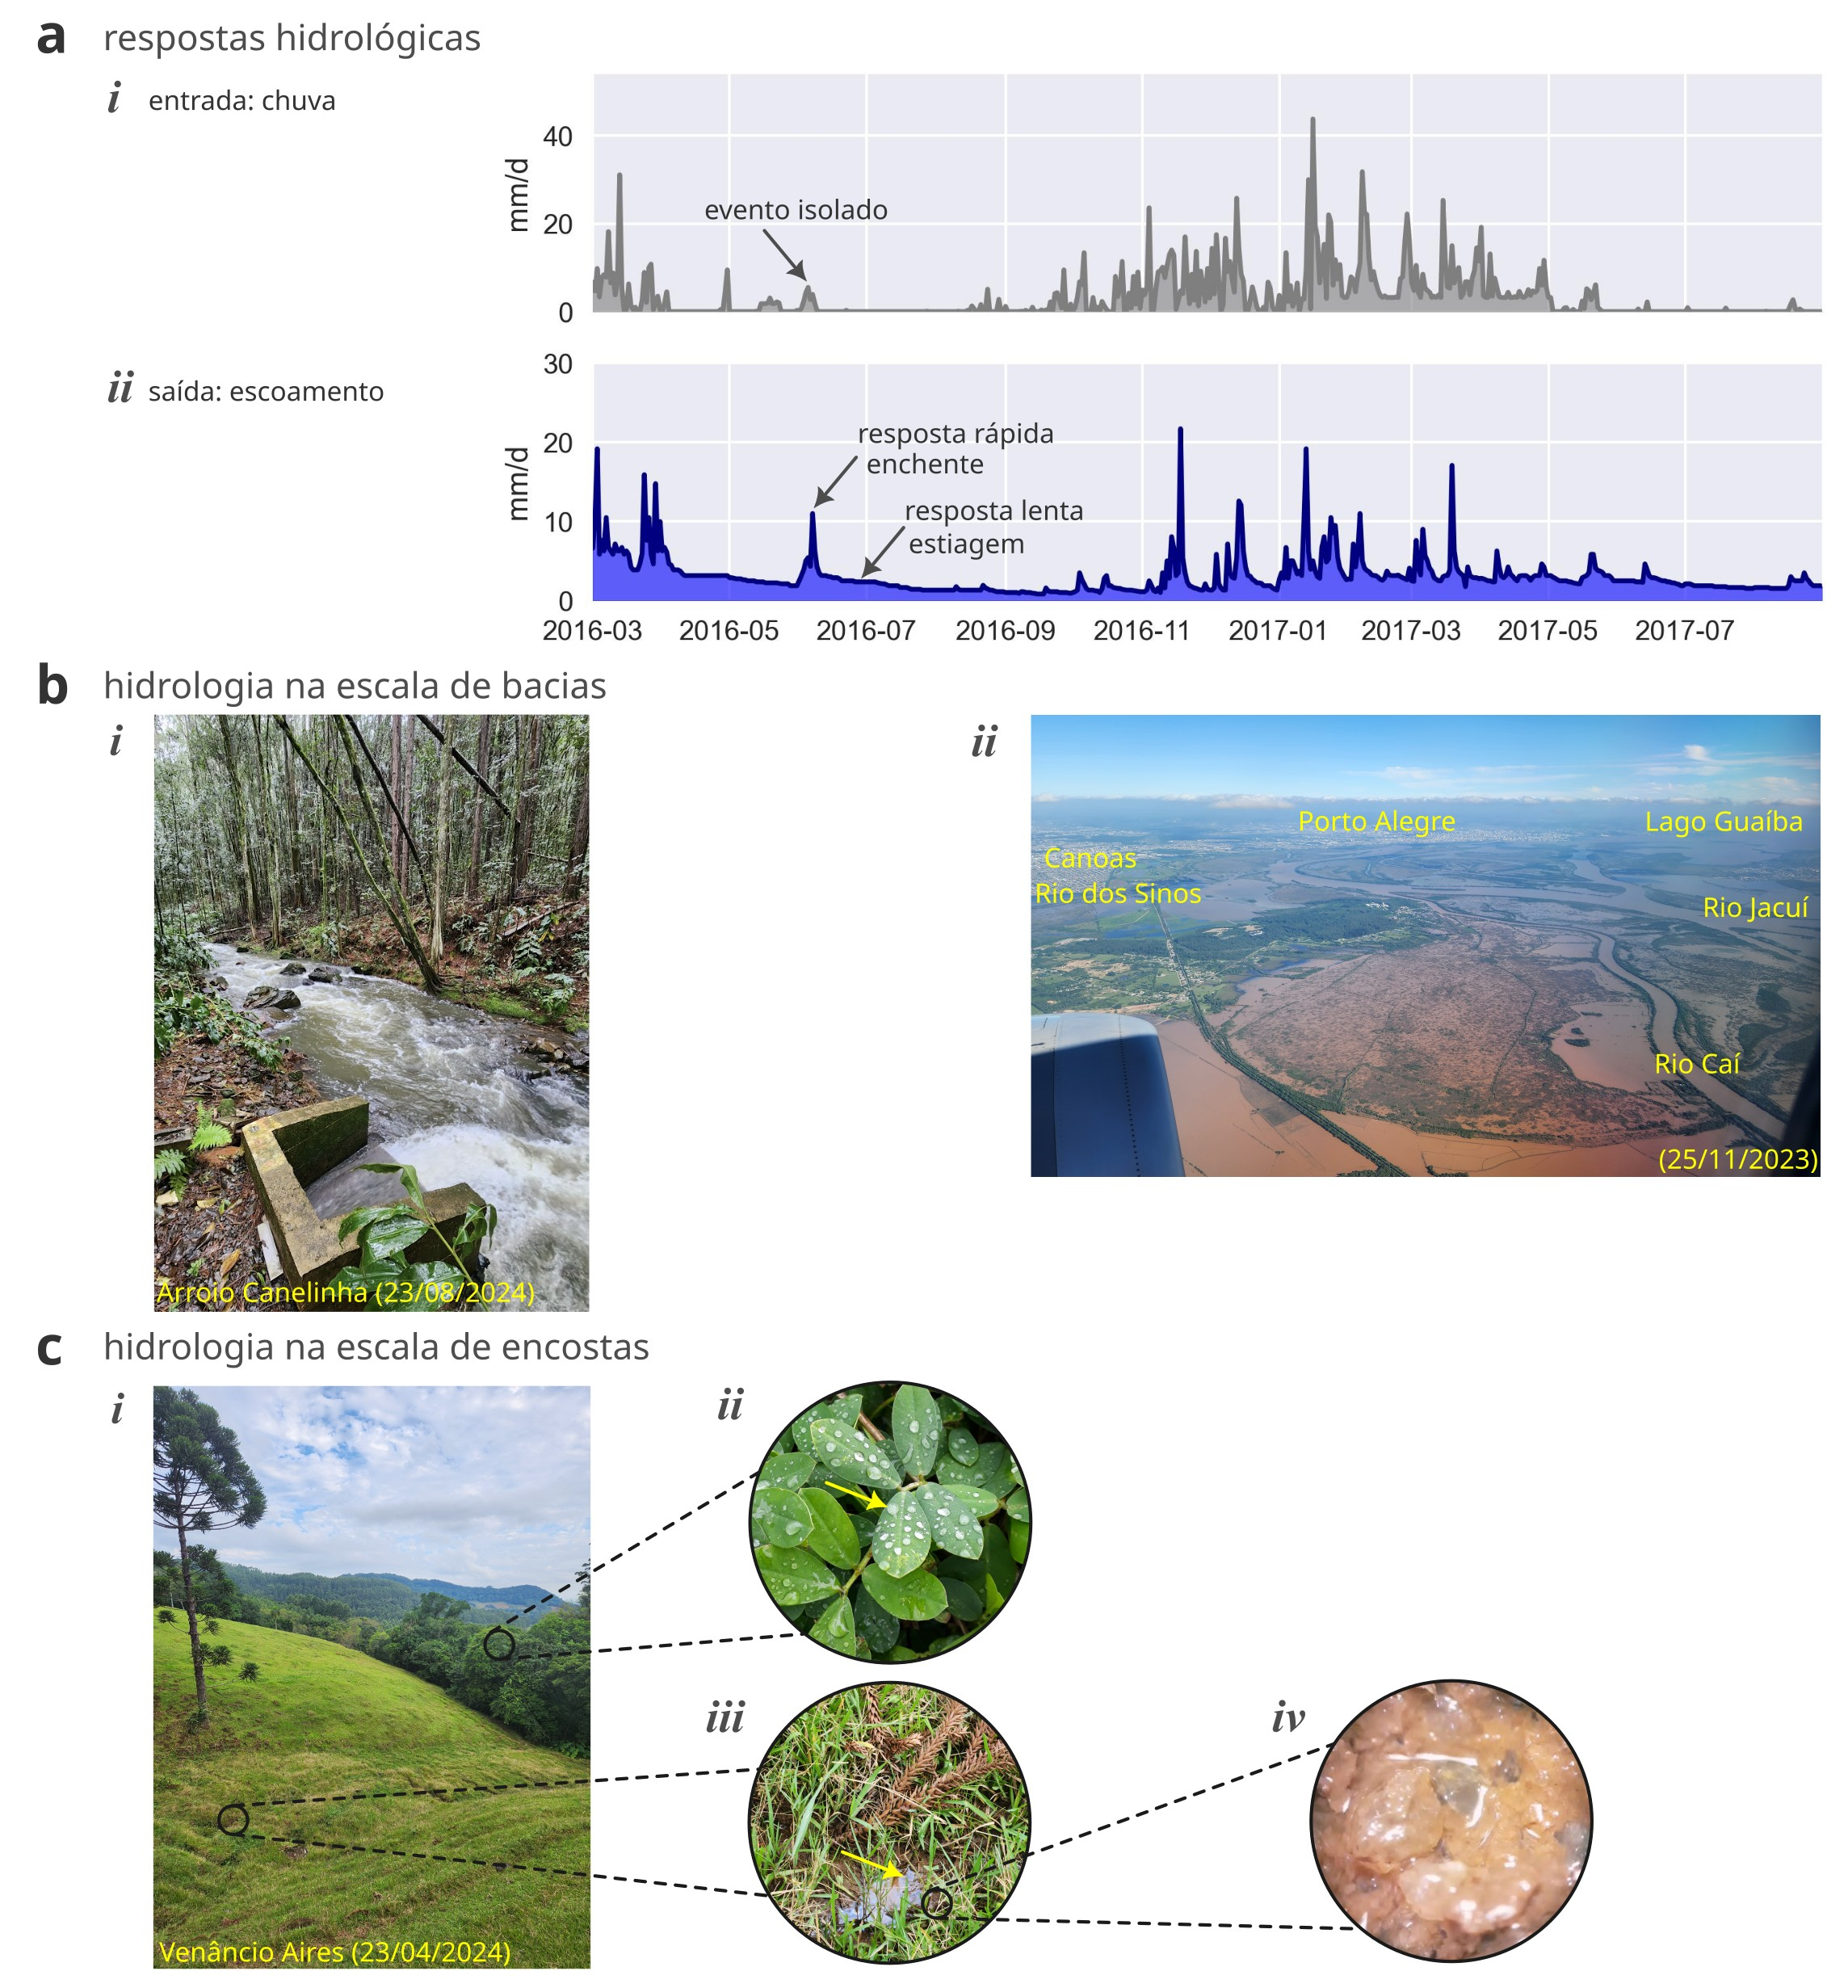
\includegraphics[width=0.98\linewidth]{figs/fig_zero.jpg}		
\caption[Encostas: onde tudo começa]
{\textbf{---\;Encostas: onde tudo começa.}
    A escala mais intuitiva quando se pensa em processos hidrológicos é o escoamento da água em rios, que são canais que drenam as águas para o oceano. Mas as respostas hidrológicas aos eventos de chuva originam-se nas encostas, nas bacias de ordem zero, onde a chuva interage com a paisagem.\;\textbf{a}\;---\;A alternância entre respostas rápidas (enchentes, detalhe \textrm{\textit{i}}) e respostas lentas (estiagens, detalhe \textrm{\textit{ii}}), observada em uma área de drenagem de médio porte na bacia Paraíba do Sul (342 km², Rio de Janeiro). Chuva diária obtida pela Estação \texttt{INMET 83738} (Resende) e vazão diária obtida pela Estação \texttt{ANA 58287000} (Rialto).\;\textbf{b}\;---\;Os processos hidrológicos evidentes na escala das bacias incluem a propagação do escoamento pela rede de drenagem, morro abaixo (detalhe \textrm{\textit{i}}) e as inundações das planícies, quando o escoamento dos rios extravasa a seção maior dos canais, invadindo os terrenos secos adjacentes (detalhe \textrm{\textit{ii}}).\;\textbf{c}\;---\;A água que abastece o escoamento dos rios advém da interação das chuvas com as encostas (detalhe \textrm{\textit{i}}), resultando em processos na superfície (como a \gls{interception}, no detalhe \textrm{\textit{ii}}) e abaixo da superfície (como a saturação do solo, detalhes \textrm{\textit{iii}} e \textrm{\textit{iv}}. 
}
\label{fig:hydro:intro} 		
\end{figure}

\par Essa interpretação intuitiva da \gls{hydrology}, no entanto, resulta de duas percepções particulares. A primeira delas é o \textbf{\gls{bias-engineer}} que permeia a \gls{hydrology}, que desde sempre é marcada por uma \textbf{\gls{dual-sci-mgmt}}. Essa dualidade implica que a \gls{hydrology} existe em uma interface fluida entre a investigação teórica sobre a natureza (problemas \textit{importantes} para o conhecimento humano) e a solução prática de impasses sociais, ambientais e econômicos (problemas \textit{urgentes} para as pessoas). James Dooge (1988) \cite{Dooge1988} sustenta que o campo nasceu de forma relativamente distinta de outras disciplinas científicas, como a Física ou Biologia, sendo essencialmente pragmática em sua formação. Ao longo da História, os problemas hidrológicos em geral se apresentavam diretamente de sua aplicação, para então novos dados serem obtidos e, por fim, algum conhecimento ser produzido. Como exemplo, Dooge ilustra que, de acordo com Plínio O Velho (24-79 DC), o nível do Rio Nilo era medido na Antiguidade não em termos de vazão, mas em uma escala do impacto socioeconômico implicado: fome (nível baixo), segurança (nível médio) e desastre (acima da cota de inundação). Nessa linha, Murugesu Sivapalan e Günter Blösch sugerem que o campo evoluiu de uma fase baseada em métodos de engenharia reducionistas e pragmáticos (Era Empírica), para tornar-se durante o século XX uma Ciência da Terra (Era da Geociência), holística e integradora, fundindo-se com ramos importantes da Geografia Física, Geologia, Pedologia, Ecologia e, recentemente, da Sociologia (Era da Co-evolução) \cite{Sivapalan2017, Sivapalan2018}. A segunda percepção é o \textbf{\gls{bias-fluvial}} que domina o campo, em especial em lugares atravessados por grandes rios, como é o caso do Brasil, dos Estados Unidos, da China e da Europa Central. Essa visão direciona os estudos hidrológicos para problemas essencialmente hidráulicos em escala continental, tais como a propagação de vazão nos canais da rede de drenagem, a inundação das planícies adjacentes e, com o advento do sensoriamento remoto, do balanço hídrico continental. A eficiência de atividades econômicas como a produção de energia elétrica, navegação, saneamento básico, irrigação, etc, dependem fundamentalmente desse tipo e conhecimento. Esse viés faz sentido em boa parte dos continentes, mas possui um peso menor em regiões dominadas por rios de pequeno e médio porte, como nos arquipélagos do Japão, da Nova Zelândia e nas Ilhas Britânicas. A perspectiva fluvialista é ilustrada pela impressão relatada por um hidrólogo brasileiro em uma visita ao Reino Unido:

\begin{adjustwidth}{100pt}{0pt}
\medskip
\small Quando eu estava na Inglaterra, fui conhecer uma certa estação fluviométrica de referência em um rio famoso na região. Falavam do tal rio o tempo todo, mas quando cheguei no local, fiquei um tanto perplexo e decepcionado. Aquilo não era um rio: era uma sanga. Com algum impulso, era possível até mesmo pular na outra margem. -- Walter Collischonn (2023, em comunicação pessoal).
\medskip
\end{adjustwidth}

\noindent Com a ação desses dois vieses, é um tanto fácil esquecer de que a água só escoa nos rios como consequência dos processos que ocorrem nas encostas dos morros e, em última instância, no perfil vertical que começa no dossel da vegetação, passa pela superfície e horizontes do solo e termina no embasamento subterrâneo de rocha. A propagação do escoamento pelos canais e as inundações de planícies nada mais são que processos de transporte e dissipação das enchentes produzidas pela interação das chuvas com o terreno mais alto e montanhoso da paisagem. Essa importância da \textit{escala da encosta} foi ressaltada inicialmente no Japão por Tsukamoto (1973) \cite{tsukamoto1973} no início dos anos 70, que ampliou a hierarquização sistemática de canais proposta por Strahler (1957) \cite{strahler1957} ao introduzir o conceito de \textbf{\gls{zero-basin}} (em japonês: \begin{CJK}{UTF8}{min}0 次 谷\end{CJK}). Ainda que a ênfase de Tsukamoto nas encostas e talvegues do terreno avance sobre questões específicas de erosão e produção de sedimentos, é evidente a sua importância primordial no \gls{hydro_cicle}. Como ilustrado na Figura \ref{fig:hydro:intro}, \textit{é nas bacias de ordem zero onde tudo começa}. A alternância entre enchentes e estiagens, observação primordial na \gls{hydrology} (Figura \ref{fig:hydro:intro}\textbf{a}), não se origina pela propagação da água rio abaixo, ou pela inundação de planícies (Figura \ref{fig:hydro:intro}\textbf{b}), mas pela interação das chuvas com a paisagem, na escala das encostas (Figura \ref{fig:hydro:intro}\textbf{c}). Nessa mesma linha, Mediondo \& Tucci (1997) \cite{mediondo1997} utilizam o termo \textbf{bacia de vertente}, que eles também defendem ser o ponto de partida para entender a diversidade de processos hidrológicos, com reflexos tanto na micro quanto na macroescala. Utilizarei aqui o termo \gls{zero-basin}, considerando que, de acordo com Godoy et \textit{al.} (2021) \cite{godoy2021}, esse termo se popularizou na literatura internacional.

\par A Tabela \ref{tbl:processes} organiza a nomenclatura sobre os processos hidrológicos que ocorrem nas encostas e talvegues do terreno, a serem explorados com mais detalhe neste capítulo. Ainda que relevantes na \gls{teoria}, seria essa diversidade toda relevante \textit{na prática}? Ao se considerar a aplicação de modelos hidrológicos para ajudar na tomada de decisão e formulação de estratégias de alavancagem, o quanto a complexidade que existe nas bacias de ordem zero pode ser simplificada ou mesmo negligenciada? Afinal, como vimos no Capítulo \ref{chap:systems}, a modelagem de sistemas precisa fazer uso de idealizações, que são simplificações deliberadas para tornar o \gls{sys-target} mais palpável. Além disso, diante de rios que percorrem distâncias continentais, os detalhes mínimos sobre os processos hidrológicos nas bacias de ordem zero acabam por perder qualquer sentido prático. A mera confluência de dois rios de médio porte ou uma inundação de planície pode apagar completamente a assinatura hidrológica deixada por alguma característica típica produzida pelos processos nas encostas. A massa de água e de sedimentos, energia e momento necessariamente se preservam pelas leis da conservação, mas informações detalhadas são progressivamente atenuadas e misturadas no grande caudal que se desloca para o oceano. Nesse sentido, desde que um \gls{model} apresente resultados quantitativos empiricamente adequados, os detalhes sobre os processos nas bacias de ordem zero seriam irrelevantes.

\par Esse \textit{apelo para a simplificação} torna-se uma objeção sedutora, pois facilita em grande medida o processo de modelagem. Mas ele é apenas um reflexo do \gls{bias-fluvial}: uma perspectiva que enquadra questões a serem compreendidas e problemas a serem resolvidos de montante para jusante, rio abaixo. Nessa linha, os modelos hidrológicos mais populares, ao menos no Brasil, como \texttt{SWAT}, \texttt{HEC-HMS}, \texttt{MGB}, \texttt{SWMM}, tratam as bacias de ordem zero como unidades herméticas, ou caixas-pretas, sendo impossível recuperar detalhes sobre os processos hidrológicos nas encostas e talvegues do terreno, a não ser em termos médios e agregados. No final das simulações computacionais, a visualização mais informativa possível é um mosaico de sub-bacias\footnote{Também é possível recuperar informações nas unidades de \gls{hydro-response} internas a cada sub-bacia. No entanto, como veremos adiante, essa representação é irremediavelmente estática, ao passo que os processos na escala de bacias de ordem zero são dinâmicos no tempo e no espaço.}. É claro que essa simplificação se justifica quando o objetivo de um dado estudo é compreender fenômenos e resolver problemas hidrológicos de jusante, ou seja, fluviais. Porém, para endereçar boa parte dos problemas relacionados com a segurança hídrica, como a revitalização de bacias hidrográficas, é necessário assumir um olhar de jusante para montante, encosta acima, representando com detalhes suficientes as bacias de ordem zero, pois é nessa escala que os processos relevantes acontecem e ações precisam ser especificadas. Para tanto, um \gls{model} útil deve levar suficientemente a sério o que as teorias hidrológicas dizem sobre a geração de escoamento em bacias de ordem zero. Do contrário, corre-se o risco de se instanciar um \gls{model} que não passa tanto no teste da adequação da fronteira quanto no teste da adequação da estrutura (ver Seção \ref{sec:sys:diags}). 

\par Dito isso, este capítulo marca o ponto em que passarei a articular como as teorias sobre as respostas hidrológicas em bacias de ordem zero podem ser veiculadas por modelos hidrológicos. Esse é um ponto crítico, pois aqui encontraremos todos os desafios e problemas filosóficos, científicos e técnicos expostos nos dois capítulos anteriores, mas agora sob um enfoque hidrológico. Os tópicos serão todos revisitados direta ou indiretamente, tais como a ascensão e queda de paradigmas, a refutação e confirmação de hipóteses, os problemas de estrutura, dimensionalidade e subdeterminação, etc. Em essência, se verá que a complexidade dos processos hidrológicos no solo e nas encostas trazidas por evidências empíricas, somada com a dificuldade de se obter observações diretas em uma bacia qualquer, torna qualquer tentativa de modelagem alicerçada em formalizações matemáticas contínuas e distribuídas no espaço um esforço desproporcional. Como veremos, uma solução unificadora para esse problema, proposta recentemente por Jeffrey McDonnell (2021) \cite{mcdonnell2021}, consiste em adotar modelos conceituais que representam \textit{efetivamente} os processos de \textbf{conectividade} na escala que precisamos endereçar para responder nossas perguntas de pesquisa. Voltando à \gls{analogy} da paisagem que introduzi no início desta tese, claramente estamos saindo dos vales estreitos de assuntos abstratos e filosóficos para adentrar em um campo mais aberto, de questões mais tangíveis e aplicadas. Aqui, os riachos das montanhas se unem, formando rios caudalosos que fluem por barras e barrancas.

{\renewcommand{\arraystretch}{1.5}% for the vertical padding
\begin{table}[t!]
    \centering	
    \tiny
    \sffamily
    \rowcolors{2}{white}{rowgray}
    \begin{tabular}{ 
        >{\raggedright\arraybackslash}m{1cm}  
        >{\raggedright\arraybackslash}m{6cm}  
        >{\raggedright\arraybackslash}m{1cm}
        >{\raggedright\arraybackslash}m{1cm}
        >{\raggedright\arraybackslash}m{2cm}}
        \toprule
        \textbf{Componente} & \textbf{Nome} & \textbf{Dimensão} & \textbf{Unidade} & \textbf{Categoria} \\ 
        \midrule
        
        $\textbf{C}$ & dossel da vegetação & L & mm & reservatório \\ 
        $\textbf{S}$ & superfície do solo & L & mm & reservatório \\ 
        $\textbf{O}$ & horizonte orgânico & L & mm & reservatório \\ 
        $\textbf{V}$ & zona vadosa, horizonte mineral & L & mm & reservatório \\
        $\textbf{V}_{\text{c}}$ & água capilar na zona vadosa & L & mm & reservatório \\
        $\textbf{V}_{\text{g}}$ & água gravitacional na zona vadosa & L & mm & reservatório \\
        $\textbf{D}_\text{v}$ & déficit capilar & L & mm & reservatório \\
        $\textbf{G}$ & zona freática & L & mm & reservatório \\
        $\textbf{D}$ & déficit de saturação & L & mm & reservatório \\
        
        $p$ & precipitação, chuva & L/T & mm/h & fluxo (exógeno)\\
        $p_{\text{s}}$ & chuva efetiva & L/T & mm/h & fluxo\\
        $p_{\text{x}}$ & chuva excedente & L/T & mm/h & fluxo\\
        
        $Q$ & vazão no rio, escoamento fluvial & L$^{3}$/T & l/h & fluxo\\
        $q$ & vazão específica no rio, escoamento fluvial & L/T & mm/h & fluxo\\
        
        $f$ & infiltração & L/T & mm/h & fluxo\\        
        $q_{\text{si}}$ & enxurrada, \gls{rie} & L/T & mm/h & fluxo\\
        $q_{\text{se}}$ & chuva direta, escoamento superficial por excesso de saturação & L/T & mm/h & fluxo\\
        $q_{\text{ss}}$ & exfiltração, escoamento subsuperficial, escoamento lateral & L/T & mm/h & fluxo\\
        $q_{\text{o}}$ & percolação entre horizontes & L/T & mm/h & fluxo\\
        $q_{\text{v}}$ & recarga, percolação final & L/T & mm/h & fluxo\\
        $Q_{\text{g}}$ & escoamento de base, afloramento subterrâneo lento & L$^{3}$/T & l/h & fluxo\\
        $Q_{\text{gt}}$ & escoamento translacional, afloramento subterrâneo rápido & L$^{3}$/T & l/h & fluxo\\ 
        
        $e_{\text{pot}}$ & \acrlong{et} potencial & L/T & mm/h & fluxo (exógeno)\\
        $e_{\text{c}}$ & evaporação no dossel & L/T & mm/h & fluxo\\
        $e_{\text{s}}$ & evaporação na superfície & L/T & mm/h & fluxo\\
        $e_{\text{o}}$ & transpiração no horizonte orgânico & L/T & mm/h & fluxo\\
        $e_{\text{v}}$ & transpiração na zona vadosa & L/T & mm/h & fluxo\\
        $e_{\text{g}}$ & transpiração na zona freática & L/T & mm/h & fluxo\\
        
        $f_\text{max}$ & capacidade de infiltração & L/T & mm/h & parâmetro \\ 
        $K$ & condutividade hidráulica & L/T & mm/h & parâmetro \\ 
        $g$ & tempo de detenção do aquífero & T & h & parâmetro \\ 
        $c_\text{max}$ & capacidade de \gls{interception} & L & mm & parâmetro \\ 
        $s_\text{max}$ & capacidade de detenção superficial & L & mm & parâmetro \\ 
        $o_\text{max}$ & capacidade de campo do horizonte orgânico & L & mm & parâmetro \\
        $v_\text{max}$ & capacidade de campo do horizonte mineral & L & mm & parâmetro \\
        $m$ & constante de uniformidade vertical do solo & L & mm & parâmetro \\

        
        \bottomrule
    \end{tabular}
    \caption[Processos hidrológicos em bacias de ordem zero]{\textbf{Processos hidrológicos em bacias de ordem zero} --- Relação de reservatórios, fluxos e \gls{parameters} globais dos processos hidrológicos em bacias de ordem zero. 
    }
    \label{tbl:processes}
\end{table} 
}

\section{Infiltração} \label{sec:hydro:mechs}

\begin{figure}[t!] 
\centering				
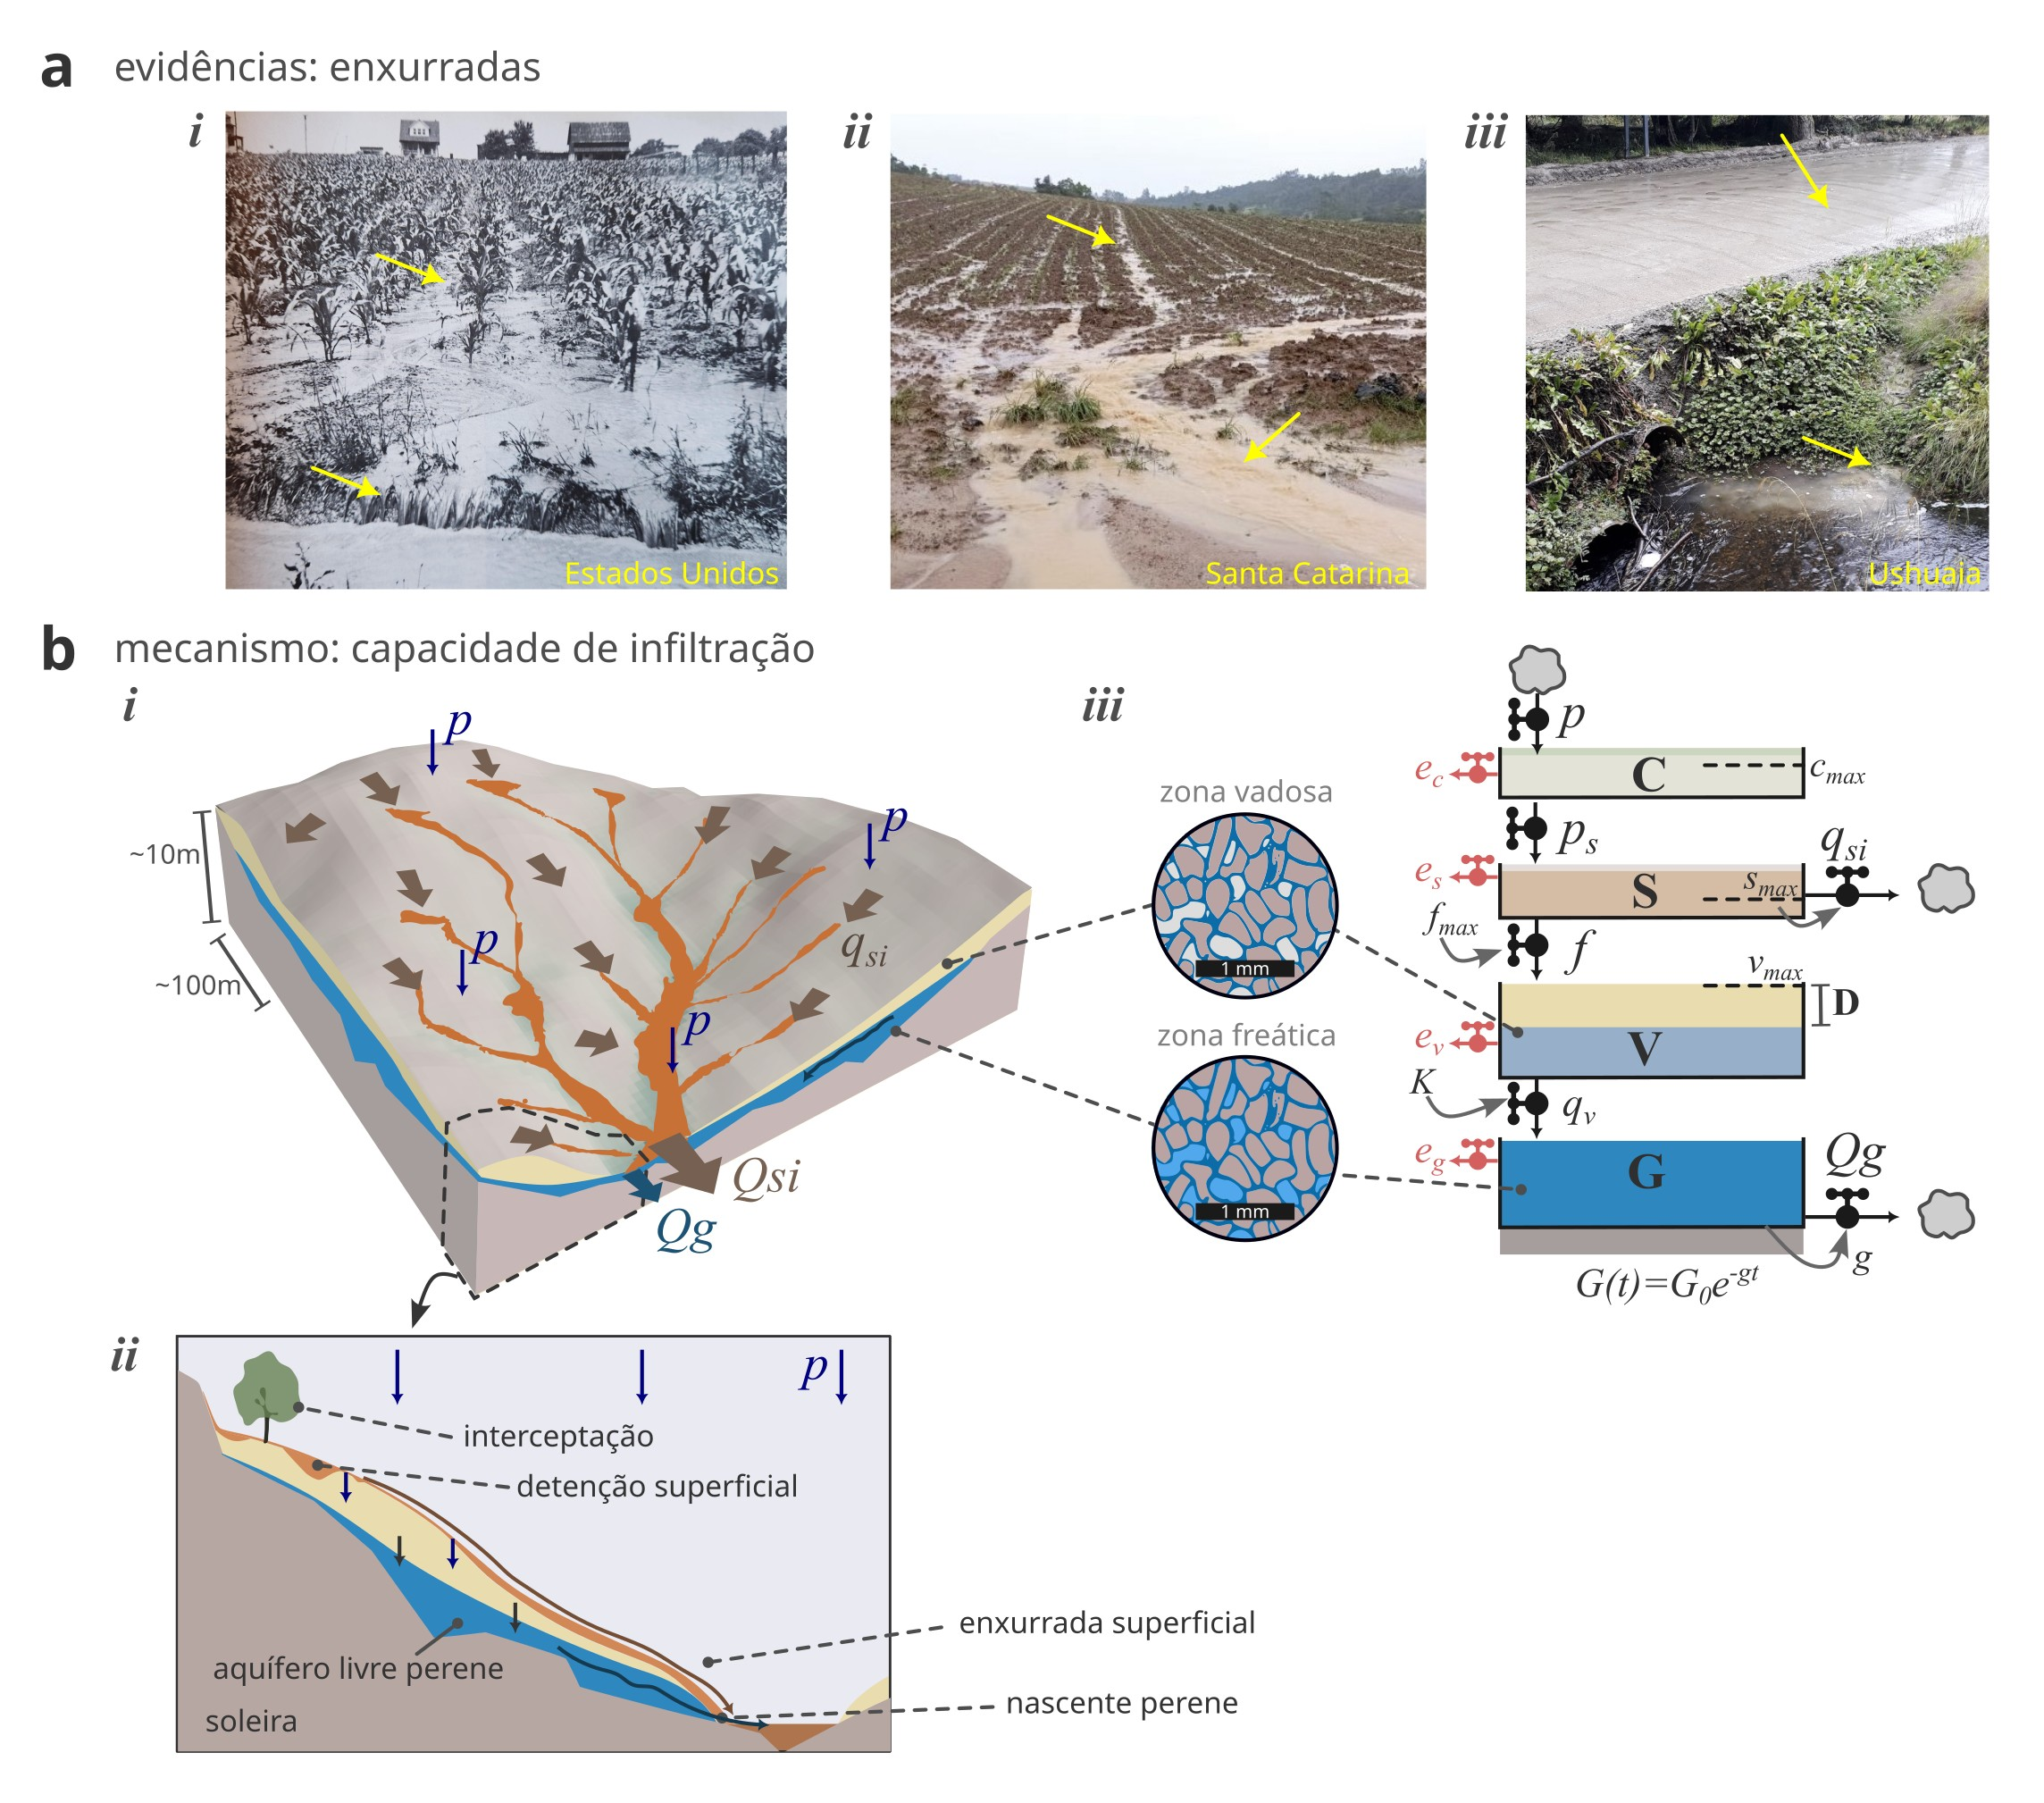
\includegraphics[width=0.98\linewidth]{figs/fig_horton.jpg}		
\caption[O \gls{paradigma} Hortoniano]
{
\textbf{---\;O \gls{paradigma} Hortoniano.} O \gls{paradigma} Hortoniano explica a alternância entre enchentes e estiagens com base no conceito da \gls{infmax} do solo.\;\textbf{a}\;---\;As evidências empíricas motivadoras são as enxurradas superficiais observadas após as chuvas, quando a água não consegue se infiltrar: enxurrada nos Estados Unidos reportada pelo \acrshort{scs} \cite{strahler1986} (detalhe \textrm{\textit{i}}); enxurrada em Santa Catarina reportada pela \texttt{EPAGRI} \cite{epagri2024} (detalhe \textrm{\textit{ii}}), e; enxurrada de estrada rural em Ushuaia, de autoria própria (detalhe \textrm{\textit{iii}}).\;\textbf{b}\;---\;A \gls{sf-runoff} ocorre de forma generalizada na bacia (detalhe \textrm{\textit{i}}) a partir do momento em que o fluxo de chuva supera a \gls{intercep-capacity} e a \gls{sfmax} (detalhes \textrm{\textit{ii}} e \textrm{\textit{iii}}).
}
\label{fig:hydro:horton} 		
\end{figure}

\par Na Seção \ref{sec:systems:model} do capítulo anterior, organizei um protótipo de \gls{model} hidrológico objetivando ilustrar e articular como que a \gls{sys-dyn} pode ser empregada no processo de modelagem. O \gls{concept-model} obtido, mantido em uma condição minimalista, foi construído principalmente com base na percepção de que uma bacia hidrográfica apresenta \textbf{respostas rápidas e lentas} diante dos eventos de chuva, produzindo assim o fenômeno da alternância entre as \textbf{enchentes} e as \textbf{estiagens} nos rios \cite{Hewlett1967}. Essa é uma percepção fundamental na \gls{hydrology}: quando chove, os rios ficam agitados, a água fica mais turva, os níveis sobem (resposta rápida); entre uma chuva e outra, os rios se acalmam, a água fica mais limpa, os níveis descem (resposta lenta); se demorar muito tempo para chover de novo, os riachos menores começam a secar (o \gls{system} tende a se esvaziar). Com algum rigor empírico, esse fenômeno em uma bacia hidrográfica qualquer pode ser medido e reproduzido em gráficos com o suporte de um pluviômetro e uma régua de nível. Com um pouco mais de rigor empírico, a percepção desse fenômeno fica mais apurada ao se fazer expedições de campo, observando a dinâmica espacial e temporal das nascentes e charcos (de onde a água subterrânea aflora lentamente) e das enxurradas rápidas (causadas pelas chuvas mais intensas). 

\par No contexto de bacias de ordem zero, a \gls{teoria} científica dominante hoje postula que as respostas hidrológicas aos eventos de chuva são a consequência de \textbf{múltiplos mecanismos de geração de escoamento}, superficiais e subterrâneos, tanto rápidos quanto lentos, simultâneos ou não, que serão descritos na próxima seção. Esses mecanismos foram revelados e corroborados por sucessivas investigações experimentais em pequenas bacias, encostas com trincheiras e parcelas de solo durante uma revolução científica na \gls{hydrology}, que ocorreu ao longo da segunda metade do século XX. Antes dessa revolução, contudo, a explicação científica hegemônica para as respostas rápidas e lentas das encostas era baseada principalmente na \gls{teoria} hidrológica de Robert Horton (1875-1945) \cite{Horton1933, Beven2004a}. Uma vez publicado, o \gls{percept-model} descrito por Horton consolidou-se como um verdadeiro \gls{paradigma} nos anos e décadas subsequentes, demarcando a chamada \textbf{\gls{age_inf}} -- um longo período de \gls{ciencia-normal} em que a \gls{comunidade-cientifica} desenvolveu pesquisas em frentes puras e aplicadas para articular as suas implicações \cite{Cook1946, Beven2021b}. Ainda que finalmente suplantada por uma explicação mais complexa, a \gls{teoria} de Horton, por ser científica (isto é, falseável), contribuiu sobremaneira em elevar a \gls{hydrology} de sua Era Empírica, focada em aplicações de engenharia, para ser entendida como uma Geociência, focada em explicar os fenômenos da natureza.

\par A ideia central do \gls{percept-model} de Horton é estabelecida no artigo \textit{O papel da infiltração no ciclo hidrológico}\footnote{Tradução livre de: \textit{The role of infiltration in the hydrological cycle}} (1933) \cite{Horton1933}, em que o solo é concebido como uma \textit{superfície separadora} da chuva: uma parte da água da chuva se infiltra nas encostas, alojando-se na matriz do solo, e outra parte escoa superficialmente em \textbf{enxurradas}, causando aumentos dramáticos na vazão dos rios, morro abaixo (Figura \ref{fig:hydro:horton}\textbf{a}). A \textbf{\gls{infiltration}}, assim, consistiria no processo-chave para se compreender o \gls{hydro_cicle} na sua fase terrestre:

\begin{adjustwidth}{100pt}{0pt}
\medskip
\small A infiltração divide a precipitação em duas partes, que posteriormente seguem caminhos diferentes através do \gls{hydro_cicle}. Uma parte segue através da \gls{sf-runoff} e dos canais dos rios até o oceano como escoamento fluvial; a outra parte vai inicialmente para o solo e daí através do fluxo de água subterrânea novamente para o rio ou é devolvida para o ar por processos evaporativos. Portanto, o solo atua como uma superfície separadora, e o autor acredita que vários problemas hidrológicos são simplificados ao começar por essa superfície e seguir o curso subsequente de cada parte da precipitação assim dividida, separadamente.\footnote{Tradução livre de: \textit{Infiltration divides rainfall into two parts, which thereafter pursue different courses through the hydrologic cycle. One part goes via overland flow and stream-channels to the sea as surface-runoff; the other goes initially into the soil and thence through ground-water flow again to the stream or else is returned to the air by evaporative processes. The soil therefore acts as a separating surface, and the author believes that various hydrologic problems are simplified by starting at this surface and pursuing the subsequent course of each part of the rainfall as so divided, separately.}} -- Robert Horton (1933, p. 446–447) \cite{Horton1933}. 
\medskip
\end{adjustwidth}

\par Para articular esse \gls{percept-model}, Horton instancia diversos fluxos, reservatórios e \gls{parameters} importantes do \gls{system} que representa a \gls{zero-basin}. A Figura \ref{fig:hydro:horton}\textbf{b}, ilustra o \gls{system} modelado (os fluxos de evapotranspiração em cada reservatório são denotados por $E$). O fluxo primordial consiste na \textbf{\gls{ground-rain}}\footnote{Tradução livre de \textit{ground-rainfall.}}, ou seja, o fluxo da chuva que de fato atinge o solo após a chuva $p$ superar a \gls{intercep-capacity} no \gls{canopy}. O solo, por sua vez, consiste em uma matriz porosa de minerais sólidos que armazena água em filmes mantidos pela tensão superficial de suas partículas, formando assim a \textbf{\gls{unsat-zone}}\footnote{Tradução livre de \textit{unsaturated zone}.}. acreção de água nos filmes nessa zona ocorre até um certo limite, que é a \textbf{\gls{fmc}}\footnote{Tradução livre de \textit{field moisture-capacity}} característica do solo. Essa água na \gls{unsat-zone}, que está presa aos poros, é denominada \textbf{\gls{water_capilar}}. Além da \gls{fmc}, os filmes de água nas partículas, ao se mesclarem, criam uma massa de água relativamente móvel, denominada de \textbf{\gls{water_gravit}}. Essa água, então, percola verticalmente através dos poros pela ação da gravidade, formando uma \textbf{\gls{sat-zone}} sobre a soleira impermeável, que é o embasamento de rocha sã (ou seja, essa zona forma um aquífero livre). Horton denomina de \textbf{\gls{qv}}\footnote{Tradução livre de \textit{re-charge}.}, ou \textit{percolação última}, o fluxo vertical de água da suspensa na \gls{unsat-zone} para o aquífero da \gls{sat-zone}, processo que pode eventualmente aumentar o nível do lençol freático (aumentando, portanto, a carga hidráulica nesse \gls{system} poroso). Nessa linha, o \textbf{\gls{dgrav}} consiste na quantidade de \gls{water_gravit} na \gls{unsat-zone} necessária para se atingir a completa saturação do solo e, por consequência, o afloramento do lençol freático na superfície\footnote{O \gls{dgrav} pode ser também interpretado como a capacidade gravitacional da zona vadosa, ou ainda a profundidade efetiva do lençol freático.}. Aqui, o \gls{flux-max} da \gls{qv} é limitado pela \textbf{\gls{cond-hyd}} do solo: quanto mais próximo da saturação encostra-se a \gls{unsat-zone}, a percolação vertical tende a ser dominada pela carga hidráulica, vencendo a tensão superficial.

\par Nesse ponto, Horton apresenta um parâmetro crucial em seu \gls{percept-model}: a \textbf{\gls{infmax}}, isto é, o \gls{flux-max} possível de infiltração que a superfície do solo oferece em um dado momento. É importante destacar que essa capacidade é um atributo da fina camada superficial do solo e, de acordo com Horton, tende a ser inferior à \gls{cond-hyd} da matriz do solo, funcionando como um fator limitante crítico no \gls{system}. Dessa forma, a água de uma \gls{ground-rain} com intensidade menor ou igual à \gls{infmax} é completamente absorvida pela matriz do solo. Por outro lado, quando uma \gls{ground-rain} apresenta intensidade maior que a \gls{infmax}, então a água da \textbf{\gls{ex-rain}}\footnote{Tradução livre de \textit{rainfall-excess}.} passa a preencher as pequenas depressões superficiais. Se a \gls{ex-rain} persistir por tempo suficiente, a \textbf{\gls{sfmax}}\footnote{Tradução livre de \textit{detention-storage}.} é superada, e então se inicia o processo de \gls{sf-runoff}, ou \textbf{\gls{rie}}\footnote{Essa nomenclatura objetiva evitar confusões futuras, ainda que o termo original de Horton seja simplesmente \say{escoamento superficial} (\textit{surface-runoff}).}, onde a água da chuva escoa pelos sulcos e ravinas morro abaixo até atingir os canais dos riachos. 

\par A \gls{infmax} depende do tipo de solo, de sua textura e das práticas de manejo empregadas, o que implica em uma variabilidade na resposta de diferentes bacias, mesmo quando submetidas a eventos de chuva idênticos. Além da variabilidade espacial, Horton argumenta que a \gls{infmax} do solo varia ao longo do tempo, oscilando dinamicamente entre extremos da capacidade mínima e máxima, em um \textbf{ciclo de decaimento e restauração} (Figura \ref{fig:hydro:horton2}\textbf{a}). Nesse ciclo, a fase de decaimento ocorre durante os eventos de chuva em função da expansão de partículas coloidais, da colmatação por partículas finas e da compressão causada pelo impacto das gotas de chuva. Por outro lado, a fase de restauração ocorre durante os períodos de tempo seco, à medida que se abrem novas fissuras e poros pela retração das partículas coloidais, dilatações por diferenças de temperatura e pela atividade da fauna do solo, como insetos e minhocas. Com essa concepção, espera-se que uma chuva longa, mesmo que de relativa baixa intensidade, eventualmente produza \gls{sf-runoff} se o decaimento em curso levar a \gls{infmax} do solo para um valor \textit{abaixo} da intensidade da \gls{ground-rain}. Além disso, esse conceito introduz o efeito das \textbf{\gls{amc}}, como a diferença nas respostas entre o início e o final de uma estação chuvosa ou durante a entrada de uma frente fria com chuvas persistentes. Nesse caso, e se a velocidade de restauração da \gls{infmax} do solo for relativamente lenta, as chuvas subsequentes, mesmo que \textit{menos} intensas, tendem a produzir \textit{mais} \gls{sf-runoff} do que as chuvas iniciais. Em outras palavras, o comportamento do \gls{system} torna-se altamente não-linear.

\par Com a \gls{teoria} sobre o papel da infiltração no \gls{hydro_cicle}, Horton então avança para explicar definitivamente o fenômeno das enchentes\footnote{Tradução livre de \textit{stream rises}.} observada nos rios, propondo um método de separação do hidrograma (Figura \ref{fig:hydro:horton2}\textbf{b}). Com esse objetivo, ele sustenta que o escoamento fluvial\footnote{Tradução livre de \textit{total runoff}.} consiste em duas componentes de fluxo separáveis: (1) o fluxo de água subterrânea\footnote{Tradução livre de \textit{ground-water runoff}.}, que é uma resposta lenta do afloramento do aquífero livre, e; (2) o fluxo do escoamento superficial\footnote{Tradução livre de \textit{surface-runoff}.}, que é uma resposta rápida das enxurradas produzidas nas encostas. As duas respostas são controladas, em todo ou em parte, pela \gls{infmax} do solo:

\begin{adjustwidth}{100pt}{0pt}
\medskip
\small De acordo com esta \gls{teoria}, o escoamento fluvial total consiste em duas partes: (1) Escoamento superficial, que depende da quantidade de precipitação, da intensidade da chuva e da \gls{infmax} e é praticamente independente da taxa de evaporação. (2) Escoamento de água subterrânea. Este depende de (a) infiltração total e, portanto, indiretamente dos mesmos fatores que controlam a \gls{sf-runoff} e também depende de (b) atividade vegetal e evaporação, que em parte determinam as perdas de água, e de (c) as complexas inter-relações entre \gls{infmax}, \gls{fmc} do solo, atividade vegetal e \gls{qv} do aquífero.\footnote{Tradução livre de: \textit{In accordance with this theory, total runoff consists of two parts: (1) Suface-runoff, which is dependent on rainfall-amount, rain-intensity, and infiltration-capacity and is practically independent of evaporation-rate. (2) Ground-water runoff. This is dependent on (a) total infiltration and hence indirecty on the same factors which control surface-runoff and is also dependent on (b) vegetational activity and evaporation, which in part determine the water losses, and on (c) the complex interrelations between infiltration-capacity, field moisture-capacity, vegetational activity, and accretion to the water-table.}} -- Robert Horton (1933, p. 454) \cite{Horton1933}.
\medskip
\end{adjustwidth}

\noindent Assumindo que a \gls{sat-zone}, o aquífero livre, funciona como um \gls{linear-reserv}, a \textbf{\gls{deple-curve}}\footnote{Tradução livre de \textit{normal depletion curve}.} do \gls{ground-flow}, ou fluxo de afloramento, consiste em uma típica \gls{curve-exp-dec} do tipo $Q_{g} = Q_{g, o} e^{-t/g}$. Essa curva é uma característica física e o \gls{g-coef} pode ser extraído de hidrogramas durante os períodos de estiagem nos quais as perdas de água por evapotranspiração são mínimas (por exemplo, nos meses mais frios em locais de clima temperado e subtropicais). Uma vez obtida, a \gls{deple-curve} pode ser deslocada horizontalmente no hidrograma, permitindo-se separar a componente superficial da vazão fluvial da contribuição puramente subterrânea. Com isso, Horton propõe que existem quatro  tipologias possíveis de \gls{hydro-response} diante dos eventos de chuva. A resposta \textbf{Tipo 0} ocorre quando a intensidade da \gls{ground-rain} é inferior à \gls{infmax} e o total de água infiltrada é inferior ao \gls{fmd} (\textit{não} há \gls{sf-runoff} e \textit{não} há recarga). Nessa situação, mesmo que tenha chovido, não há mudança detectável na \gls{deple-curve} do rio. A resposta \textbf{Tipo 1}, por sua vez, ocorre quando a intensidade da \gls{ground-rain} é inferior à \gls{infmax}, mas o total de água infiltrada é superior ao \gls{fmd} (\textit{não} há \gls{sf-runoff} mas \textit{ocorre} \gls{qv} do aquífero). Nesse caso, a \gls{deple-curve} é deslocada, dependendo de quanto a \gls{qv} é superior (ou inferior) ao fluxo de afloramento, podendo inclusive produzir um pulso (relativamente lento) na vazão do rio puramente pelo aumento da carga hidráulica no \gls{system} aquífero. A resposta \textbf{Tipo 2} ocorre quando a intensidade da \gls{ground-rain} é superior à \gls{infmax} e o total infiltrado é muito baixo, inferior ao \gls{fmd} (\textit{ocorre} \gls{sf-runoff} mas \textit{não} ocorre \gls{qv} do aquífero). Esse tipo de resposta consiste em um pulso rápido de água da enxurrada superficial sobreposto à \gls{deple-curve} que se desenvolvia antes do evento. Por fim, a resposta \textbf{Tipo 3} acontece quando as duas respostas, rápida e lenta, ocorrem simultaneamente: tanto a \gls{sf-runoff} quanto a \gls{qv} do aquífero se manifestam na forma de pulsos sobrepostos. Essas quatro tipologias ilustram a complexidade que emerge a partir do \gls{percept-model} de Horton, proporcionando grande margem para explicações sobre as enchentes, que variam de acordo com as características da superfície, do solo, do subsolo, das chuvas e das condições antecedentes de umidade.

% figure
\begin{figure}[t!] 
\centering				
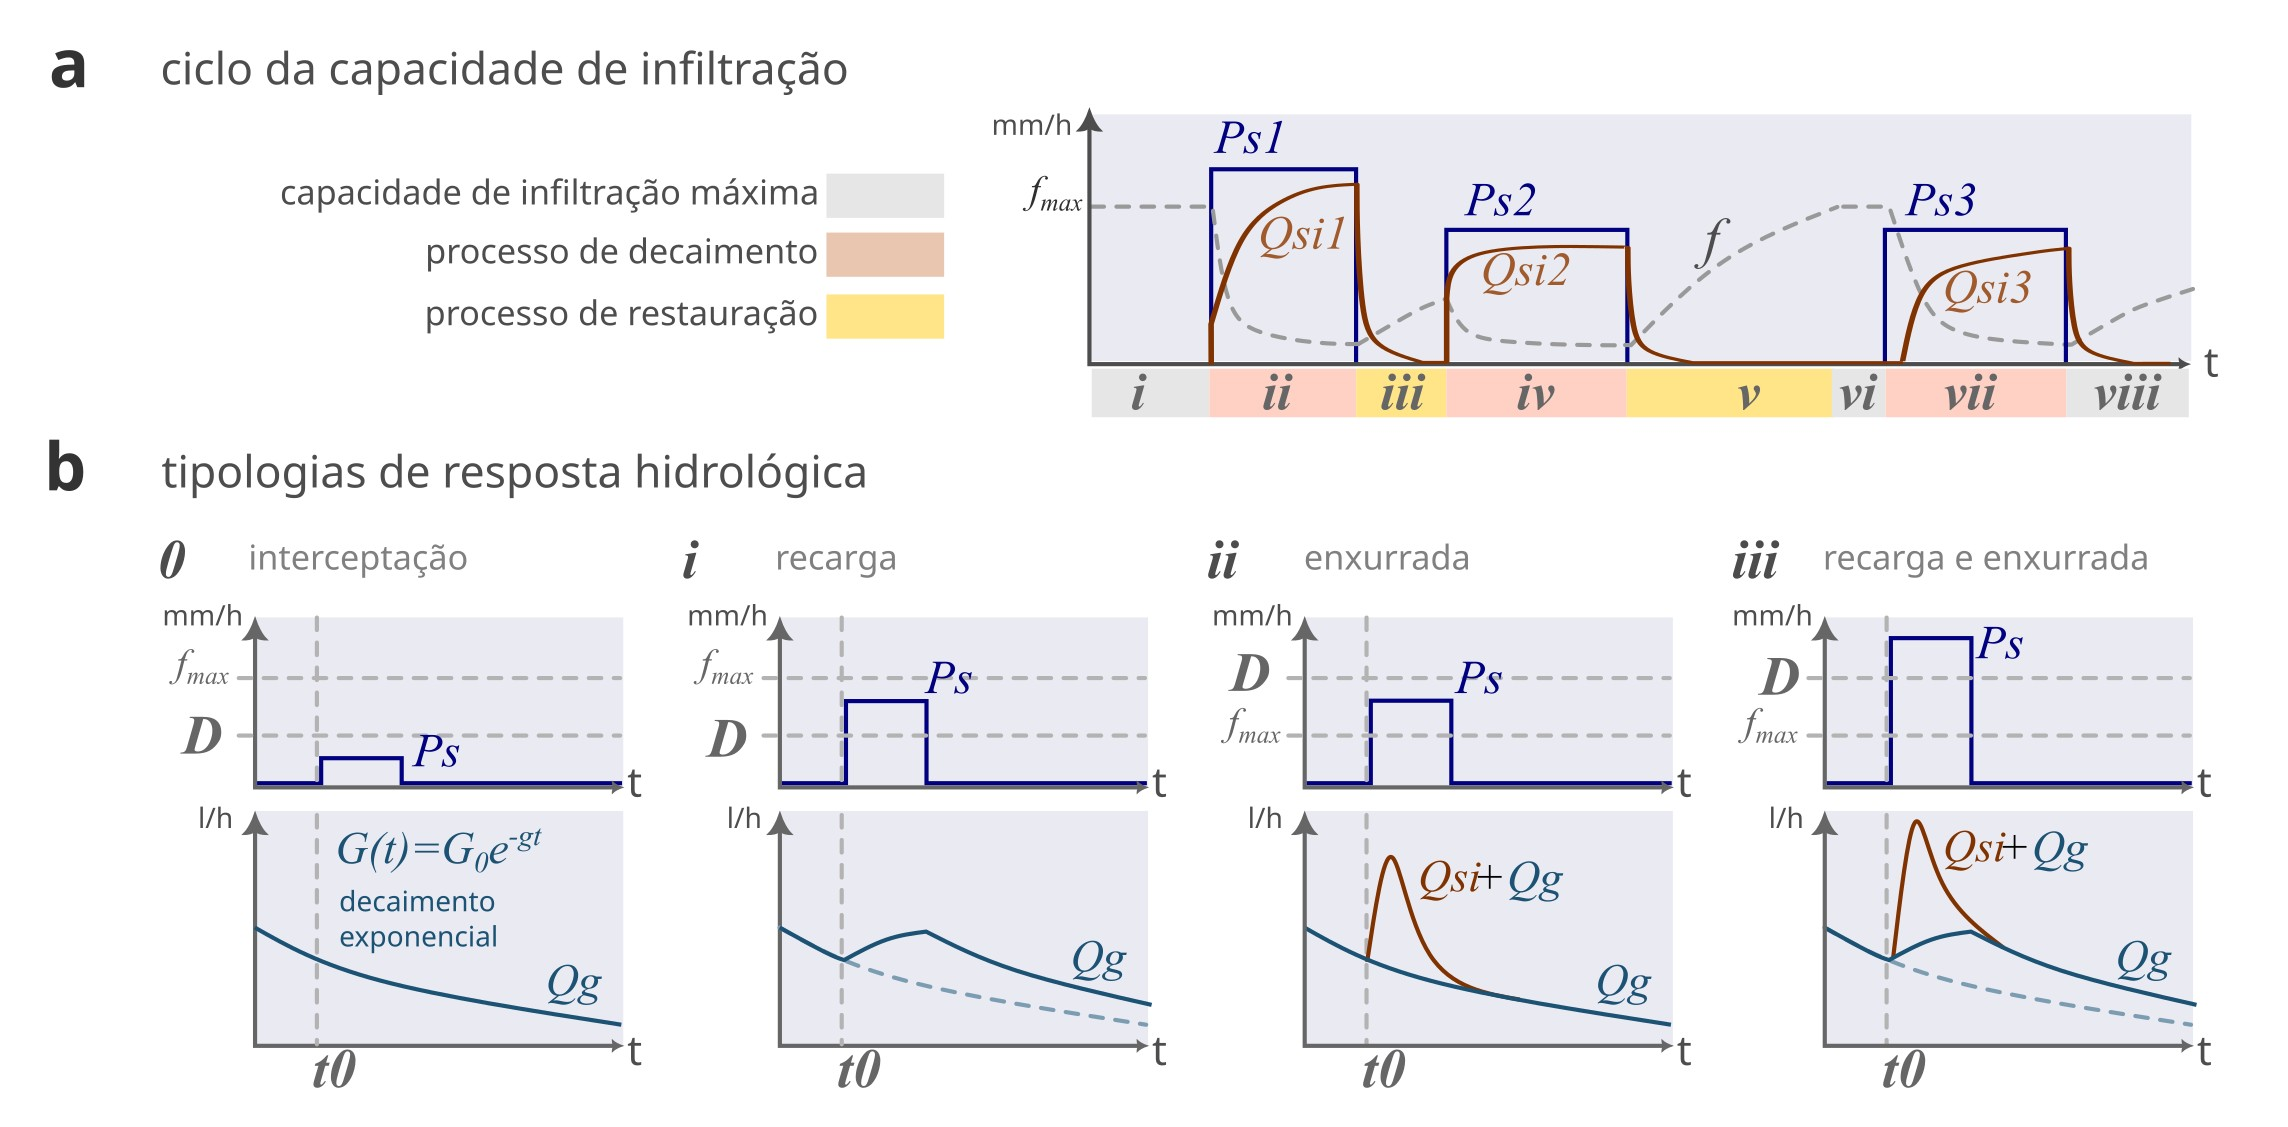
\includegraphics[width=0.98\linewidth]{figs/fig_horton2.jpg}		
\caption[Implicações do \gls{model} Hortoniano]
{\textbf{---\;Implicações do \gls{model} Hortoniano.}
    \textbf{a}\;---\;A capacidade de \gls{infiltration} passa por ciclos de decaimento e restauração, gerando não-linearidades, como o fato de chuvas idênticas ($P_{g,2}$ e $P_{g,3}$) produzirem respostas rápidas diferentes ($Q_{s,2}$ e $Q_{s,3}$) (detalhes \textrm{\textit{iv}} e \textrm{\textit{vii}}.\;\textbf{b}\;---\;É possível também deduzir diferentes tipologias de \gls{hydro-response}: Tipo 0, quando a chuva não produz recarga nem enxurrada (sem resposta, detalhe \textrm{\textit{0}}); Tipo 1, quando a chuva produz apenas recarga (resposta lenta, detalhe \textrm{\textit{i}}); Tipo 2, quando a chuva produz apenas enxurrada (resposta rápida, detalhe \textrm{\textit{ii}}), e; Tipo 3, quando a chuva produz tanto uma resposta lenta quanto rápida (detalhe \textrm{\textit{iii}}).
}
\label{fig:hydro:horton2} 		
\end{figure}

\par Diante desse \gls{percept-model}, diversos modelos conceituais foram então desenvolvidos por abordagens físicas (quando princípios físicos são aplicados \textit{a priori}) e empíricas (quando equações são ajustadas aos dados \textit{a posteriori})  \cite{mishra2003}. Na linha da abordagem física, destacam-se os avanços de Philip (1957) \cite{philip1957}, que arquitetou os fundamentos de uma \gls{teoria} matematicamente formal da infiltração como um caso especial da equação de Darcy-Richards, ou seja, do movimento da água em um meio poroso não saturado. Pelo lado empírico, o próprio Robert Horton manteve uma linha de pesquisa aplicada, propondo um \gls{concept-model} de decaimento exponencial para a \gls{infmax} do solo \cite{Horton1939}. Com isso, a produção de curvas de infiltração padronizadas experimentalmente viabilizou uma técnica mais sofisticada para se estimar o total de \gls{sf-runoff}, em contraste com o método racional, que é baseado em um simples coeficiente de escoamento \cite{Cook1946}. Outro método empírico de grande influência prática produzido nesse contexto foi o \textbf{\gls{cn_method}}, que foi desenvolvido pelo \acrfull{scs}\footnote{Atual \acrfull{usda}} em 1954 e apresentado como uma diretriz técnica nas décadas seguintes. De acordo com Rallison \& Miller (1981) \cite{Rallison1981}, o método \acrshort{cn} do \acrshort{scs} surgiu levando em conta os resultados de pesquisas experimentais em pequenas bacias, mas foi principalmente motivado pela aprovação de uma legislação de proteção ambiental nos Estados Unidos. Consta que Horton foi consultor do \acrshort{scs}, mas o seu método das curvas de infiltração não teve muito sucesso, cedendo lugar à abordagem agregada de Mockus (1949) \cite{mockus1949}, que avalia a relação entre os totais de chuva e escoamento para eventos individuais. Justificada por essas evidências, a equação do método \acrshort{cn}\footnote{A equação do método \acrshort{scs} é dada por: $R = \frac{(P - I_a)^{2}}{(P - I_a + S)}$, em que $R$ (mm) é a \gls{sf-runoff} total, equivalente à \gls{ex-rain}; $P$ é a chuva total (mm); $S$ (mm) é a \gls{sfmax}, calculada pelo parâmetro CN: $S = \frac{1000}{\text{CN}}-10$, e; $I_a$ (mm) são as abstrações iniciais (incluindo infiltração e interceptação), calculada ao se assumir que $I_a = 0.2S$. De acordo com Rallison \& Miller (1981) \cite{Rallison1981}, a equação emerge do balaço hídrico da \gls{ground-rain} e segundo a premissa de que a razão entre \gls{sf-runoff} e chuva efetiva ($P - I_a$) é a mesma que a razão entre a detenção superficial ($F$) e a capacidade de detenção ($S$), ou seja: $Q/(P-I_a) = F/S$. Talvez o método \acrshort{cn} pareça menos arbitrário se os dados de Mockus e Sherman forem interpretados como a marca de um \textit{processo de saturação} superficial, o que resulta em uma equação homóloga.} busca expressar a suposta \textit{transição} de uma resposta \textit{não-linear} (quando a infiltração e detenção superficial dominam o balanço de água superficial) para uma resposta \textit{linear} (quando a intensidade da \gls{ground-rain} é superior à \gls{infmax} e detenção superficial). O parâmetro CN, nesse sentido, calibra o efeito da não-linearidade para diferentes tipos de solo, coberturas, práticas de manejo e condições antecedentes de umidade. Rallison \& Miller apontam que a escolha dessa abordagem pelo \acrshort{scs} teve um forte viés de conveniência, pois os dados utilizados estavam prontamente disponíveis em escala nacional (nos Estados Unidos). Não obstante, a essência do método \acrshort{cn} reproduz o \gls{percept-model} de Horton, pois a \gls{sf-runoff} é tido como a única resposta rápida da bacia hidrográfica e é determinada pela estimativa da \gls{ex-rain}. 

\section{Diferenciação}

\begin{figure}[t!] 
\centering				
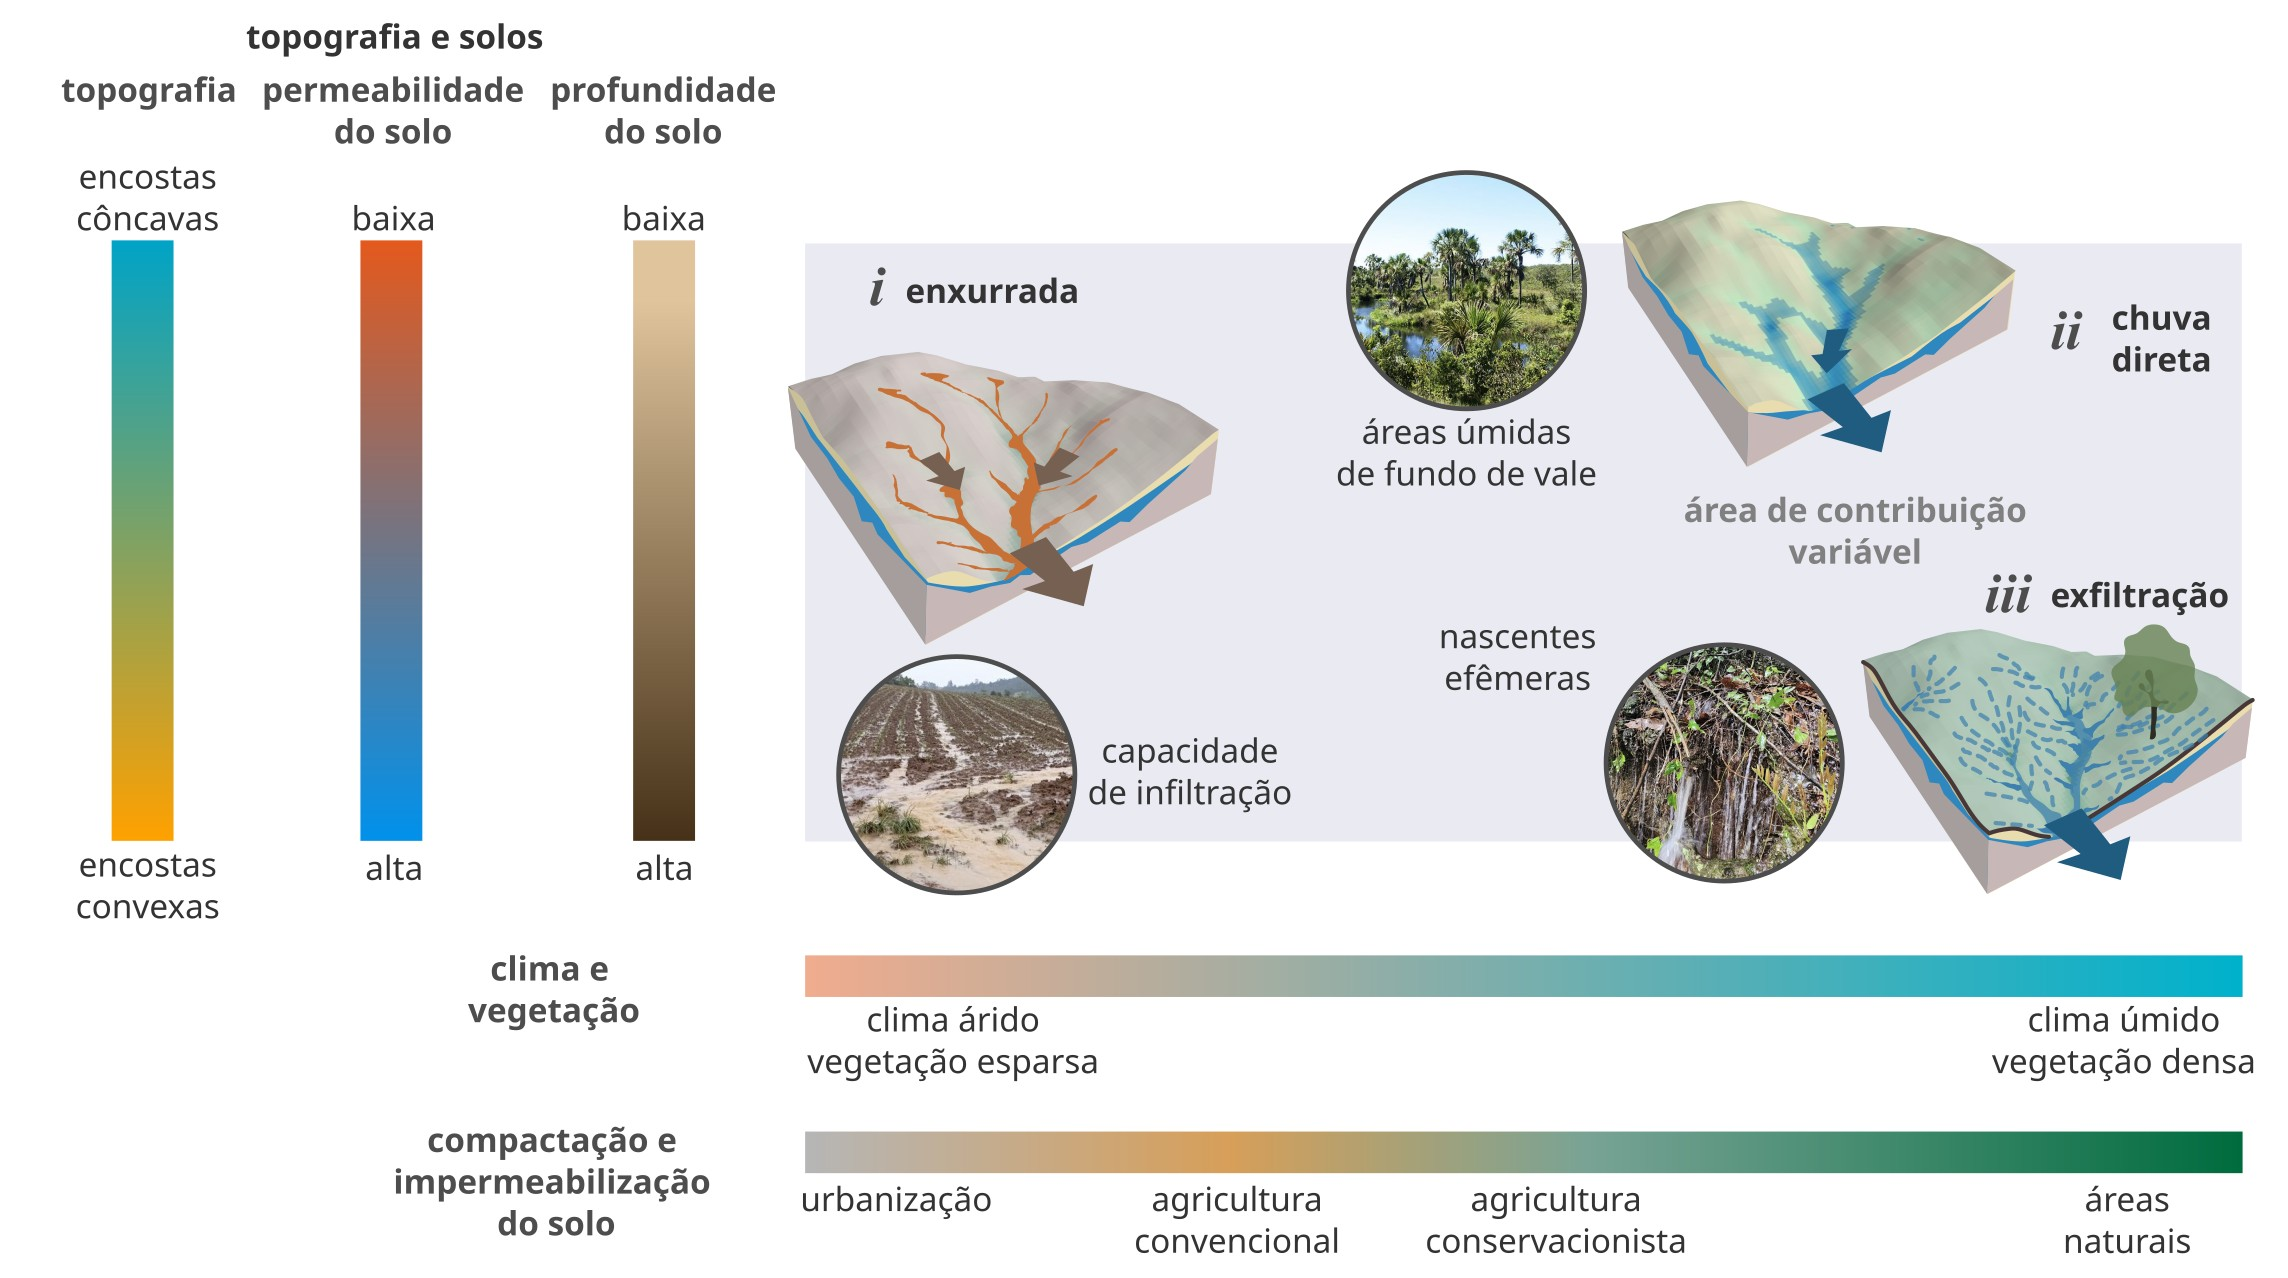
\includegraphics[width=0.98\linewidth]{figs/fig_processes.jpg}		
\caption[Diferenciação dos mecanismos de resposta rápida.]
{\textbf{---\;Diferenciação dos mecanismos de resposta rápida.}
    Visão esquemática proposta por Thomas Dunne (1983) \cite{Dunne1983} sobre o novo \gls{paradigma} dos mecanismos de respostas rápidas em bacias de ordem zero. As enxurradas, tidas como o único mecanismo no \gls{paradigma} Hortoniano, foram reservadas para condições especiais de climas áridos ou ambientes antropizados, como lavouras ou cidades, onde a capacidade de infiltração do solo é muito baixa (detalhe \textrm{\textit{i}}). Pelo menos dois novos mecanismos são diferenciados: respostas rápidas por excesso de saturação, ou chuva direta sobre \gls{sat_areas} (detalhe \textrm{\textit{ii}}), e; respostas rápidas por exfiltração em \gls{nasc_efemeras}, dominantes em solos mais profundos e estruturados com macroporos (detalhe \textrm{\textit{iii}}).
}
\label{fig:hydro:diff} 		
\end{figure}

\par Na Seção \ref{sec:epis:kuhn} ressaltei que, segundo Thomas Kuhn, o sucesso de uma \gls{teoria} científica está principalmente associado com a sua \textit{competitividade} em relação a outras ideias que circulam pela \gls{comunidade-cientifica}. Assim, uma \gls{teoria} tende a se estabelecer como o \gls{paradigma} hegemônico quando ela é eficiente tanto em explicar os fenômenos conhecidos quanto em abrir frentes de investigação promissoras para as novas gerações de pesquisadores. Na ausência de teorias concorrentes estruturadas nesse sentido, o \gls{percept-model} de Horton para explicar as respostas hidrológicas rápidas e lentas entregou esses dois atributos para uma \gls{comunidade-cientifica} fortemente marcada pelo \gls{bias-engineer} e pelo \gls{bias-fluvial}. Essas duas características possuem um efeito de blindar as percepções que tecnicamente são irrelevantes para solucionar os típicos problemas de jusante, pois não precisam dos detalhes sobre o que acontece nas bacias de ordem zero\footnote{Ironicamente, era exatamente esse o objetivo do \acrshort{scs} -- proteger o solo nas encostas.}. O \gls{model} Hortoniano, mesmo que parcial ou completamente incorreto, não impediu que fossem feitas boas estimativas de vazões de projeto para pontes, barragens, balanço hídrico em grandes bacias, etc. Afinal, a equifinalidade dos sistemas permite que comportamentos semelhantes se manifestem a partir de mecânicas distintas (até o dia que todos são surpreendidos). No âmbito estritamente técnico, em certa medida, o desenvolvimento do método \acrshort{cn} pelo \acrshort{scs} \textit{perpetuou} as ideias da \gls{age_inf}, sendo geralmente o método básico exigido ou aceito por diretrizes técnicas em projetos de engenharia e o principal módulo de geração de escoamento em diversos modelos hidrológicos distribuídos em \textit{softwares}, como o \texttt{SWAT} e \texttt{SWMM}\footnote{Na minha graduação como Engenheiro Ambiental fui treinado a aplicar o método racional e \acrshort{cn} para estimativa de \say{vazões de projeto}. Inclusive, durante meu intercâmbio nos Estados Unidos em 2014-2015, ganhei uma cópia impressa da \textit{Technical Release} 55 do \acrshort{usda}, que basicamente é a versão mais recente do método \acrshort{cn} aplicada em projetos de drenagem urbana nos Estados Unidos.}. 

\par Apesar de que talvez o \gls{paradigma} da infiltração tenha se consolidado simplesmente pela falta de competidores, a sua crise esteve presente desde a sua formação, nos anos 1930 e 1940. Por exemplo, os dados de intensidade de chuva e \gls{infmax} do solo medidos pelo próprio laboratório de Robert Horton sugerem que é muito \textit{improvável} que ele mesmo tenha observado \gls{sf-runoff} generalizada na sua bacia experimental em La Grange Brook (14.4 ha, Nova Iorque) \cite{Beven2004c}. Os dados do laboratório, avaliados por Keith Beven, indicam que o solo nas principais coberturas da bacia (campos e pomares) apresentava uma \gls{infmax} relativamente alta diante das chuvas registradas. Na verdade, a conciliação entre as medições feitas por Horton da \gls{infmax} do solo \textit{in situ}, o \textbf{valor de campo}, com estimativas na escala de bacia, o \textbf{valor efetivo}, possivelmente nunca fizeram muito sentido entre si, exigindo numerosas \gls{aux-hyp} e \gls{neglig-premis} (o \textbf{problema da escala}, que veremos adiante). Isso ficou claro no artigo de Betson (1964) \cite{Betson1964}, que conseguiu excelentes ajustes de um \gls{concept-model} aos dados observados somente após \textit{relaxar} o \gls{model} Hortoniano, implicando um conceito \textbf{área de contribuição parcial} de escoamento superficial\footnote{Do ponto de vista racionalista, Betson tentou \say{salvar} a \gls{teoria} de Horton, admitindo modificações \textit{ad hoc} para evitar a sua refutação.}. Ainda que estatisticamente bem ajustados, os resultados insinuavam que uma fração pequena e relativamente constante nas bacias no vale do Rio Tennessee produziam \gls{sf-runoff} (bacias entre 500 ha até 8,4 km², Carolina do Norte).

\par Mas foi ao longo da década de 1960 que a \gls{age_inf} encontrou sua crise derradeira no âmbito científico. Não por acaso, esse período testemunhou a \textbf{Década Hidrológica Internacional} (1965-1974), um programa das Nações Unidas (\texttt{UNESCO}) desenvolvido com o objetivo de promover a pesquisa na \gls{hydrology}. A revolução nas percepções da \gls{comunidade-cientifica} ocorreu após uma profusão de evidências empíricas acumularem-se na literatura, relatando a observação de novos mecanismos de \gls{hydro-response} das encostas, que serão descritas nas próximas seções. Pode-se resumir o advento de pelo menos três novos mecanismos de resposta rápida (ou potencialmente rápida) além daquele postulado por Horton: (1) \textbf{\gls{subsur_flow}}\footnote{Esse mecanismo, além do estranho nome de \say{afloramento pluvial} (\textit{storm-seepage}), também foi denominado na literatura por diversos outros títulos: fluxo de retorno (\textit{return flow}), fluxo de passagem (\textit{throughflow}), interfluxo (\textit{interflow}), fluxo lateral (\textit{lateral flow}) e escoamento subsuperficial (\textit{exfiltration}).}; (2) \textbf{\gls{rse}}\footnote{Tradução livre de: \textit{saturation-excess runoff}.}, e; (3) \textbf{\gls{trans_flow}}\footnote{Tradução livre de: \textit{translational flow}.}. Os dois primeiros se referem à água nova da chuva que contribui para as enchentes. O último consiste na água velha armazenada no subsolo, que também contribui para a resposta rápida (com taxas de prevalências surpreendentes). A nomenclatura sobre esses mecanismos é um tanto confusa na literatura ainda hoje, talvez em consequência do fato da água não ter um rótulo visível, o que dificulta a diferenciação fora de contexto (por exemplo, o afloramento da água em nascentes pode ser tanto uma resposta lenta quanto rápida). Em contraste com o \gls{model} Hortoniano, essas respostas rápidas incluem rotas superficiais e subterrâneas controladas por outras partes do \gls{system} além da camada superficial do solo, como a \textbf{\gls{macropor}} (caminhos preferenciais laterais e verticais no solo) e a topografia (padrões dinâmicos de saturação do solo). Em essência, as evidências empíricas na segunda metade do século XX expuseram irreversivelmente a complexidade dos processos em bacias de ordem zero. 

\par Um marco para o início do fim da \gls{age_inf} foi o artigo de Mike Kirkby (1969) \cite{Kirkby1969}, que revisou resultados de diversos estudos experimentais e apresentou didaticamente uma nova forma de compreender e nomear os processos hidrológicos em bacias de ordem zero. Nesse ponto, Kirkby (1969) demarca definitivamente a importância das respostas rápidas de água que transita no solo por uma rede de macroporos (escoamento subsuperficial). Após mais de uma década de novas evidências empíricas se acumulando, um marco para a ascensão do novo \gls{paradigma} foi o artigo de Thomas Dunne (1983) \cite{Dunne1983}, que organizou definitivamente uma nova visão esquemática sobre as respostas hidrológicas rápidas, ilustrada na Figura \ref{fig:hydro:diff}, propondo um novo programa promissor de pesquisas nas frentes pura e aplicada. Dunne (1983) deixa claro a ideia de que diferentes climas, escalas e paisagens favorecem a \textit{dominância} de um ou de outro mecanismo, ainda que eles possam acontecer simultaneamente ou se alternar sazonalmente. Por exemplo, em climas semi-áridos, fatores como os longos períodos de estiagem e a formação de crostas no solo favorecem o mecanismo de Horton -- a \gls{infmax} tende a ser insuficiente e sequer existem áreas saturadas nos fundos de vale no final da estação seca. Em climas tropicais úmidos, por outro lado, a formação de solos profundos ou o excesso de água na estação chuvosa pode favorecer tanto um mecanismo quanto outro. Por fim, essa revolução produziu novos entendimentos sobre a complexa relação desses mecanismos, como demonstrado por Jeffrey McDonnell (1990) \cite{mcdonnell1990} no caso da Bacia Experimental de MaiMai (Nova Zelândia). Mas McDonnell (2013) \cite{Mcdonnell2013} também estabelece uma crítica ao \gls{paradigma} que se instalou: o programa de pesquisa hegemônico se pauta principalmente em \textit{diferenciar} as múltiplas respostas hidrológicas, reafirmando a ideia de complexidade e singularidade de cada ambiente. Ainda que essa atitude possa seguir \textit{ad infinitum}, ele argumenta que o objetivo verdadeiro de uma ciência hidrológica talvez seja o de produzir \textit{generalizações}, teorias que sejam \textit{unificadoras}. Nesse espírito, o \gls{paradigma} hidrológico vigente talvez mereça o título de \textbf{\gls{age_diff}}.

\subsection{Macroporos}

% figure
\begin{figure}[t!] 
\centering				
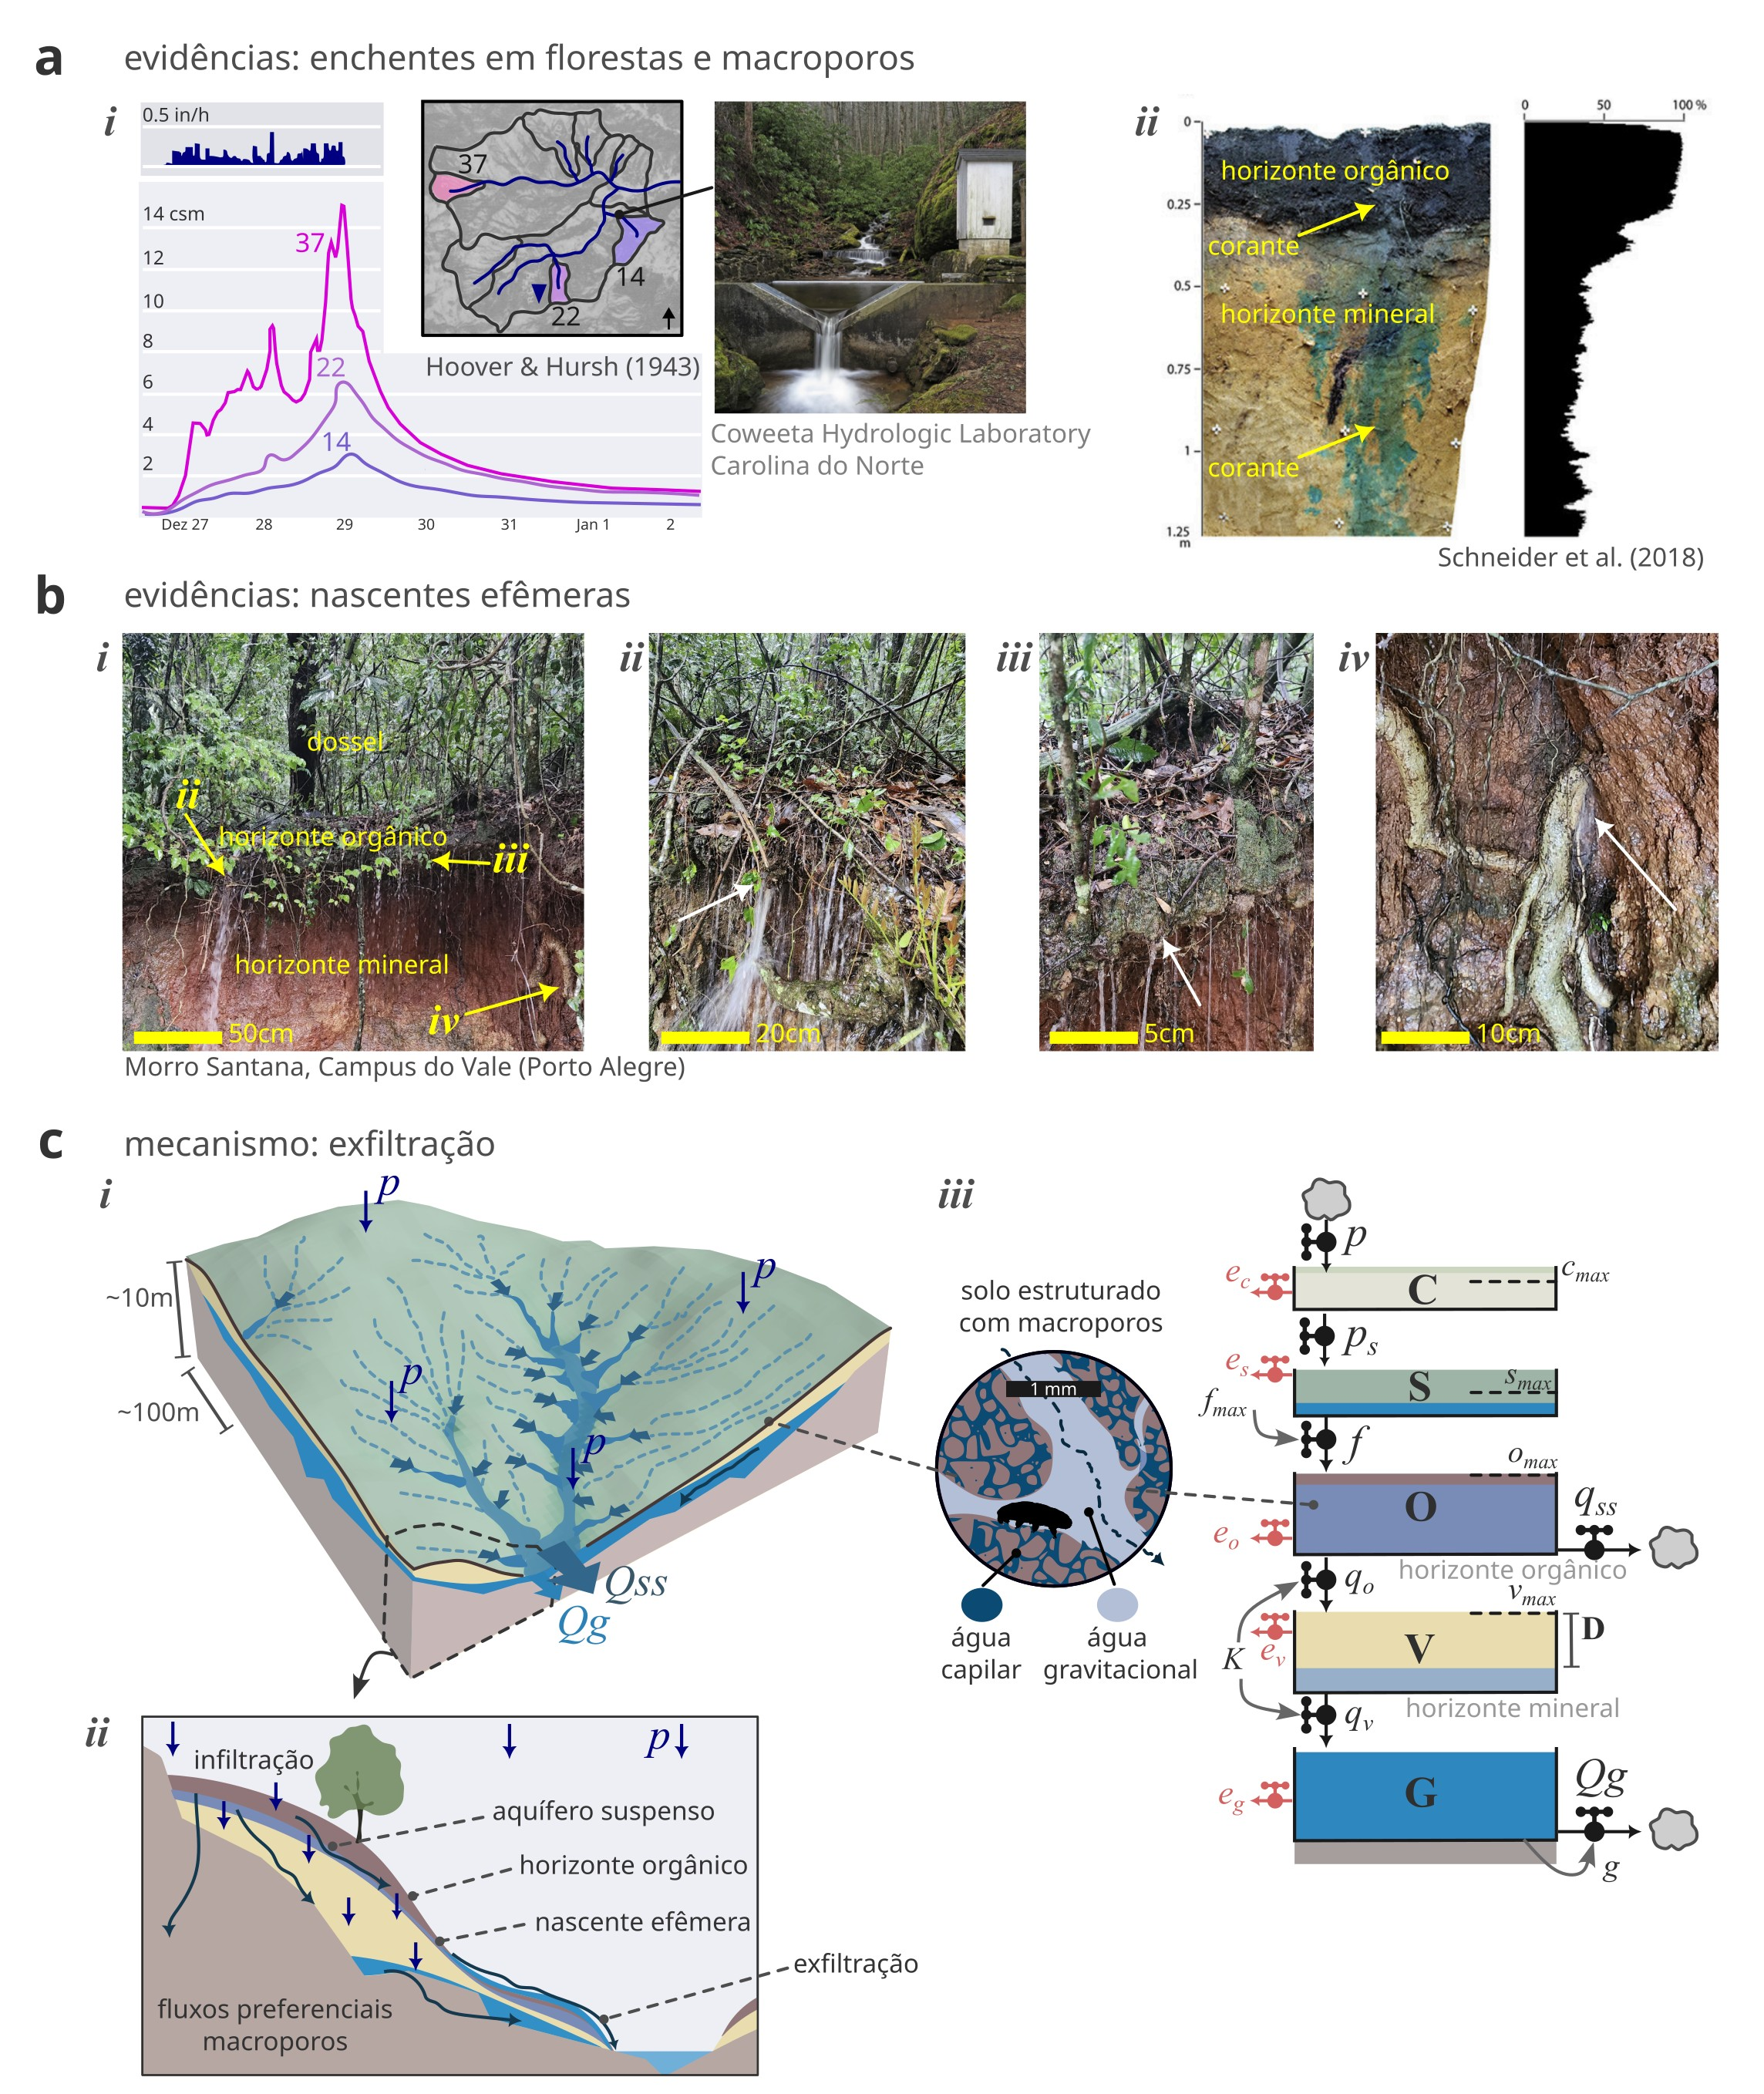
\includegraphics[width=0.98\linewidth]{figs/fig_macropores.jpg}		
\caption[Exfiltração rápida por macroporos]
{\textbf{---\;Exfiltração rápida por macroporos.}
    Macroporos e caminhos preferenciais subterrâneos produzem respostas rápidas de \gls{subsur_flow}, especialmente em florestas.\;\textbf{a}\;---\;Evidências: enchentes sem enxurradas em bacias na Floresta Experimental de Coweeta (Carolina do Norte, Estados Unidos) reportadas por Hoover \& Hursh (1943) \cite{Hoover1943} (detalhe \textrm{\textit{i}}), e; a distribuição de macroporos no perfil do solo realçadas por corantes, reportada por Schneider et \textit{al.} (2018) \cite{Schneider2018} (detalhe \textrm{\textit{i}}).\;\textbf{b}\;---\;Evidências: \gls{nasc_efemeras} observadas em 16 de Junho de 2023 em um corte de estrada no Campus do Vale da Universidade Federal do Rio Grande do Sul (Morro Santana, Porto Alegre). Apesar da chuva extraordinária nesse dia (141,7 mm em 24 horas), não se observou enxurradas no solo da floresta. \textrm{\textit{i}} -- perfil do barranco; \textrm{\textit{ii}} -- fluxo preferencial; \textrm{\textit{iii}} escoamento na interface entre horizontes; \textrm{\textit{iv}} -- escoamento turbulento em uma fratura no granito, criada por uma raiz.\;\textbf{c}\;---\;Sistematização do mecanismos de \gls{nasc_efemeras}: a água da chuva se infiltra rapidamente, criando um aquífero suspenso na transição entre o horizonte orgânico e mineral. Esse aquífero suspenso aflora em diversos pontos da bacia, facilitado por macroporos e caminhos preferenciais subterrâneos, criando \gls{nasc_efemeras} durante e logo após a passagem da chuva. Fonte da fotografia em \textbf{a}: https://www.be-roberts.com/se/cwta/cwta1.htm .
}
\label{fig:hydro:macro} 		
\end{figure}

\par No final dos anos 1930 e início dos anos 1940, a literatura científica já reconhecia as fragilidades do \gls{model} de Horton, sustentando que a resposta rápida de pequenas bacias deveria incluir um ou mais mecanismos \textit{subterrâneos}. Snyder (1939) \cite{Snyder1939}, por exemplo, sugere o uso do termo escoamento direto\footnote{Tradução livre de \textit{direct-runoff}.} para denotar a água da chuva que contribui para a enchente do rio \textit{sem nunca ter transitado pelo solo}. Nesse contexto, Barnes (1939) \cite{Barnes1939} divide em \textit{três} (e não \textit{duas}) as componentes do escoamento fluvial\footnote{Tradução livre de \textit{stream-flow}.}: (1) escoamento superficial\footnote{Tradução livre de \textit{surface-flow}.}; (2) afloramento pluvial\footnote{Tradução livre de \textit{storm-seepage}.} e; (3) escoamento de base\footnote{Tradução livre de \textit{base-flow}.}. Por \say{afloramento pluvial} (\textit{storm-seepage}) Barnes se referia a um escoamento subterrâneo rápido da água da chuva que se move \textit{lateralmente} pela \gls{unsat-zone}, alimentando os canais dos riachos com uma velocidade muito superior ao que é esperado do \gls{g-coef}:

\begin{adjustwidth}{100pt}{0pt}
\medskip
\small Isto consiste na água que penetrou apenas nas camadas superiores do solo durante uma chuva ou degelo e filtrou-se mais ou menos horizontalmente através do solo para desaguar no \gls{system} de rios por afloramentos. Esse fenômeno foi observado pelo autor em 1936 enquanto analisava os dados de vazão do Rio Zumbro em Minnesota e denominado por ele como \say{fluxo de base secundário}.\footnote{Tradução livre de: \textit{This consists of water which has penetrated only the upper soil-layers during a rainstorm or a thaw and has filtered more or less horizontally through the soil to discharge into the stream-system by seepage. It was observed by the writer in 1936 while analyzing discharge records of Zumbro River in Minnesota and called by him \say{secondary base-flow}.}} -- Bertram Barnes (1939, p. 721) \cite{Barnes1939}.
\medskip
\end{adjustwidth}

\noindent Assim, é feita uma diferença entre as \textbf{\gls{nasc_perenes}}, alimentadas pelo escoamento da água subterrânea \say{verdadeira} (aquífero livre), das \textbf{\gls{nasc_efemeras}}, alimentadas pela \gls{subsur_flow} da água da chuva (aquífero suspenso). Esse mecanismos de resposta foi imensamente reforçado por estudos conduzidos por Charles Hursh na Floresta Experimental de Coweeta (Carolina do Norte, Estados Unidos), com resultados reportados para diversas bacias florestadas com áreas entre 16 a 760 hectares \cite{Hoover1943, Hursh1944}, gerando o \gls{model} ilustrado nos detalhes da Figura \ref{fig:hydro:macro}\textbf{c}. Por exemplo, Hursh \& Brater (1941) \cite{Hursh1941} alegam que jamais se observou \gls{sf-runoff} nas encostas de uma das bacias monitoradas, apesar das respostas rápidas observadas na vazão do rio: 

\begin{adjustwidth}{100pt}{0pt}
\medskip
\small O escoamento das chuvas na forma de \gls{sf-runoff} não foi observado nesta área de drenagem; ainda assim, hidrogramas de enchentes característicos são produzidos por chuvas intensas.\footnote{Tradução livre de: \textit{Surface storm-runoff as overland-flow has not been observed on this drainage-area; nevertheless, characterlstlc flood-hydrographs are produced by heavy rains.}} -- Hursh \& Brater (1941, p. 863) \cite{Hursh1941}.
\medskip
\end{adjustwidth}

\noindent Essa alegação, seguida de dados em estudos subsequentes (ver Figura \ref{fig:hydro:macro}\textbf{a}, no detalhe \textit{i}) fatalmente introduz um \textit{contra-exemplo} para a \gls{teoria} da \gls{infmax}.  Afinal, se não há \gls{sf-runoff}, a única resposta disponível no \gls{percept-model} de Horton é a resposta \textit{lenta} causada pela \gls{qv} do aquífero, responsável pela \gls{deple-curve}. Entre outros mecanismos em ação na bacia, detalhados mais adiante, os autores apontam a existência de respostas \textit{subterrâneas rápidas} que incluem tanto o fluxo de água em camadas de solo altamente permeáveis (fluxo não saturado), quanto a formação de aquíferos suspensos temporários (fluxo saturado), que se desenvolvem em diferentes partes da paisagem durante as chuvas. Nessa direção, Hursh \& Fletcher (1942) \cite{Hursh1942} salientam a importância da \gls{macropor} do solo. Especialmente em florestas, essa propriedade ajudaria a explicar a dominância de fluxos preferenciais subsuperficiais, aumentando tremendamente a \gls{water_gravit} do solo, em oposição à \gls{water_capilar}:

\begin{adjustwidth}{100pt}{0pt}
\medskip
\small A natureza exata deste espaço macroporoso ocorrendo em diferentes horizontes do perfil do solo ainda precisa ser descrita. Ela inclui todos os grandes canais subterrâneos formados por raízes decompostas, rochas fraturadas, túneis de insetos e animais, e espaços maiores que possam existir. Também inclui espaços macroporosos formados através dos complexos padrões estruturais criados pela agregação de partículas do solo na presença de materiais orgânicos. Nos horizontes superiores dos solos naturais, essas aberturas biológicas e padrões estruturais construídos a partir de agregados semelhantes a treliças são muito mais importantes na determinação da porosidade não capilar do que o tamanho das partículas individuais do solo. Canais de raízes e túneis de animais são particularmente significativos no armazenamento e drenagem da \gls{water_gravit}. Um único túnel de minhoca pode ser muito mais importante na drenagem de um bloco de solo maciço do que toda a área da seção transversal do espaço poroso. Da mesma forma, é concebível que alguns poucos espaços vazios contínuos possam dar origem a uma descarga rápida de água subterrânea através de um perfil de solo que, quando visto como um meio uniformemente permeável, seria esperado transmitir água lentamente.\footnote{Tradução livre de: \textit{The exact nature of this macro-pore space occurring in different horizons of the soil profile has yet to be described. It includes all large underground channels formed from decayed roots, fractured rock, insect and animal burrows, and larger spaces that may exist. It also includes macro-pore spaces formed through the complex structural patterns created by the aggregation of soil particles in the presence of organic materials. In the upper horizons of natural soils these biological openings and structural patterns built up from lattice-like aggregates are far more important in determining noncapillary porosity than the single grain soil particle size. Root channels and animal burrows are of particular significance in the detention storage and draining of gravitational water. A single earthworm burrow may be far more important in draining through a block of heavy soil than the entire cross sectional area of the pore space. In like manner, it is conceivable that a few continuous void spaces may give rise to rapid discharge of groundwater through a soil profile which, when viewed as a uniformly pervious medium, would be expected to transmit water slowly.}} -- Hursh \& Fletcher (1942, p. 485) \cite{Hursh1942}.
\medskip
\end{adjustwidth}

\par Ao contrário de estudos recentes com corantes, que demonstram claramente a existência dos macroporos (como no detalhe \textit{ii} da Figura \ref{fig:hydro:macro}\textbf{a}, com os resultados recentes de Schneider et \textit{al.} (2018) \cite{Schneider2018}) os autores de Coweeta não apresentaram evidências além de observações de processos agregados, como chuva, vazão e níveis de poços. Essa lacuna de pesquisa foi permanentemente solucionada nos anos 1960, quando uma nova onda de estudos trouxe resultados quantitativos mais detalhados, obtidos por uma abordagem mais experimental do que observacional. Ainda no contexto da Floresta Experimental de Coweeta, Hewlett e Hibbert (1963) \cite{Hewlett1963} usaram um lisímetro para demonstrar o papel crítico do fluxo de água na \gls{unsat-zone} em sustentar o escoamento de base dos riachos. Whipkey (1965) \cite{Whipkey1965} detalhou os fluxos laterais no perfil de solo de uma encosta em Ohio (EUA). A encosta foi monitorada por uma trincheira na sua base, demonstrando a dinâmica do \gls{subsur_flow}, especialmente nas camadas orgânicas superiores, onde se mediu alta \gls{cond-hyd} devido aos macroporos. Aqui, aparece a função exercida pelas \textbf{\gls{perm_trans}} entre os horizontes do solo, especialmente entre o \gls{o-horizon} (superior) e o horizonte mineral (inferior). Essa descontinuidade gera uma perda de carga hidráulica que acaba causando um fluxo \textit{lateral} na \gls{unsat-zone}. Eu mesmo observei esse processo durante uma severa tempestade em 16 de Junho de 2023, no Campus do Vale da Universidade Federal do Rio Grande do Sul, na base do Morro Santana, Porto Alegre (ver detalhes na Figura \ref{fig:hydro:macro}\textbf{b})\footnote{Eu estava simplesmente indo almoçar no Restaurante Universitário do Campus, sem nenhuma intenção de registrar o evento. Ao passar de carro pelo acesso do restaurante, em meio à chuva, visualizei cascatas de água jorrando no barranco da estrada, o que me fez parar para investigar.}. Segundo a Estação \texttt{83967} do \texttt{INMET}, o dia 16 de Junho de 2023 acumulou 141,7 mm de chuva, o que é superior ao acumulado do mês pela normal climatológica desse mês (em torno de 130 mm). Mesmo diante de chuva tão extrema e dos riachos estarem praticamente transbordando, não observei enxurrada superficial nas florestas do Campus, a não ser onde o talvegue do terreno forçava o afloramento do aquífero suspenso (ou seja, pela expansão das áreas úmidas ripárias).

\par Outros estudos detalhados em trincheiras que chegaram em conclusões semelhantes aos de Whipkey (1965) nos Estados Unidos incluem: Ragan (1968), em Vermont \cite{Ragan1968}; Beasley (1976), no Mississippi \cite{Beasley1976}, e; Harr (1977), no Oregon \cite{Harr1977}. No último caso, relatou-se que o \gls{subsur_flow} foi de 6 a 9 vezes maior nas camadas superiores do solo que nas camadas inferiores, corroborando a função da \gls{macropor}. Nesse mesmo estudo, os autores relatam que a \gls{subsur_flow} foi responsável por cerca de 97\% da resposta rápida nas enchentes. Isso foi consistente com os resultados anteriores de Patric e Swanston (1968) \cite{patric1968}, que cortaram todas as árvores de uma encosta no Alasca e aplicaram irrigação por aspersão. Eles não observaram \gls{sf-runoff} -- a água aplicada percorreu caminhos subterrâneos preferenciais, aflorando rapidamente na base da encosta. Nas Ilhas Britânicas, Weyman (1970) \cite{weyman1970} reportou que o escoamento não-saturado subterrâneo consiste na principal resposta rápida em uma bacia experimental, enquanto que Jones (1971) \cite{Jones1971} fez observações de que a ocorrência generalizada do fenômeno de \textit{piping} -- a formação de túneis naturais no perfil do solo -- contribui para altas velocidades na resposta subterrânea. Consolidando essa nova geração de pesquisas de campo, os resultados a partir na bacia experimental MaiMai (Nova Zelândia) estabeleceram o novo programa de pesquisa experimental, com a aplicação combinada de balanço hídrico, trincheiras e a novidade dos traçadores químicos, corantes e isotópicos. No caso de MaiMai, Mosley (1979) \cite{Mosley1979} reafirma (quase quarenta anos depois de Hursh) o papel crucial da \gls{macropor} e túneis naturais na \gls{subsur_flow} ao rebater algumas objeções teóricas:

\begin{adjustwidth}{100pt}{0pt}
\medskip
\small Freeze [1972, p. 1282] considerou que um valor limiar de condutividade hidráulica saturada da ordem de 0,002 cm/s é necessário para que a \gls{subsur_flow} seja significativa, mas em um solo que contém canais de raízes, túneis e zonas de afloramento, a condutividade hidráulica saturada não é um fator limitante. O fluxo de corante traçador através de macroporos no solo foi observado a taxas até 3 ordens de magnitude maiores, e a resposta sensível e rápida da \gls{subsur_flow} às variações na precipitação sugere que o fluxo por macroporos, e não pela matriz do solo, contribui para as enchentes nos canais.\footnote{Tradução livre de: \textit{Freeze [1972, p. 1282] considered that a threshold value for saturated hydraulic conductivity of the order of 0,002 cm/s is necessary for subsurface stormflow to be significant, but in a soil that contains root channels, pipes, and seepage zones, saturated hydraulic conductivity is not a limiting factor. Flow of dye tracer through macropores in the soil was observed at rates up to 3 orders of magnitude greater, and the sensitive as rapid response of subsurface flow to variations in precipitation suggests that flow through macropores rather than through soil matrix contributes to channel stormflow.}} -- Paul Mosley (1979, p. 806) \cite{Mosley1979}.
\medskip
\end{adjustwidth}

\subsection{Topografia}

% figure
\begin{figure}[t!] 
\centering				
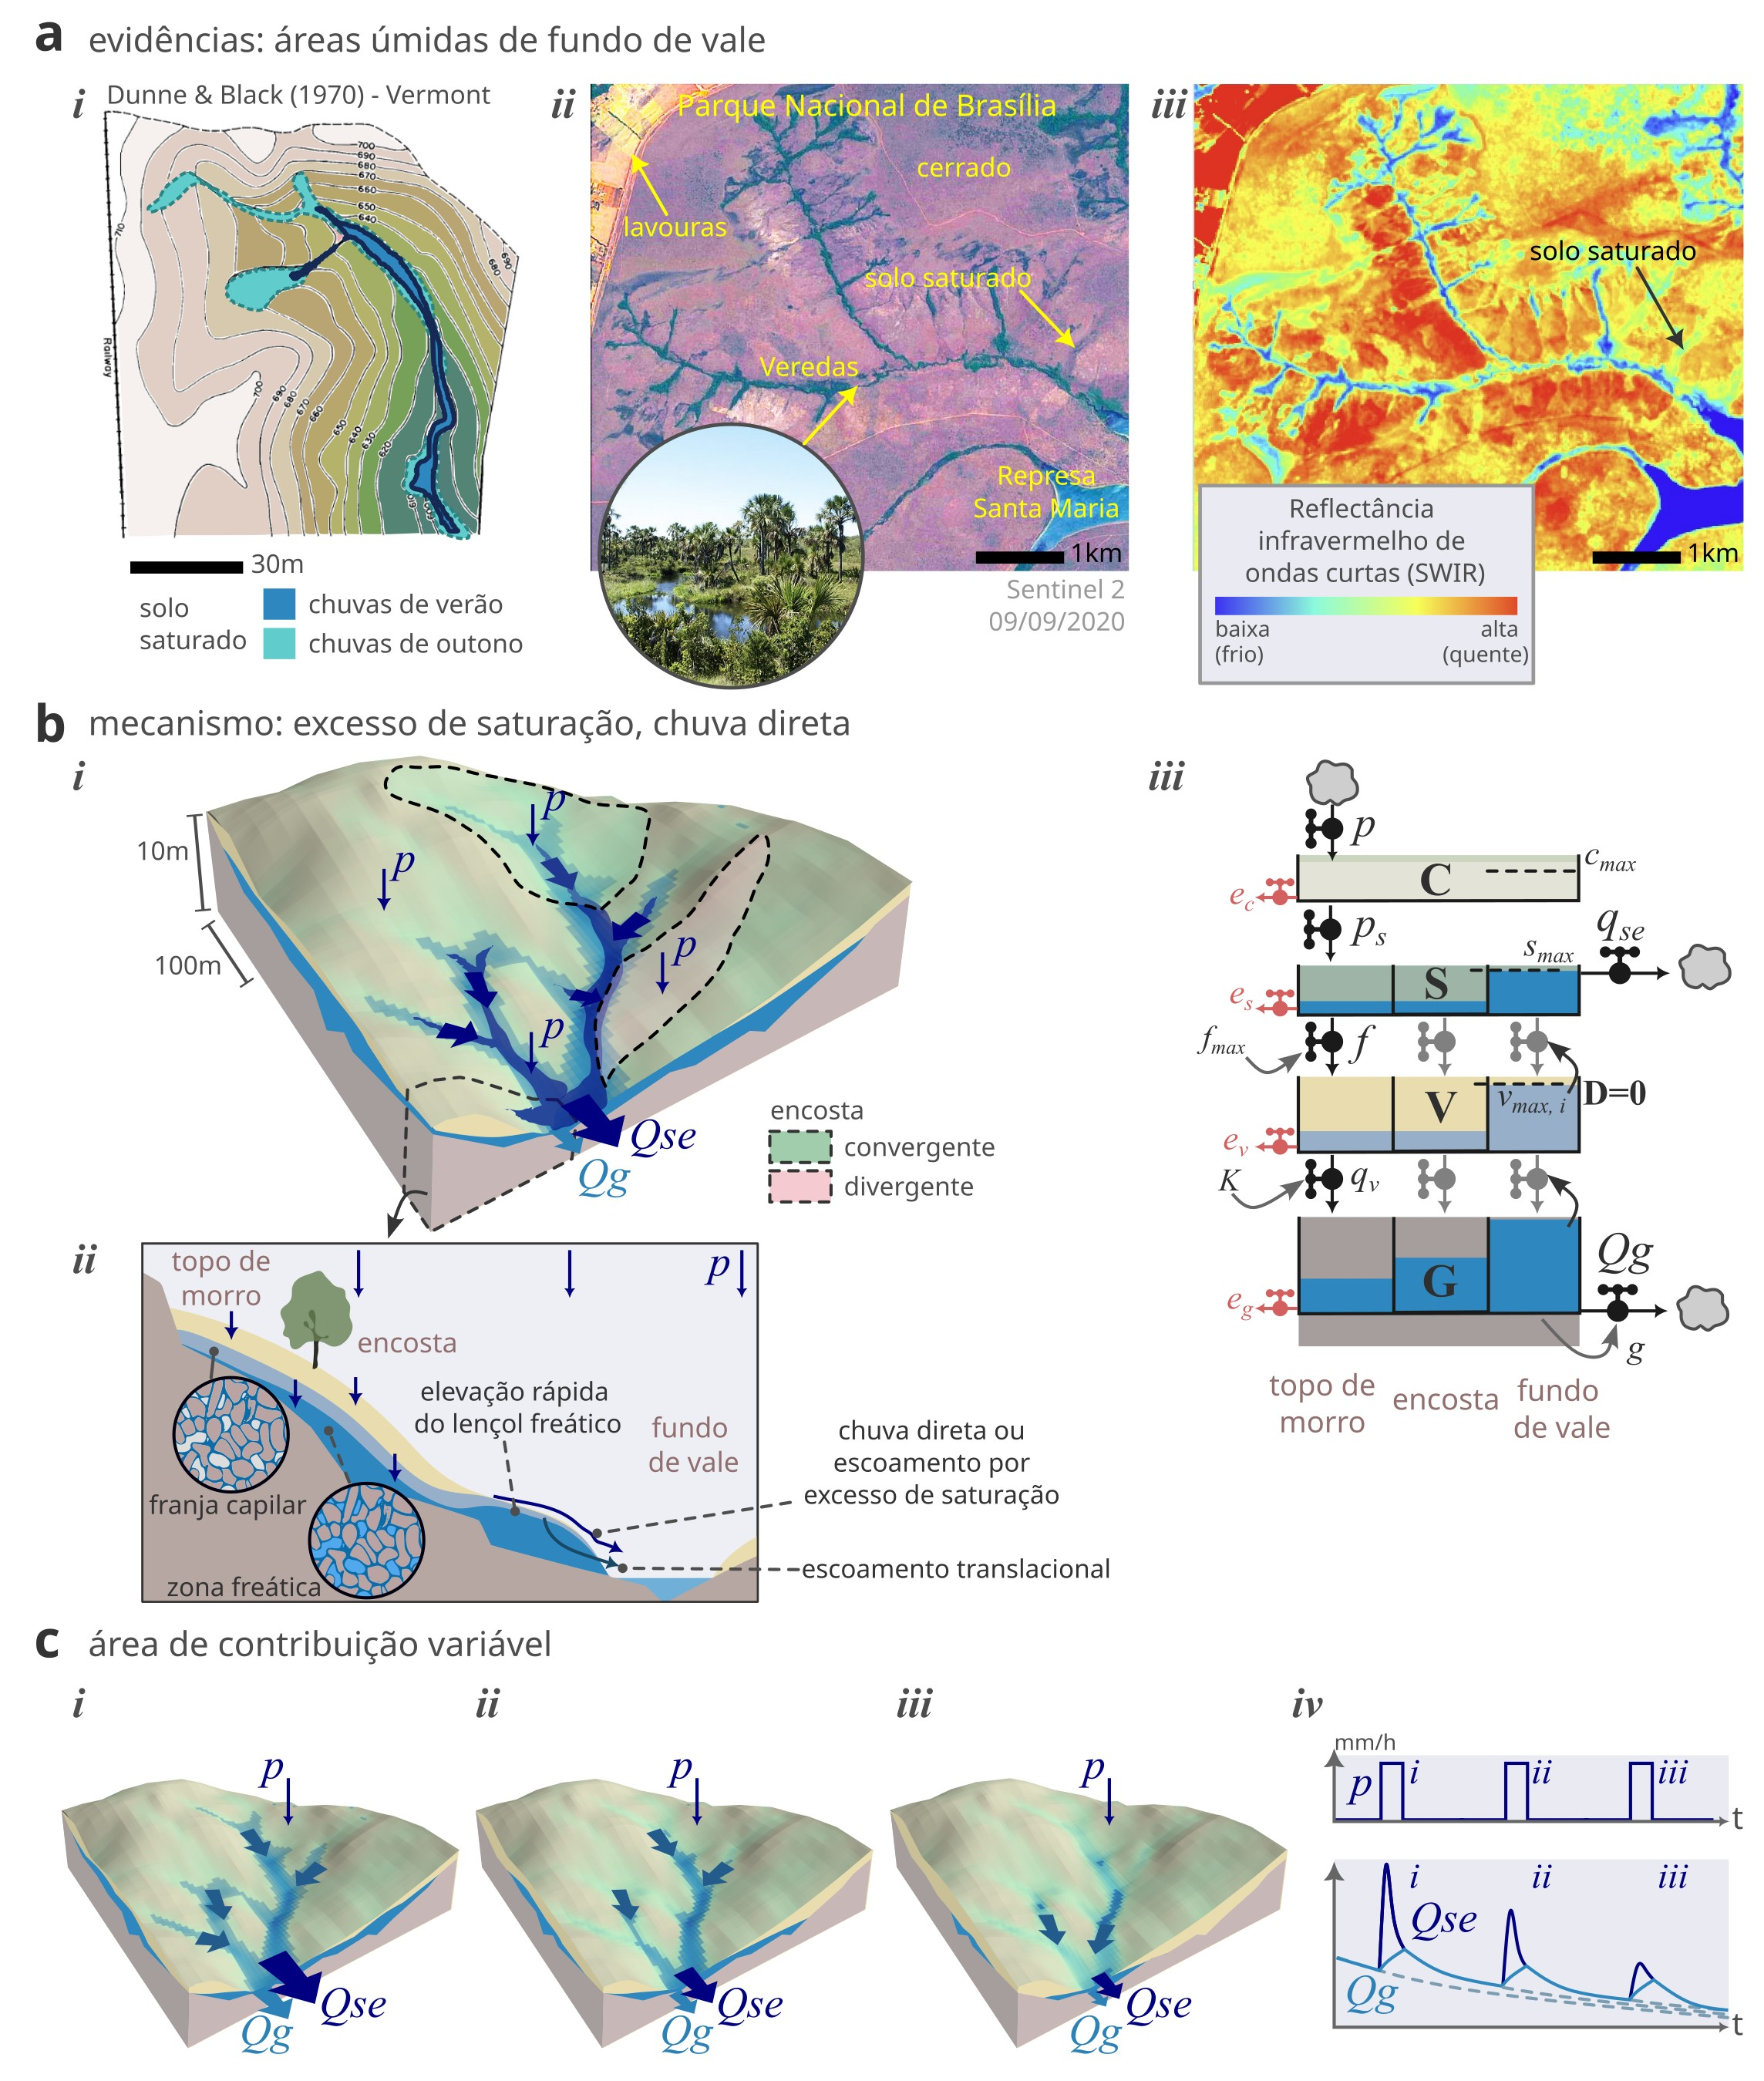
\includegraphics[width=0.98\linewidth]{figs/fig_topo.jpg}		
\caption[A topografia e a área de contribuição variável]
{\textbf{---\;A topografia e a \gls{vsa}.}
    A topografia exerce um controle crucial na formação de \gls{sat_areas} que variam de extensão durante as chuvas e ao longo das estações. Essas áreas de solo saturado, assim, produzem \gls{rse}, além de respostas subterrâneas rápidas por \gls{trans_flow}.
    \;\textbf{a}\;---\;Evidências: mapa de Dunne \& Black (1970) em Vermont (Estados Unidos), demonstrando a extensão das \gls{sat_areas} em épocas distintas do ano (detalhe \textrm{\textit{i}}), e; Veredas úmidas na estação seca no Parque Nacional de Brasília, observadas pela reflectância no infravermelho de ondas curtas de uma cena Sentinel-II em 9 de Setembro de 2020 (detalhes \textrm{\textit{ii}} e \textrm{\textit{ii}}). 
    \;\textbf{b}\;---\;Sistematização do mecanismo de escoamento por excesso de saturação. O solo das partes da bacia (fundo de vale, encosta e topo de morro) saturam-se em velocidades diferentes, gerando respostas rápidas principalmente nos fundos de vale. Encostas convergentes tendem a produzir mais \gls{rse} do que \gls{spurs}, onde predomina a \gls{qv} e o \gls{ground-flow}.
    \;\textbf{c}\;---\;Esquematização da retração das \gls{sat_areas} ao longo de uma estiagem (dinâmica sazonal). Esse processo também apresenta uma dinâmica efêmera, durante e logo após eventos de chuva. Fonte da fotografia em \textbf{b}: https://commons.wikimedia.org/wiki/File:Veredas.jpg .
}
\label{fig:hydro:topo} 		
\end{figure}

\par O \gls{paradigma} Hortoniano não foi apenas refutado pela constatação da \gls{subsur_flow}, pois evidências empíricas também acumularam-se para sustentar a existência de mais dois mecanismos de resposta rápida, menos intuitivos, que ocorrem em \textbf{\gls{sat_areas}}. Esses mecanismos, ilustrados na Figura \ref{fig:hydro:topo}, resultam da interação da chuva com um lençol freático raso e dinâmico, sendo um o \gls{rse}, e o outro o \gls{trans_flow} (detalhes na próxima seção). Ambos estão relacionados entre si, são fortemente controlados pela topografia do terreno e também produzem consequências sobre a manifestação da \gls{subsur_flow} em macroporos, como veremos adiante. O primeiro deles surge na literatura quando a precipitação direta na área do entorno de canais e nascentes é citada por Hursh \& Brater (1941) \cite{Hursh1941} como umas das fontes de escoamento fluvial nas bacias da Floresta Experimental de Coweeta:   

\begin{adjustwidth}{100pt}{0pt}
\medskip
\small Contribuições de áreas com lençóis freáticos normalmente rasos, localizadas próximas ao riacho e ocorrendo em perfis de solo que se saturam rapidamente. Onde tais condições ocorrem ao longo de um riacho, espera-se um aumento real na largura do canal e, consequentemente, um aumento na quantidade de precipitação direta sobre o canal. Áreas com lençóis freáticos altos adjacentes a nascentes também são esperadas para contribuir de forma semelhante.\footnote{Tradução livre de: \textit{Contributions from areas of normally shallow water-tables located in close proximity to the stream, and occurring in soil-profiles which are quickly saturated. Where such conditions occur along a stream, it is expected that there will be an actual increase in the width of the channel and subsequent increase in the amount of channel-precipitation. Areas of high water tables adjacent to spring-heads would be expected to contribute similarly.}} -- Hursh \& Brater (1941, p. 870) \cite{Hursh1941}.
\medskip
\end{adjustwidth}

\noindent Essa é certamente uma das descrições pioneiras do conceito de \textbf{\gls{vsa}}: a geração de \gls{sf-runoff} em função da \textit{expansão e retração de áreas úmidas} nos fundos de vale, juntos aos riachos. Esse mecanismo, ilustrado na Figura \ref{fig:hydro:topo}\textbf{c}, permite que qualquer \gls{ground-rain} transforme-se em uma \gls{ex-rain} quando precipitada sobre áreas com solo saturado, fato que ajuda a explicar a prevalência de enchentes mesmo em bacias com solos de alta \gls{infmax} (como no caso de La Grange Brooke, perto de onde Robert Horton morava \cite{Beven2004c}). Esse conceito foi bem organizado por Cappus (1960) \cite{Cappus1960} em um estudo na Bacia Experimental de Alrance (315 ha, França). O autor alegou ter evidências para uma \say{nova \gls{teoria} de escoamento superficial}, em que a área da bacia pode ser separada por uma \textit{zona de escoamento superficial} e uma \textit{zona de infiltração}. A primeira delas inclui uma parte \textit{fixa} de áreas impermeáveis e outra parte \textit{variável} de áreas permeáveis, mas que estão com o solo saturado:

\begin{adjustwidth}{100pt}{0pt}
\medskip
\small
A bacia experimental pode ser dividida em duas zonas \(S_r\) e \(S_i\) de extensões variáveis: --- A zona de enxurradas \(S_r\) de área \(A_r\) inclui, por um lado, zonas impermeáveis de extensão fixa (estradas, caminhos pavimentados, caminhos de terra compactada pelo tráfego repetido de pessoas ou gado, superfícies rochosas, etc.) e, por outro lado, zonas de extensão variável constituídas por terrenos permeáveis, mas quase completamente saturados de água. A chuva que cai na zona \(S_r\) se transforma inteiramente em \gls{sf-runoff} ou escoamento subsuperficial. --- A zona de infiltração \(S_i\) de área \(A_i\) é constituída por terrenos permeáveis não saturados. O solo de textura arenosa, que forma as camadas superficiais da bacia experimental, é caracterizado por uma \gls{infmax} \(f\) muito alta que excede a intensidade de todas as chuvas que podem cair sobre esta bacia — exceto apenas por chuvas de uma raridade extrema. Assim, salvo em casos muito excepcionais, a chuva que cai na zona \(S_i\) é completamente absorvida por infiltração e, consequentemente, não gera nenhum escoamento.
\footnote{Tradução livre de: 
\textit{
Le Bassin expérimental peut être partagé en deux zones $S_r$ et $S_i$ d'étendues variables:\;--- La zone de ruissellement $S_r$ de superficie $A_r$ comporte, d'une part, des zones imperméables d'étendue fixe (routes, chemins empierrés, chemins de terre tassée par le passage répété des hommes ou du bétail, surfaces rocheuses, etc.) et, d'autre part, des zones d'étendue variable constituées de terrains perméables, mais à peu près complètement saturés d'eau. La pluie tombant sur la zone Sr se transforme entièrement en ruissellement superficiel ou hypodermique. --- La zone d'infiltration $S_i$ de superficie $A_i$ est constituée par les terrains perméables non saturés. Le sol de texture sableuse, qui forme les couches superficielles du Bassin expérimental est caractérisé par une capacité d'infiltration $f$ très forte qui dépasse l'intensité de toutes les pluies pouvant tomber sur ce bassin — à l'exception seulement de pluies d'une rareté extrême — ainsi, sauf en des cas très exceptionnels, la pluie tombant sur la zone $S_i$ est entièrement absorbée par infiltration et ne donne lieu par conséquent à aucun ruissellement.
}} -- Cappus (1960, p. 503) \cite{Cappus1960}.
\medskip
\end{adjustwidth}

\noindent Tsukamoto (1963) \cite{Tsukamoto1963} também estruturou uma \gls{teoria} semelhante, alicerçado nos resultados obtidos em uma bacia na Floresta da Universidade de Tóquio (106,7 ha, Japão). No seu artigo, ele aponta que as áreas ripárias manifestam respostas de saturação rápidas devido à influência da \textbf{\gls{fringe}} da água subterrânea, gerando \gls{sf-runoff} nessa parte da encosta, em oposição às partes mais altas e bem drenadas do terreno. Os resultados experimentais de Ragan (1968) \cite{Ragan1968}, mencionados acima, também demonstraram elevações rápidas do lençol freático perto do riacho durante os eventos de chuva monitorados. Mesmo Betson (1964) \cite{Betson1964}, ainda que tente sustentar o \gls{percept-model} Hortoniano, não deixou de comentar que metade do escoamento possivelmente foi gerado por uma área pantanosa em uma das bacias analisadas em seu estudo.

\par Com o objetivo de corroborar a \gls{teoria} da \gls{vsa}, Dunne \& Black (1970) \cite{Dunne1970, Dunne1970b} publicaram resultados detalhados para uma pequena bacia experimental em Vermont (Estados Unidos). Nesse estudo, os autores exibem mapas das áreas de solo saturado que acompanham o talvegue do terreno (detalhe \textit{i} na Figura \ref{fig:hydro:topo}\textbf{a}), mas que manifestaram variações tanto ao longo do ano (dinâmica sazonal) quando durante os eventos de chuva (dinâmica efêmera). A dinâmica sazonal dessas áreas úmidas explica-se pelo aumento da \gls{qv} da água subterrânea durante a estação mais úmida, fato que aumenta a extensão das zonas de afloramento de nascentes nos fundos dos vales. O detalhe \textit{ii} na Figura \ref{fig:hydro:topo}\textbf{a} demonstra evidências da dinâmica sazonal a partir da reflectância do infravermelho de ondas curtas (\texttt{SWIR}) com uma cena Sentinel-II em 9 de Setembro de 2020, no Parque Nacional de Brasília. Essa época é marcada pela estiagem, mas as áreas ripárias permanecem úmidas, formando as Veredas. Por outro lado, a dinâmica efêmera explica-se por um processo de rápido de elevação da \gls{sat-zone} quando a \gls{fringe} está muito próxima da superfície (mais detalhes adiante)\footnote{Fenômeno descrito em inglês por \textit{groundwater ridging}.}. 

\par A constatação inequívoca da dinâmica das áreas saturadas por Dunne \& Black (1970) consolidou a percepção de que a \textit{topografia} exerce um controle importante na \gls{hydrology} de bacias de ordem zero, e não apenas a \textit{superfície} do solo, como postulado pelo \gls{paradigma} da infiltração. Nesse sentido, Anderson \& Burt (1978) \cite{Anderson1978} demonstram que, em uma bacia em Quantock Hills (Inglaterra), a elevação rápida do lençol freático pelos talvegues das \textbf{\gls{hollows}}\footnote{Tradução livre de \textit{hollow}.} é muito maior que nas \textbf{\gls{spurs}}\footnote{Tradução livre de \textit{spur}.}. As primeiras, assim, tendem a gerar relativamente mais \gls{rse} e também mais \gls{subsur_flow}, pois a elevação súbita da água subterrânea ativa a rede de macroporos no solo. Nas \gls{spurs}, por outro, predominam os processos mais lentos de \gls{qv} e \gls{ground-flow}. lado Diante disso, o mecanismo de \gls{sf-runoff} defendido na \gls{teoria} de Horton (excesso de infiltração) não foi exatamente refutado, mas reservado como um mecanismo de resposta restrito a eventos extraordinários de precipitação ou a zonas com solo alterado, seja em ambientes naturais (como em afloramentos rochosos e regiões áridas), seja em ambientes antropizados (como na agricultura e áreas urbanas)\footnote{Isso implica que o emprego do método \acrshort{cn} do \acrshort{scs} é justificado quando a sua aplicação é voltada para eventos extremos de chuva ou em bacias urbanas e rurais em que o mecanismo Hortoniano é claramente dominante. No entanto, essa restrição não é explícita nos manuais oficiais do método, que incluem também valores de \acrshort{cn} para florestas e outras cobertura do solo naturais. Além disso, modelos de simulação como \texttt{SWAT} e \texttt{SWMM} fazem uso de simulação contínua (eventos de chuva diversos) e representam qualquer cobertura do solo.}. Cabe destacar que Horton (1936) \cite{Horton1936} chegou perto de deduzir analiticamente esse mecanismo em um de seus artigos, pois ele destaca o fato de que encostas de solo com soleiras inclinadas induzem o lençol freático a interceptar a superfície do terreno acima do nível do fundo do vale, causando o surgimento de uma superfície saturada nessa parte convergente da topografia \cite{Beven2004b}.

\subsection{Paradoxos}

\begin{figure}[t!] 
\centering				
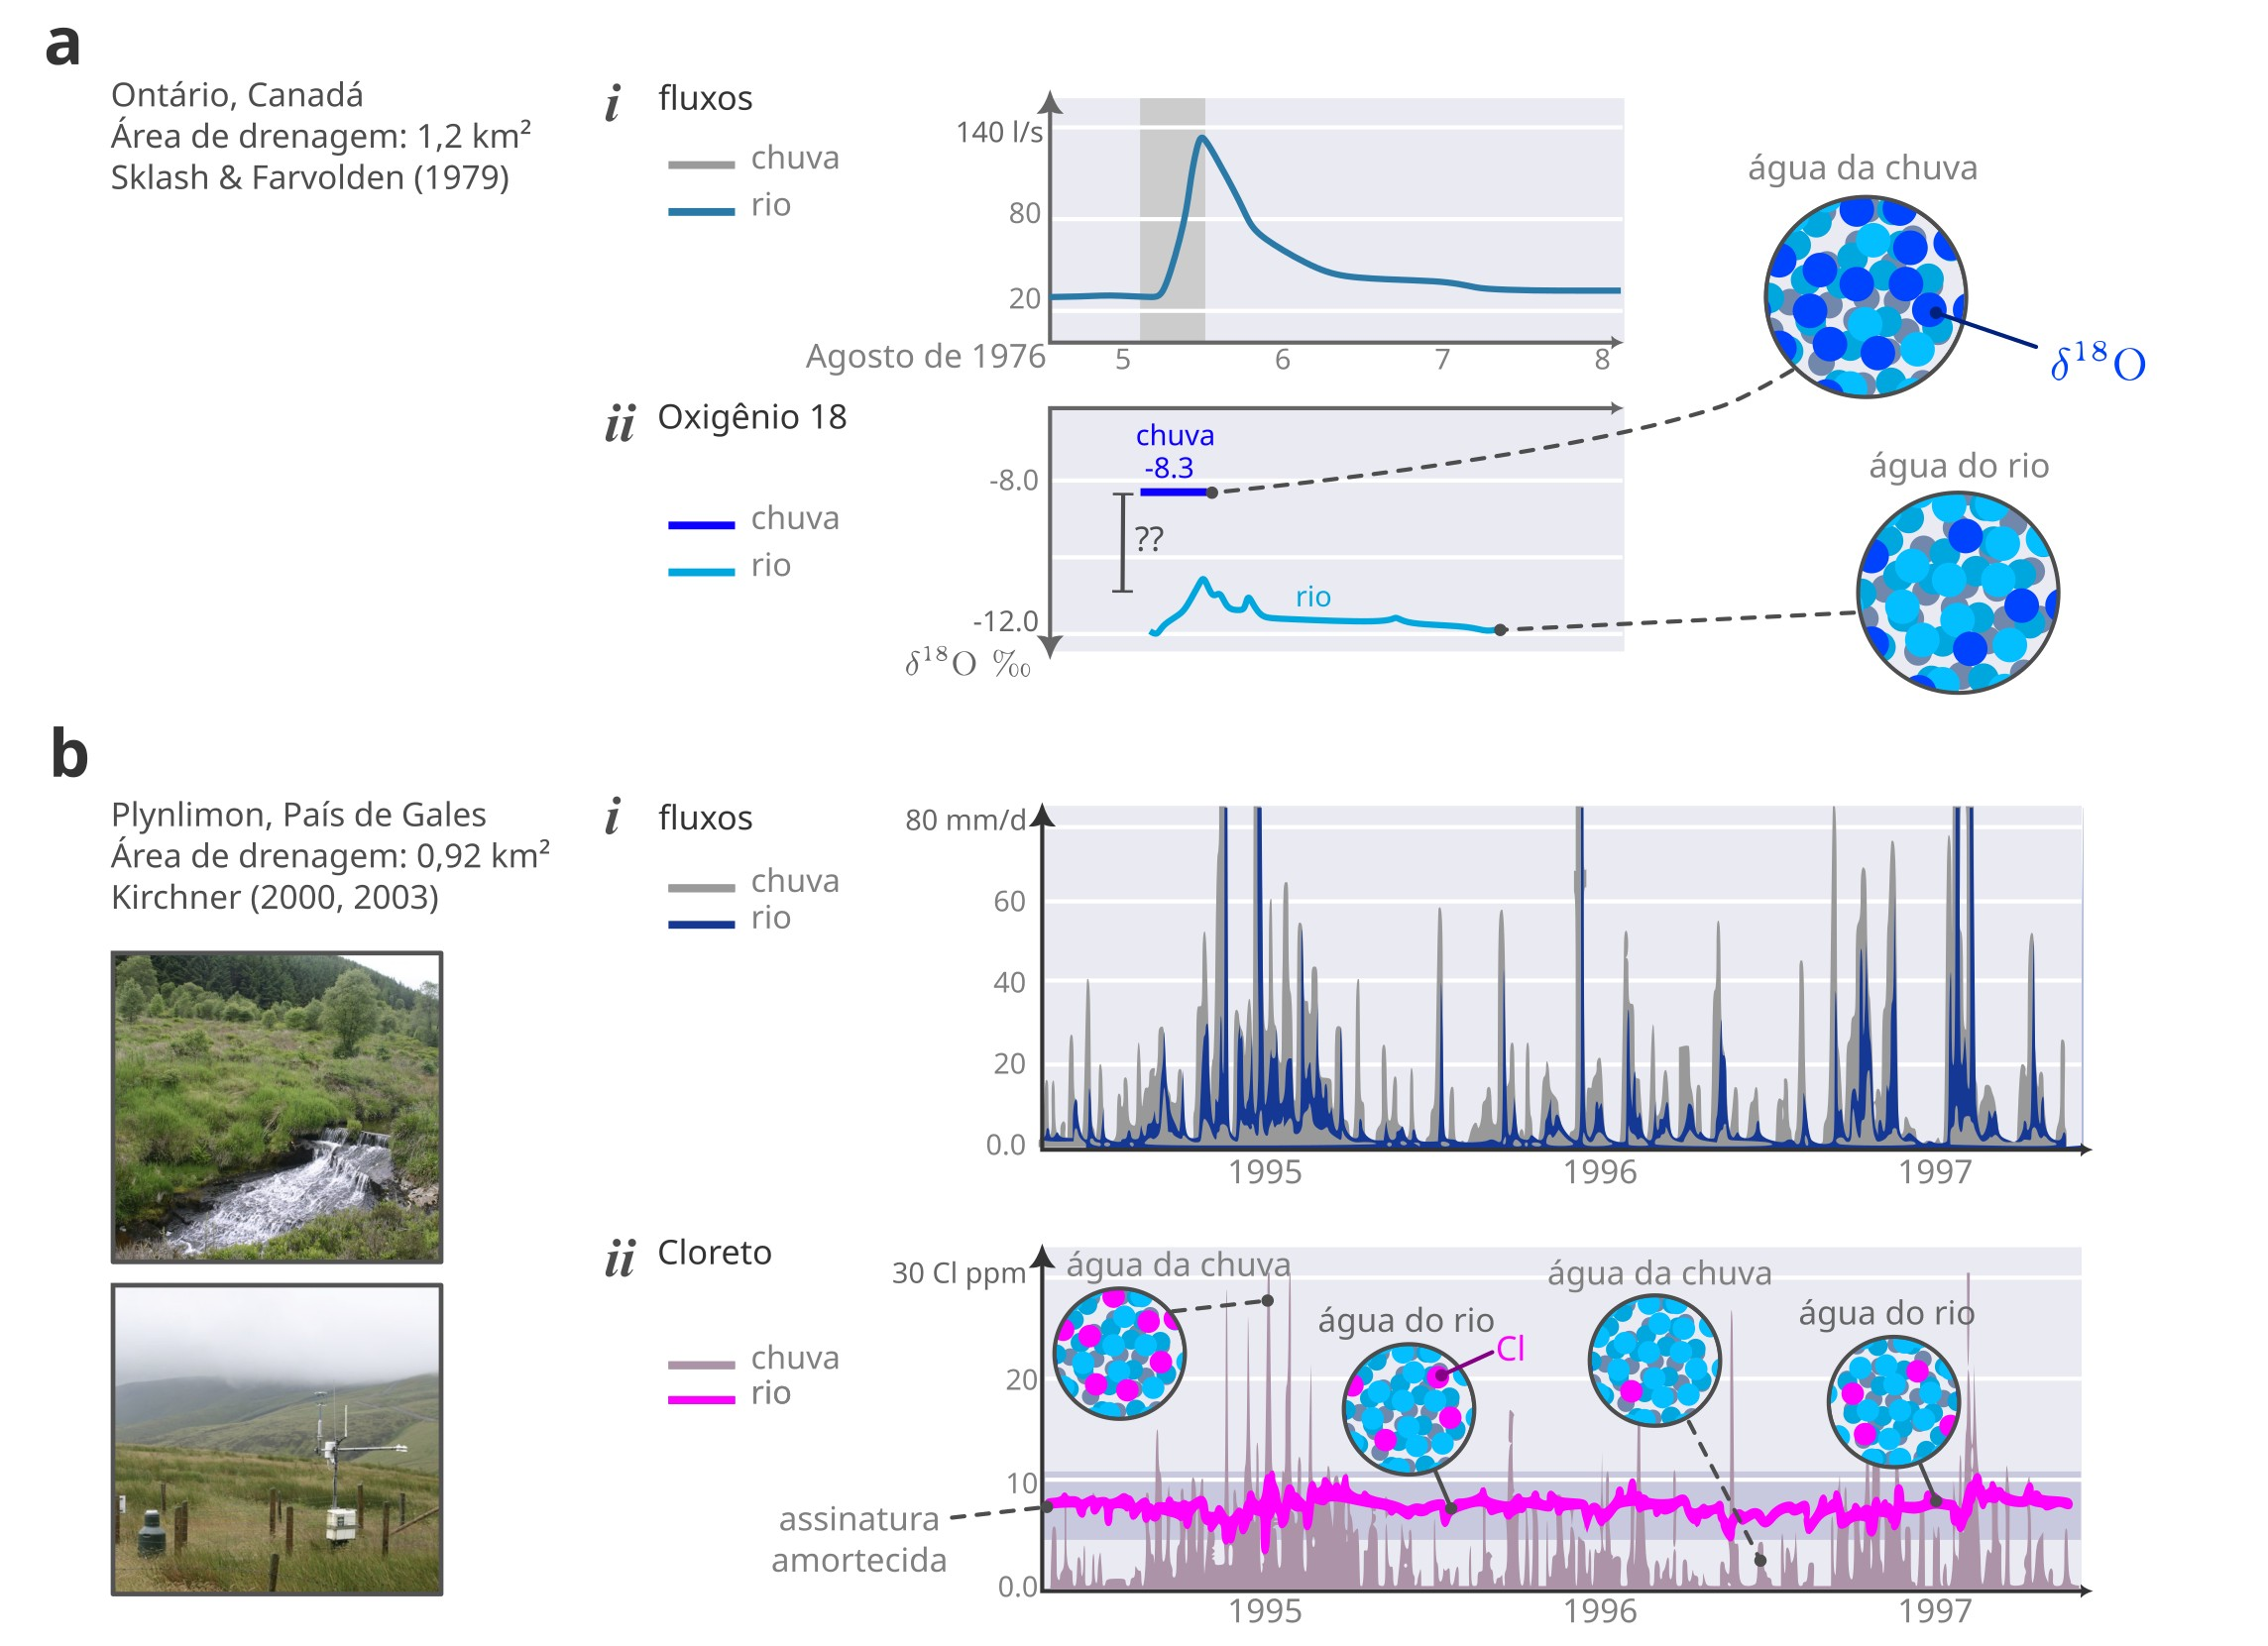
\includegraphics[width=0.98\linewidth]{figs/fig_paradox2.jpg}		
\caption[O paradoxo da água velha]
{\textbf{---\;O \gls{old_water_paradox}.}
    Análises da \gls{iso_sign} e geoquímica da água da chuva e do rio durante enchentes deixam claro que são águas com idades diferentes, criando assim um paradoxo. \;\textbf{a}\;---\;Evidências trazidas por Sklash \& Farvolden (1979) \cite{sklash1979} em uma bacia rural em Ontário, Canadá (1,2 km² de área de drenagem). Os fluxos claramente denotam uma resposta rápida da bacia (enchente) diante do evento de chuva (detalhe \textrm{\textit{i}}). Mas a \gls{iso_sign} com Oxigênio-18 evidencia que a água na enchente não é a mesma água da chuva (detalhe \textrm{\textit{ii}}).\;\textbf{b}\;---\;O mesmo paradoxo verificado com Cloreto (aerossol marinho) por Kirchner et \textit{al.} (2000, 2003) \cite{kirchner2000, Kirchner2003} em uma bacia experimental em Plynlimon, no País de Gales (0,92 km² de área de drenagem). os fluxos são típicas respostas rápidas (detalhe \textrm{\textit{i}}), mas a assinatura do rio apresenta um amortecimento pronunciado ao longo dos anos, sugerindo uma mistura de longa duração (detalhe \textrm{\textit{ii}}). Fonte das fotografias: Ecological Continuity Trust \cite{ect_plynlimon}.
}
\label{fig:hydro:paradox2} 		
\end{figure}

\par O escoamento subterrâneo translacional, por sua vez, é especulado conceitualmente por Hewlett \& Hibbert (1967) \cite{Hewlett1967}, em um artigo claramente revolucionário no campo da \gls{hydrology} \cite{McDonnell2009}. Ao mesmo tempo que criticam o \gls{paradigma} hegemônico da época (a \gls{teoria} da capacidade de infiltração), os autores organizam novos conceitos relevantes, como os termos \say{respostas rápidas e lentas} e \say{área de contribuição variável}, pavimentando o caminho para o advento do novo \gls{paradigma}. Nessa direção, os autores sugerem um mecanismo de resposta subterrânea \textit{instantânea} que ocorreria quando a \gls{fmc} do solo é superada pela infiltração da água da chuva nas zonas ripárias, onde há maior influência das franjas de capilaridade. Em resumo, eles postulam que essa resposta, ainda que rápida, não seria exatamente a água da chuva, mas água que se alojou na matriz do solo \textit{antes} do evento ocorrer. Nesse processo, a espessura dos filmes de águas nas partículas do solo na \gls{unsat-zone} atingem subitamente um limite em que a rede de poros torna-se pressurizada pela gravidade. Por isso, a \textbf{água nova} da chuva (água do evento) desencadeia um pulso, uma onda de pressão, que expele a água armazenada no solo na base da encosta, uma \textbf{água velha} (água pré-evento):

\begin{adjustwidth}{100pt}{0pt}
\medskip
\small
No entanto, da parte que contribui para o escoamento, uma fração será de algumas das gotas que literalmente caíram durante a tempestade -- ou seja, um pouco de chuva nova -- e a outra fração será o que podemos chamar de \textit{fluxo translacional}, ou fluxo produzido por um processo de substituição. Esta é uma contribuição para o escoamento de água já armazenada no manto do solo antes do início da chuva. Ela será liberada em grandes quantidades apenas quando o solo estiver dentro da faixa de \gls{fmc} ou mais úmido. Acima da \gls{sat-zone}, podemos considerar esse movimento como devido ao espessamento dos filmes de água que envolvem as partículas do solo e a um pulso resultante de fluxo de água à medida que a saturação ocorre.
\footnote{Tradução livre de: 
\textit{
However, of the part contributed to direct runoff, a fraction will be some of the actual drops that fell during the storm -- that is, some new rain -- and the other fraction will be what we might call translatory flow, or flow produced by a process of displacement. This is a contribution to direct flow of water already stored in the soil mantle before rainfall began. It will be released in large quantities only when the soil is within field capacity range or wetter. Above the zone of saturation, we may regard such movement as due to thickening of the water films surrounding soil particles and a resulting pulse of water flux as the saturated zone is approached.
}} -- Hewlett \& Hibbert (1967, p. 279) \cite{Hewlett1967}.
\medskip
\end{adjustwidth}

\par Ainda que a \gls{teoria} faça sentido e cite estudos em laboratório, o texto de Hewlett \& Hibbert (1967) não oferece evidências empíricas obtidas em campo para justificar a realidade desse mecanismo. Mas isso deixou de ser uma lacuna a partir de Pinder e Jones (1969) \cite{pinder1969}, que avaliaram a separação do hidrograma de enchentes em três bacias monitoradas na Nova Escócia (entre 647,5 ha a 13,5 km², Canadá). Ao contrário dos métodos gráficos convencionais, eles inferiram a separação entre \gls{sf-runoff} e escoamento subterrâneo com marcadores químicos e um \gls{model} simples de balanço de massa\footnote{O \gls{model} desenvolvido consiste em dois compartimentos de mistura: $C_{tr}Q_{tr} =C_{dr}Q_{dr} + C_{gw}Q_{gw}$, em que: $C$ é a concentração de algum soluto conservativo; $Q$ é a vazão; $tr$ denota vazão total; $dr$ denota o escoamento direto, e; $gw$ denota o escoamento subterrâneo.}. No caso apresentando, foram monitoradas as concentrações de sódio, cálcio, bicarbonato, magnésio e sulfato antes e durante os eventos de enchentes. Os resultados indicaram uma prevalência substancial de escoamento subterrâneo durante as enchentes, com 32\% a 42\% da vazão máxima do hidrograma. Isso, porém, não eliminava a explicação alternativa de uma resposta subsuperficial da água da chuva (água nova) que dissolvera os solutos monitorados ao transitar rapidamente pelo solo. Evidências a favor da água subterrânea (água velha) tornarem-se muito mais robustas com o advento do monitoramento de isótopos de hidrogênio e oxigênio, como Deutério ($^{2}\text{H}$), Trítio ($^{3}\text{H}$) e Oxigênio-18 ($^{18}\text{O}$), marcadores ideais que fazem parte da própria molécula de água\footnote{Ao contrário de solutos comuns, a concentração de $^{18}\text{O}$ é medida pela diferença em partes por mil ($\delta^{18}\text{O}$ \textperthousand) da razão de $^{18}\text{O}/^{16}\text{O}$ de um padrão e a amostra: $\delta^{18}\text{O} = (\frac{^{18}\text{O}/^{16}\text{O} \,\text{amostra}}{^{18}\text{O}/^{16}\text{O}\,\text{padrão}} - 1) \times 1000$. O padrão costuma ser a água média dos oceanos (\texttt{SMOW} -- \textit{Sea Mean Ocean Water}). Águas desprovidas de $^{18}\text{O}$ em relação ao padrão exibem $\delta^{18}\text{O}$ negativo, e vice-versa.}. Em locais com grande variabilidade na \textbf{\gls{iso_sign}} da água precipitada, é possível se estimar o quanto dessa água nova se faz presente durante as enchentes\footnote{Obviamente, se a água da chuva for indistinguível em termos isotópicos da água no rio logo antes do evento, então é impossível extrair alguma informação relevante.}. Essa estratégia foi sugerida por Dinçer et \textit{al.} (1970) \cite{dincer1970} em um estudo nas montanhas da Tchecoslováquia que demonstrou o efeito do \textbf{\gls{term_frac}}\footnote{A principal causa da fracionamento desses isótopos na atmosfera decorre da diferença de pressão de vapor entre moléculas de água isotopicamente pesadas e leves: ${\text{H}_{2}}^{18}\text{O}$ tem uma pressão de vapor mais baixa do que  ${\text{H}_{2}}^{16}\text{O}$ e, portanto, ${\text{H}_{2}}^{16}\text{O}$ permanece preferencialmente na fase líquida tanto nos processos de evaporação quanto de condensação. Por isso, as concentrações observadas de $\delta^{18}\text{O}$ na precipitação tendem a ser incrementalmente negativas à medida que as massas de ar úmido avançam sobre os continentes \cite{sklash1976}.} nas concentrações de $^{3}\text{H}$ e $^{18}\text{O}$ em camadas de neve precipitadas e derretidas ao longo das estações. A seguir, os resultados publicados por Martinec et \textit{al.} (1974) \cite{martinec1974} notam que a água de rios nas montanhas da Suíça exibia uma concentração de $^{18}\text{O}$ com variabilidade relativamente baixa, que se aproximava da média de longo prazo das oscilações sazonais observadas na precipitação. A estratégia então assumiu contornos bem definidos com o artigo de Sklash et \textit{al.} (1976) \cite{sklash1976}, que além de organizar a lógica do método, mostra que em duas bacias monitoradas em Ontário (Canadá), a contribuição da água subterrânea na vazão máxima das enchentes foi entre 55\% (em bacias de montante) até 70\% (nas bacias de jusante, drenando uma área de 700 km$^2$). São resultados com conotações revolucionárias:

\begin{adjustwidth}{100pt}{0pt}
\medskip
\small
A descoberta mais importante é que a componente pré-evento da enchente de 16 de Maio foi grande. Por exemplo, no pico da vazão total, a componente pré-evento do arroio Big Otter em Viena foi de 70 $\pm$ 9\% do escoamento da enchente. Esses resultados substanciam as descobertas de Pinder \& Jones (1969) e Fritz et \textit{al.} (1974), embora as bacias no presente estudo sejam de uma a duas ordens de magnitude maiores em extensão de área. Esses resultados não são consistentes com os resultados simulados de Freeze (1972b), os resultados de campo de Dunne \& Black (1970a,b), e Hewlett \& Hibbert (1967), ou as implicações teóricas de Horton (1933). Os resultados são particularmente encorajadores, no entanto, à luz da grande componente subsuperficial (pré-evento) do derretimento da neve observado por Dinçer et \textit{al.} (1970).
\footnote{Tradução livre de: 
\textit{
The most important finding is that the pre-storm component of storm runoff for the 16 May storm was large. For example, at peak total discharge, the pre-storm component of Big Otter Creek at Vienna was 70 $\pm$ 9\% of storm runoff. These results substantiate the findings of Pinder \& Jones (1969) and Fritz et al. (1974), even though the basins in the present study are one to two orders of magnitude larger in areal extent.These results are not consistent with the simulated results of Freeze (1972b), the field results of Dunne \& Black (1970a,b), and Hewlett \& Hibbert (1967), or the theoretical implications of Horton (1933). The results are particularly encouraging, though, in light of the large subsurface (prestorm) component of snowmelt noted by Dinçer et al. (1970).
}} -- Sklash et \textit{al.} (1976, p. 276) \cite{sklash1976}.
\medskip
\end{adjustwidth}

\noindent Michael Sklash prosseguiu com estudos desse tipo, corroborando a existência desse processo em bacias no Canadá, na Nova Zelândia e nas Ilhas Britânicas \cite{sklash1979, sklash1986, sklash1996}. Por exemplo, o artigo de Sklash \& Farvolden (1979) \cite{sklash1979}, no Canadá, traz resultados semelhantes para uma bacia com agricultura intensiva (1,2 km$^2$, na Bacia Experimental Hillman Creek, Ontário, Figura \ref{fig:hydro:paradox2}\textbf{a}) e duas bacias altamente florestadas (1,0 km$^2$ e 3,9 km$^2$, Bacia Experimental Ruisseau des Eaux Volées, Québec). Além de reportar a prevalência surpreendente da água velha nas enchentes (entre 80\% a 94\% to total escoado), os autores alimentam a \gls{teoria} das subidas rápidas da água subterrânea nos fundos de vale para explicar o fenômeno. Na Bacia Experimental de MaiMai (Nova Zelândia), Sklash et \textit{al.} (1986) \cite{sklash1986} trazem resultados que revisam drasticamente as interpretações de Mosley (1979) \cite{Mosley1979}. Citado acima, Mosley (1979) argumenta sobre a dominância nessa bacia da \gls{subsur_flow} (água nova). A prevalência inequívoca de água velha nas enchentes, obtida com os marcadores isotópicos, trouxe um certo impasse na \gls{comunidade-cientifica}, que passou desde então a propor mecanismos plausíveis \cite{buttle1994}. Nesse contexto, McDonnell (1990) \cite{mcdonnell1990} faz uma síntese dos mecanismos de resposta na bacia de MaiMai, trazendo o conceito de \textbf{ativação do escoamento subterrâneo} a partir da entrada da água da chuva na rede de macroporos das encostas, ou seja, pela \gls{subsur_flow}. Nesse esquema (ilustrado na Figura \ref{fig:hydro:paradox}\textbf{a}), ele ressalta o papel de atalhos \textit{verticais} no perfil do solo, criado por macroporos, que fazem a água nova da chuva rapidamente se alojar nas franjas capilares da \gls{sat-zone}, criando então a ativação da carga hidráulica necessária para expulsar rapidamente a água subterrânea velha na base da encosta. Uma nova revisão, trazida por McGlynn et \textit{al.} (2002) \cite{mcglynn2002}, apresenta também o efeito relevante da \textbf{\gls{bedrock_topo}} da encosta (o embasamento de rocha relativamente impermeável). Sugere-se que as irregularidades dessa camada podem criar \textbf{zonas de estagnação}, ou \textbf{bolsões}, que armazenam a água no subsolo por tempos muito mais longos que o esperado. A eventual ativação hidráulica dessas partes relativamente inacessíveis expelem água velha na base da encosta, facilitada pela presença de macroporos. De fato, a influência das estruturas geológicas subjacentes (fraturas) no afloramento da água subterrânea já eram mencionadas por Huff et \textit{al.} (1982) \cite{Huff1982}, mas sem a análise da idade da água com isótopos.

\begin{figure}[t!] 
\centering				
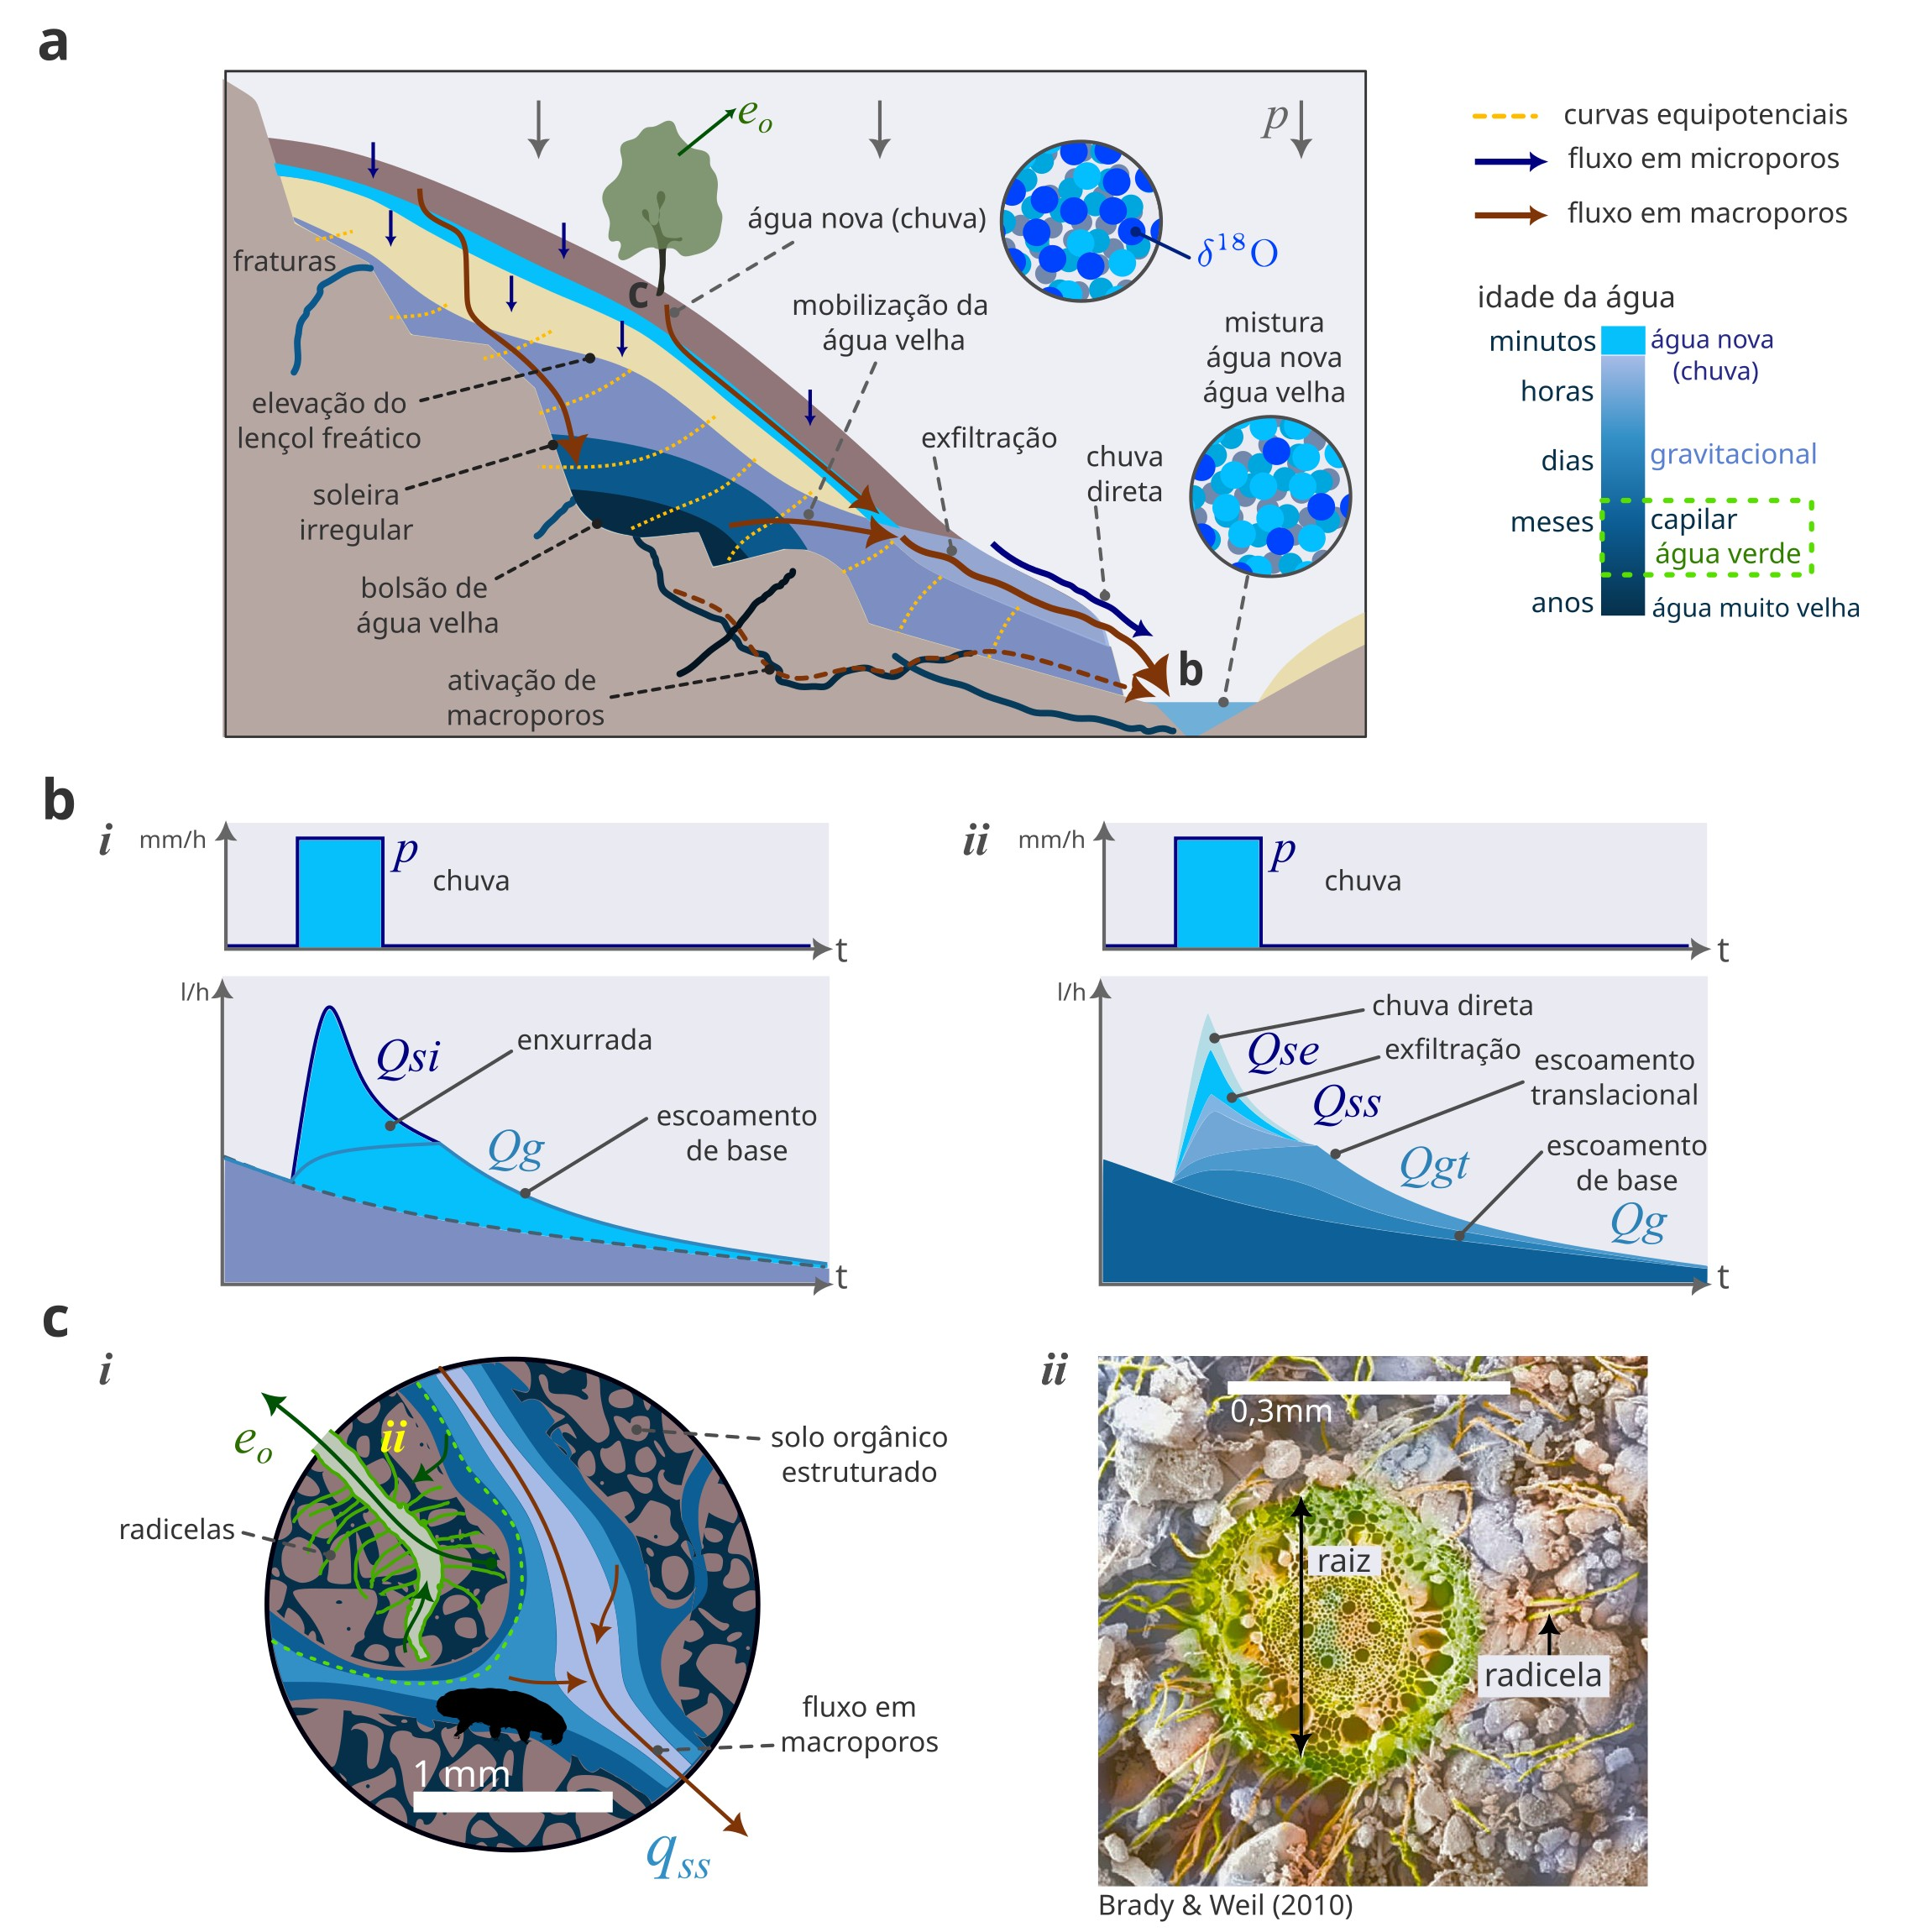
\includegraphics[width=0.98\linewidth]{figs/fig_paradox.jpg}		
\caption[Mobilização da água velha]
{\textbf{---\;Mobilização da água velha.}\;\textbf{a}\;---\;A elevação do lençol freático combinada com o fluxo por macroporos (fraturas e caminhos preferenciais) ajudam a explicar a dominância de água velha nas respostas rápidas dos rios. Atalhos verticais permitirem que água nova (chuva) se misture com água mais velha em zonas estagnadas (bolsões) na soleira do aquífero, ativando a carga hidráulica em fraturas e caminhos preferenciais, fato que resulta na a expulsão rápida da água velha.\;\textbf{b}\;---\;Diferenças entre o \gls{model} Hortoniano de resposta rápida (enchente Tipo 3) e o \gls{model} obtido a partir das análises de isótopos.\;\textbf{c}\;---\;A água no solo também apresenta uma diferenciação de idade, que é percebido nos fluxos de evapotranspiração das plantas (detalhe \textrm{\textit{i}}). A \gls{water_capilar} é absorvida pelas radicelas, enquanto que a \gls{water_gravit} escoa para a base da encosta (detalhe \textrm{\textit{ii}}). Fotografia de microscopia eletrônica editada a partir Brady \& Weil (2010) \cite{brady2010}. 
}
\label{fig:hydro:paradox} 		
\end{figure}


\par As evidências, impasses e mecanismos plausíveis propostos para explicar a dominância da água velha nas respostas rápidas ainda aumentam em complexidade diante dos resultados da \textbf{\gls{geo-sign}}, que tende a apresentar uma alta variabilidade. Nesse sentido, Burns et \textit{al.} (2001) \cite{burns2001quantifying} sugerem que as resposta superficiais da Bacia Experimental da Montanha Panola (Geórgia, Estados Unidos) acabam se misturando com água subterrânea na zona ripária antes de adentrar nos canais. Seibert et \textit{al.} (2003) \cite{seibert2003groundwater}, também salientam a diferença na \gls{geo-sign} da água da zona ripária (condições anóxicas) e da água dos solos das encostas bem-drenadas (maior aeração). Essa complexidade trouxe uma certa perplexidade, expressada por Kirchner (2003) \cite{Kirchner2003} no assim chamado \textit{paradoxo duplo da \gls{hydrology} e Geoquímica de bacias}\footnote{Tradução livre de \textit{douple paradox in catchment hydrology and geochemistry}.}, ou simplesmente \textbf{\gls{old_water_paradox}}. Para ele, esse paradoxo possui duas componentes que, apesar de relacionadas, são um tanto contraditórias: (1) \gls{hydrology}: a mobilização rápida de água velha -- a substituição rápida da água velha pela nova que o \gls{trans_flow} postula, e; (2) Geoquímica: a variabilidade química da água velha -- o fato de que a água velha assume diferentes assinaturas químicas, a depender da velocidade de escoamento. Nesse sentido, com base nas concentrações de Cloreto\footnote{Uma estratégia análoga à feita com isótopos é possível em bacias com deposição de aerossol marinho, sendo o Cloreto um marcador inerte que pode ser analisado na água da chuva.} monitoradas em uma bacia no País de Gales, Kirchner et \textit{al.} (2000) \cite{kirchner2000} propõe uma \textbf{\gls{geo_hydro_sep}} do solo, onde os poros e fraturas exibem uma estrutura fractal de tempos de residências (ver Figura \ref{fig:hydro:paradox2}\textbf{b}). Isso implicaria por que as encostas das bacias transmitem \textit{sinais hidrológicos} muito mais rápido que \textit{sinais geoquímicos}. Esse conceito torna-se mais claro por Iorgulescu \textit{et al}. (2007) \cite{Iorgulescu2007}, que reforçam a diferença entre a velocidade \textit{de onda} (\textbf{celeridade}) da água e a velocidade \textit{da molécula} da água -- além de material, o fluxo das enchentes é um fluxo de energia. Com o mesmo espírito, McDonnell (2014) \cite{mcdonnell2014} também desenha um novo olhar sobre os fluxos de evapotranspiração, em especial sobre a idade da água que as plantas consomem, propondo a possibilidade da \textbf{\gls{eco_hydro_sep}} do solo, o que ele denomina de \textbf{\gls{two_world}}. Nessa situação, a água consumida pelas raízes e \textbf{radicelas} das plantas (água \say{verde}) seria a \gls{water_capilar}, relativamente mais antiga que a \gls{water_gravit} (ver Figura \ref{fig:hydro:paradox}\textbf{b}). Evaristo et \textit{al.} (2015) \cite{Evaristo2015} trazem evidências a favor dessa \gls{hipotese}, mostrando que a separação ecológica é comum em vários biomas -- as plantas usam água do solo com uma \gls{iso_sign} distinta da água que contribui para a \gls{qv} de água subterrânea e para o escoamento fluvial.

\section{Modelos e limitações} \label{sec:hydro:others}

\par Acompanhando a revolução científica causada pelas evidências empíricas sobre os mecanismos de escoamento nas encostas, a década de 1960 também foi marcada pelo advento dos primeiros modelos hidrológicos simulados em computadores digitais. Isso ocorreu em grande medida por uma confluência de fatores, como o contexto intelectual da Teoria Geral dos Sistemas de von Bertalanffy e das práticas da \gls{sys-dyn} de Jay Forrester, que seguiam a emergência dos computadores digitais do tipo \textit{mainframe}. Keith Beven relata que em 1971 ele havia contado mais de uma centena de modelos hidrológicos na literatura, que eram basicamente versões do \gls{model} da Universidade de Stanford, o \textit{Stanford Watershed Model IV} (\texttt{SWM}) \cite{Beven2019a}. O \gls{model} fora desenvolvido a partir de 1959 como tese de doutorado de Norman Crawford, orientado por Ray Linsley, e depois acabou dando origem a um programa denominado \textit{Hydrologic Simulation Program, Fortran} (\texttt{HSPF}), desenvolvido para e com o suporte da U.S. Environmental Protection Agency (\texttt{USEPA}) \cite{Burges2004a}. Esse \gls{model}, tido como pioneiro, exemplifica claramente a influência da ontologia oferecida pela \gls{sys-dyn}: uma rede de reservatórios conectados por fluxos que é resolvida numericamente. No caso, o SWM é apenas um pouco mais intrincado que o \gls{model} minimalista apresentado no capítulo anterior, com quatro reservatórios (dossel, \gls{unsat-zone}, \gls{sat-zone} e canais de drenagem) e três mecanismos de resposta (incluindo uma resposta subsuperficial além da \gls{sf-runoff} e escoamento subterrâneo). O \gls{model}, porém, não representa o armazenamento de água na superfície, tampouco diferencia aspectos topográficos de maneira que o escoamento superficial possa ser separada em \gls{sf-runoff} ou \gls{rse}. Mas isso não é exatamente um problema na \gls{sys-dyn}, basta acrescentar um novo compartimento e ir conectando os fluxos. A flexibilidade provida pela \gls{sys-dyn}, nesse sentido, a introduziu como um \gls{paradigma} conceitual e procedural na modelagem hidrológica, resultando tanto na profusão de modelos a partir desse período, quanto ao entendimento teórico da importância da \textbf{escala} em todo o processo de modelagem.

\subsection{Dados e processos} \label{sec:hydro:databased}

\par Antes do advento das simulações hidrológicas, porém, a abordagem para se obter hidrogramas de enchentes a partir de dados de chuvas baseava-se primordialmente no conceito de \textbf{\gls{unit_hydro}} da bacia, introduzido por Sherman (1932) \cite{Sherman1932a}. Esse conceito se fundamenta na \gls{teoria} de que a \gls{hydro-response} de uma bacia resume-se a um processo linear de propagação cinemática na rede de canais a partir de um pulso de chuva, que pode ser reduzido a um pulso unitário. Segundo o \textbf{princípio da sobreposição}, pulsos mais complexos de chuva podem ser integrados no tempo (método da convolução). Nesse caso, o parâmetro fundamental de uma bacia consiste no seu \textbf{\gls{time_conc}}, que é relativamente maior em bacias alongadas do que em bacias arrendondadas, mesmo que possuam exatamente a mesma área. A visão sistêmica permitiu que esse processo fosse representado como uma rede de reservatórios organizados em série, uma \say{cascata}, fato que resulta na parametrização de uma distribuição Gama, ou \textbf{\gls{nash-model}}:
\begin{linenomath*}
\begin{equation}
\label{eq:kalinin}
Q(t) = \frac{\nu}{k\; \Gamma(n)} e^{-t/k} (t/k )^{n-1}
\end{equation}
\end{linenomath*}
\noindent Em que $\nu \; [\text{L}^{3}]$ é o volume do hidrograma; $n \; [\text{-}]$ pode ser interpretado como o número efetivo de reservatórios, e; $k  \; [\text{T}]$ pode ser interpretado como o tempo de residência médio dos reservatórios. Ao que consta, essa parametrização foi obtida de forma independente primeiro por Kalinin \& Miyukov (1957) \cite{Kalinin1957a}, na União Soviética, e depois por Nash (1958), na Inglaterra \cite{Nash1958a}. A partir disso, surgiu a noção de que a resposta da bacia é análoga a uma \textit{função} ou \textit{filtro} que atua sobre o sinal da chuva (ou outros sinais de entrada). Essa abordagem de se obter hidrogramas, que é um \gls{paradigma} de modelagem com a sua própria ontologia, evoluiu a partir disso no que Todini \cite{Todini2007a} denomina de \textbf{\gls{models_data}}, em contraste com os \textbf{\gls{models_process}}. Os \gls{models_data} são hoje um conjunto de técnicas que inclui, por exemplo, redes neurais artificiais. Essa abordagem é visivelmente contaminada pelo \gls{bias-fluvial}, afinal, não é possível \textit{explicar} exatamente onde e como que o escoamento foi gerado a partir de uma \gls{teoria} verdadeiramente hidrológica -- a bacia é tida como uma caixa-preta. Nessa linha, Todini argumenta que essa família de modelos buscou maximizar a \textbf{\gls{pred_cap}} em detrimento da \textbf{\gls{explan_cap}}, ou seja, de produzir resultados que tenham \say{significado físico}. Uma tentativa de se re-estabelecer a \gls{explan_cap} de \gls{models_data} é a abordagem de modelagem denominada de \textit{Data Based Mechanistic} (\texttt{DBM}), esquematizada por Young (2002) \cite{Young2002a}. Essa técnica resulta não somente em predições de vazão, mas também identifica estruturas e \gls{parameters} internos que possuem \gls{explan_cap}. Diante disso, Todini argumenta:
\begin{adjustwidth}{100pt}{0pt}
\medskip
\small
Embora a abordagem de modelagem \texttt{DBM} reconheça a importância da coerência física da estrutura do \gls{model} identificado, ela a deriva das observações, desconsiderando \textit{de fato} os resultados de pelo menos 50 anos de esforços de pesquisa voltados para especificar os mecanismos hidrológicos físicos que geram as enchentes. Isso contrasta com o princípio de Bayes, que combinaria as observações com todo o conhecimento \textit{a priori} possível sobre os processos hidrológicos e possivelmente sobre os valores dos \gls{parameters} para obter previsões \textit{a posteriori} menos incertas.
\footnote{Tradução livre de: 
\textit{
Although the DBM modelling approach recognises the importance of the  physical coherence of the identified model structure, it derives it from the observations, thus disregarding de facto the results of at least 50 years of research efforts aimed at specifying the physical hydrological mechanisms that generate floods. This contrasts with the Bayes principle which would combine the observations with all possible a priori knowledge on the hydrological processes and possibly on the parameter values to obtain less uncertain a posteriori forecasts.
}} -- Todini (2007, p. 471) \cite{Todini2007a}.
\medskip
\end{adjustwidth}
\noindent Como salientado no Capítulo \ref{chap:episteme}, \textit{modelos são veículos simbólicos de teorias}. Nesse sentido, \gls{models_data} são, em sua essência, \textbf{modelos estatísticos}: eles estabelecem uma \gls{teoria} sobre os dados \textit{em si}, sobre as suas relações internas. Como mencionado no Capítulo \ref{chap:systems}, tais modelos tendem a ser \textit{sobre-ajustados aos dados}, fato que permite boas interpolações mas torna as extrapolações problemáticas, não contribuindo no processo de aprendizado que a \gls{sys-dyn} oferece. Os modelos baseados em \textit{processos}, por outro lado, instanciam uma representação sobre um \textit{sistema-alvo} que existe em uma realidade objetiva \textit{para além} dos dados -- a bacia hidrográfica. Por isso, um \gls{model} verdadeiramente hidrológico, baseado em processos, é capaz de simular o comportamento de uma bacia \textit{mesmo sem nenhuma observação empírica disponível} (um cenário sintético, por exemplo), pois a modelagem é um processo de \textbf{\gls{infer-dedu}}. O papel das evidências empíricas, nesse sentido, é de rejeitar ou corroborar a \gls{teoria} veiculada pelo \gls{model}.

\subsection{Incomensurabilidade} \label{sec:hydro:incomm}

\par Apesar da atratividade em termos da \gls{explan_cap}, os \gls{models_process}, viabilizados pela \gls{sys-dyn}, também passaram a demonstrar as suas limitações, especialmente diante das evidências supostamente associadas aos \gls{parameters}. Mesmo representando mecanismos de \gls{hydro-response} conhecidos, a natureza altamente \textit{agregada} dos compartimentos instanciados deixou cada vez mais nítido que definir os \gls{parameters} de um \gls{model} hidrológico para se obter bons resultados não era uma prática trivial, exigindo um longo processo de tentativa e erro, marcado por muitas nuances\footnote{Segundo Keith Beven, nos primórdios da modelagem de chuva-vazão, havia uma história de que a única pessoa que conseguia realmente calibrar o Modelo de Stanford, com todos os seus \gls{parameters}, era Norman Crawford, que escreveu a versão original do \gls{model} como parte de sua tese de doutorado (Beven 2012, p. 233 \cite{Beven2012}).}. Para piorar, os valores dos \gls{parameters} que produziam resultados aderentes às observações empíricas raramente coincidiam com valores medidos em campo. Por exemplo, Amorocho \& Hart (1964) \cite{Amorocho1964a} chamam a atenção para resultados irreais obtidos internamente nesse tipo de \gls{model}, devido a \textbf{\gls{comp-eff}} no balanço de massa imposto aos compartimentos. Por essa razões, Todini sugere que calibrar modelos hidrológicos com métodos de otimização sem maiores preocupações com a coerência física dos \gls{parameters} acaba, na prática, transformando um \gls{model} baseado em processos em um \gls{model} baseado em dados, pois o foco tende a ser ajustar \gls{input-data} (chuva) e saída (vazão), e não explicar fenômenos em uma realidade objetiva \cite{Todini2007a}. Essa limitação deriva de dois problemas inexoráveis e indissociáveis da modelagem hidrológica: (1) o \textbf{\gls{problem-equifinal}} e, (2) o \textbf{\gls{scale_problem}}. 

\par O \gls{problem-equifinal} foi explorado no Capítulo \ref{chap:episteme} (Seção \ref{sec:epis:under}), sendo uma versão mais branda do \gls{problem-subdet} de teorias que postulam entidades inobserváveis. O termo \say{equifinalidade} foi introduzido por von Bertalanffy na Teoria Geral dos Sistemas (Capítulo \ref{chap:systems}, Seção \ref{sec:sys:systems}), transmitindo a noção de que \gls{sys-open} diferentes podem convergir para estruturas similares. Na modelagem, está associado ao fato de que sistemas com estruturas ou mesmo \gls{parameters} distintos podem exibir \textit{comportamentos} similares, como no caso das respostas lentas ilustradas no protótipo de \gls{model} da Seção \ref{sec:systems:model}. Assim, o \gls{proc-calib} de um \gls{model} com informações parciais sobre seus processos (apenas a vazão observada, por exemplo), \textbf{não} garante que os outros processos internos estejam adequadamente representados em termos empíricos -- por isso a discrepância entre \gls{parameters} observados e ajustados. Mas mesmo que \textit{existam} informações completas, o \gls{scale_problem}, discutido adiante, implica que as diferenças entre a escala que o \gls{model} representa e a escala das observações são \textit{incomensuráveis}, ou incompatíveis, introduzindo o \gls{error-commensu} $\varepsilon_{\Delta}$ nos resultados do \gls{model} (ver a Equação \eqref{eq:total-error}, a \gls{eq-total-error}). Cabe ressaltar que a questão da \gls{scale-similarity} foi um problema foi prontamente reconhecido no campo dos \gls{scale-models} reduzida, mas só foi apreciado a partir da década de 1980 na modelagem hidrológica.

\subsection{Campos vetoriais} \label{sec:hydro:physical}

\par Diante das dificuldades de compatibilizar observações de campo com os ajustes dos sistemas modelados e a crescente capacidade computacional disponível pelos \textit{mainframes}, Freeze \& Harlan (1969) inauguraram uma nova visão sobre a modelagem hidrológica, originando o que eles denominaram de \textbf{\gls{models-phys}}. Essa forma de modelagem, assim como na \gls{sys-dyn}, é baseada da descrição de processos. A diferença, no entanto, é que os processos descritos por esses modelos são derivados \textit{diretamente} de leis postuladas pela Física: a conservação de massa, momento e energia. O artigo de Freeze \& Harlan estabeleceu um \say{projeto} de \gls{model} fisicamente embasado que difere fundamentalmente da \gls{sys-dyn} em seus aspectos ontológicos. Ao contrário do \gls{paradigma} sistêmico, que se fundamenta em compartimentos agregados conectados por fluxos e retroações, no \gls{paradigma} físico existem apenas \textbf{campos vetoriais} de velocidade que atuam continuamente, distribuídos no domínio do espaço tridimensional $\mathbb{R}^3$ e modulados pelas condições iniciais e de contorno. Com isso, os autores tinham como objetivo explícito oferecer uma alternativa superior aos modelos sistêmicos:
\begin{adjustwidth}{100pt}{0pt}
\medskip
\small
Com os modelos de sistemas hidrológicos, é possível simular hidrogramas do escoamento fluvial com um alto grau de precisão para uma variedade de condições hidrológicas e geográficas. O Stanford Watershed Model IV (Crawford e Linsley) é o \gls{model} mais conhecido e bem-sucedido desse tipo. Se o \gls{model} que defendemos for promissor para o futuro, ele deve ser capaz de competir com a abordagem de sistemas em termos de resultados práticos e utilidade. Pode-se então argumentar a favor de sua superioridade com base no fato de que uma melhor compreensão dos processos internos e seus efeitos no \gls{system} hidrológico como um todo é desejável e pode ser benéfica para a solução de problemas práticos.
\footnote{Tradução livre de: 
\textit{
With hydrologic systems models, it is possible to simulate streamflow hydrographs with a high degree of accuracy for a variety of hydrologic and geographic conditions. The Stanford Watershed Model IV (Crawford and Linsley), is the best-known and most successful model of this type. If the model we espouse is to offer promise for the future, it must be able to compete with the systems approach in terms of practical results and utility. A case could then be made for its superiority on the basis that a better understanding of the internal processes and their effects on the overall hydrologic system is desirable and could be beneficial to the solution of practical problems.
}} -- Freeze \& Harlan (1969, p. 242) \cite{Freeze1969a}.
\medskip
\end{adjustwidth}
\noindent Ou seja, os autores apostavam que a saída para evitar os problemas já aparentes no \gls{proc-calib} de modelos da \gls{sys-dyn} era aplicar as leis da Física (Mecânica de Fluidos) diretamente para descrever o \gls{hydro_cicle} nas bacias -- afinal, não era necessário reinventar a roda. O único entrave talvez fosse a capacidade computacional disponível, ainda que por outro lado não seria necessário calibrar os modelos por qualquer método de busca intensivo, já que os \gls{parameters} \textit{verdadeiramente} físicos poderiam ser definidos \textit{a priori}, como a rugosidade de canais, ou a condutividade hidráulica. Outra vantagem prometida era a capacidade de integração contínua entre as partes dos \gls{system}, como a \gls{sf-runoff} e escoamento subterrâneo. Eles apontam que, apesar de certos processos do \gls{hydro_cicle} na época ainda carecerem de estudos fisicamente embasados (como os processos de evaporação), o escoamento unidimensional em canais e tridimensional em meio poroso já estavam bem estabelecidos pelas equações de St. Venant e Darcy-Richards, respectivamente. Variações para diferentes condições de contorno ou \gls{neglig-premis} poderiam ser desenvolvidas e soluções obtidas em novos estudos teóricos.

\par Um bom exemplo da abordagem fisicamente-embasada (e suas problemáticas) é a modelagem do escoamento em meio poroso, a água no solo. Nesse caso, a lógica emerge a partir da \textbf{\gls{darcy-law}}. Essa lei foi obtida experimentalmente por Henry Darcy (1803-1858) com uma tubulação preenchida com areia, onde ele observou que a vazão de água na tubulação $Q \; [\text{L}^{3}\text{T}^{-1}]$ é diretamente proporcional à área da seção da tubulação $A \; [\text{L}^{2}]$ e à diferença de potencial hidrostático entre a entrada e a saída $\Delta z \; [\text{L}]$ \cite{Simmons2008a}. Ao mesmo tempo, a vazão é inversamente proporcional ao comprimento da tubulação $l \; [\text{L}]$. Para transformar essas relações em uma equação com consistência dimensional, é introduzida a \textbf{condutividade hidráulica} $K \; [\text{L}\,\text{T}^{-1}]$ \footnote{Para qualquer fluido e qualquer meio poroso $K$ se define por: $K = \frac{c}{\mu}$, em que $c \; [\text{M}\,\text{T}^{-2}]\;$ é a permeabilidade do meio poroso, e; $\mu \; [\text{M}\,\text{L}^{-1}\,\text{T}^{-1}]$ é a viscosidade do fluido.}:
\begin{linenomath*}
\begin{equation}
\label{eq:darcy}
Q  = K \frac{A}{l}\Delta z 
\end{equation}
\end{linenomath*}
\noindent Essa é uma análise na \textbf{\gls{glob-scale}}, ou seja, avaliando o comportamento \textit{agregado} do \gls{system} da tubulação. Mas então é realizado um movimento analítico crucial para se migar para a \textbf{\gls{loc-scale}}. Isso é feito ao se \textit{assumir} que é possível representar \textit{elementos infinitesimais} do solo, o que leva à definição do gradiente de potencial hidrostático $\nabla \Phi \; [\text{L}\text{L}^{-1}]$:
\begin{linenomath*}
\begin{equation}
\label{eq:darcy-2}
\nabla \Phi = \frac{\Delta z}{l} 
\end{equation}
\end{linenomath*}
\noindent Portanto, da Equação \eqref{eq:darcy} segue que:
\begin{linenomath*}
\begin{equation}
\label{eq:darcy-3}
Q/A = K \nabla \Phi \quad \Rightarrow \quad u = K \nabla \Phi
\end{equation}
\end{linenomath*}
\noindent Em que $u \; [\text{M}\,\text{T}^{-2}]$ é a \textbf{velocidade darciana}\footnote{A \textbf{velocidade real} do fluido é maior, uma vez que o fluido precisa escoar por uma seção relativamente menor, onde existem poros que sejam conectados.} do fluido. Para um domínio espacial tridimensional $\mathbb{R}^3=\{x, y, z \}$:
\begin{linenomath*}
\begin{equation}
\label{eq:darcy-4}
u_x = - K\frac{\partial \Phi}{\partial x} \quad 
u_y = - K\frac{\partial \Phi}{\partial y} \quad 
u_z = - K\frac{\partial \Phi}{\partial z}
\end{equation}
\end{linenomath*}
\noindent Que faz a \gls{darcy-law} assumir a seguinte notação diferencial e vetorial\footnote{O sinal negativo denota que o sentido da velocidade é o contrário do gradiente de potencial hidrostático.}:
\begin{linenomath*}
\begin{equation}
\label{eq:darcy-5}
\textbf{u} = - K \nabla \Phi
\end{equation}
\end{linenomath*}

\par A manobra para \textit{colapsar} a \gls{glob-scale} em uma \gls{loc-scale} de elementos infinitesimais é uma típica \textbf{\gls{idealization} galileana}, quando se deduz matematicamente uma representação em uma \textit{condição limite} partindo-se da representação de uma \textit{condição observada}  (ver Seção \ref{sec:sys:represent}). Galileu usou o plano inclinado para então idealizar a condição limite do ângulo vertical para objetos em queda-livre. No caso do escoamento em meio poroso, a \gls{darcy-law} para uma tubulação com areia assume a forma da Equação \eqref{eq:darcy-5} no limite de elementos infinitesimais de solo. A formulação completa para descrever o movimento da água no solo, incluindo fluxos na \gls{unsat-zone}, é descrita pela Equação de Richards (ou Darcy-Richards). Richards (1931) \cite{Richards1931a}, acoplou a Equação de Darcy com o balanço de massa na \gls{loc-scale} (nos supostos elementos infinitesimais) produzindo um \gls{system} de equações diferenciais parciais que precisam ser resolvidas no tempo e no espaço tridimensional\footnote{A Equação de Richards pode assumir diferentes notações, mas em geral ela se estabelece com a expansão do potencial hidrostático para incluir, além do potencial gravitacional $\Delta z$ também o potencial capilar da água, de forma que: $\Phi = \Delta z + \psi$. Com isso, condutividade hidráulica do fluido passa a ser variável em condições saturadas, exibindo inclusive efeitos de histerese.}. 

\par A proposta de modelagem inovadora feita por Freeze \& Harlan (1969) foi explicitamente denominada de \say{projeto}, pois não estava prontamente operacional. Mas ela já apontava as direções para novas pesquisas nas frentes teóricas e aplicadas para que um \gls{model} completamente integrado eventualmente fosse concretizado para além das equações. Esse processo foi, em parte, liderado pelo próprio Allan Freeze, em uma série de artigos que ele apresenta os resultados de diversas simulações experimentais no âmbito do escoamento da água subterrânea \cite{Freeze1974a}. Em uma típica demonstração de modelagem exploratória, Freeze inicia esse movimento organizando os detalhes matemáticos teóricos (as equações diferenciais) e numéricos (os métodos de solução) para simular o escoamento transiente em meio poroso não-saturado no domínio tridimensional de uma encosta idealizada \cite{Freeze1971a}. O resultado obtido por Freeze consiste em uma solução pelo \textbf{\gls{finite-diff-method}}, com uma \textbf{\gls{comp-grid}} regular que pode ser aplicada para qualquer geometria superficial de encosta e padrão subterrâneo geológico (por exemplo, soleiras impermeáveis e diferentes horizontes de solo). Alternativamente, Beven (1977) \cite{Beven1977a} demonstrou que também é possível implementar soluções numéricas pelo \textbf{\gls{finite-elem-method}}, com a aplicação de uma a \gls{comp-grid} \textit{irregular}. Com vistas de plano e perfil das variáveis simuladas, os experimentos virtuais com modelos desse tipo mostram detalhadamente o comportamento da água subterrânea diante de padrões espaciais de chuva e retirada de água por poços ou canais. Em avanços subsequentes, Freeze busca dialogar com as evidências empíricas sobre as os novos mecanismos de escoamento que estavam sendo reportados pela \gls{comunidade-cientifica} no final dos anos 1960, frisando que o \gls{model} fisicamente embasado desenvolvido produzia tais fenômenos naturalmente, a depender apenas das condições de contorno, isto é, a geometria da encosta \cite{Freeze1972a, Freeze1972b}. Nessa linha, a \gls{teoria} física indicaria que a \gls{subsur_flow} seria dominante nas \gls{hollows} convexas (vale encaixado) enquanto que o excesso de saturação dominaria nas \gls{hollows} côncavas (vale em anfiteatro). 

\subsection{El Dorado} \label{sec:hydro:broken}

\par O projeto vislumbrado por Freeze \& Harlan (1969), assim, se concretizou em diversos modelos mais outros menos integrados com o \gls{hydro_cicle}, incluindo modelos como \texttt{HEC-RAS} (focado no escoamento superficial) e \texttt{MODFLOW} (focado em escoamento subterrâneo) \cite{Simmons2020a}. Entre os modelos pioneiros e completamente integrados, destaca-se o \gls{model} Système Hydrologique Européen (SHE) [todo:acr], que foi desenvolvido a partir de 1976 por uma colaboração entre o Danish Hydraulic Institute, o Brititsh Hydrology Institute e a empresa de consultoria francesa SOGREAH. Após dez anos de desenvolvimentos, resultados operacionais passaram a ser divulgados e a estrutura do \gls{model} foi publicada em uma série de artigos em 1986 \cite{Abbott1986a, Abbott1986b}. Segundo os seus autores, o \gls{model} foi explicitamente inspirado no projeto de Freeze \& Harlan (1969), ainda que tenham implementado uma versão simplificada do escoamento na \gls{unsat-zone}, com uma formulação unidimensional da Equação de Darcy-Richards. Apesar de todo o esforço alocado e a complexidade computacional em comparação aos modelos baseados na \gls{sys-dyn}, os autores do \gls{model} \texttt{SHE} prontamente reconhecem as suas limitações, em especial o \gls{scale_problem}:
\begin{adjustwidth}{100pt}{0pt}
\medskip
\small
Em princípio, como os valores dos \gls{parameters} são baseados em medições físicas, modelos como o \texttt{SHE} não deveriam exigir calibração. Na prática, entretanto, problemas como a representação inadequada dos processos hidrológicos e a possível diferença de escala entre a medição e o elemento de malha do \gls{model} significam que alguma calibração provavelmente continuará sendo necessária. No contexto do \texttt{SHE}, isso é feito melhorando-se seletivamente as estimativas iniciais dos \gls{parameters} por uma comparação entre variáveis hidrológicas observadas e simuladas, como vazão ou níveis do lençol freático. Atualmente, isso é realizado por tentativa e erro.
\footnote{Tradução livre de: 
\textit{
In principle, because the parameter values are based on physical measurements, models such as the SHE should not require calibration. In practice, though, problems such as inadequate representation of the hydrological processes and the possible difference in scale between the measurement and the model grid square mean that some calibration is likely to continue to be required. In a SHE context this is regarded as a selective improvement of initial parameter estimates, by a comparison between observed and simulated hydrological variables, e.g. stream discharges or phreatic surface levels. At present this is carried out on a trial and error basis. 
}} -- Abbott et \textit{al.} (1986, p. 53) \cite{Abbott1986a}.
\medskip
\end{adjustwidth}
\noindent Esse fato claramente quebra a promessa feita por Freeze \& Harlan (1969), de que um \gls{model} fisicamente embasado estaria livre de tais nuances, com a definição de \gls{parameters} feitas \textit{a priori}, sem a necessidade de ajustes manuais ou automatizados \textit{a posteriori}. 

\par As limitações práticas do \gls{model} \texttt{SHE} abriram uma brecha para a instalação de uma crise no âmbito da modelagem hidrológica, fornecendo insumos para uma discussão teórica e filosófica sobre os problemas de escala e de incertezas nos anos 1990 e 2000. Essa crise escancara-se no ensaio crítico feito por Beven (1989) \cite{Beven1989a}, que organiza sistematicamente os problemas dos \gls{models-phys}. Nesse momento, Beven aponta que, na prática, a modelagem fisicamente embasada aplica uma \textbf{premissa de escalabilidade}, que é tão idealizadora como as demais simplificações vistas na \gls{sys-dyn}, com a vantagem da última ser mais intuitiva. Por exemplo, Beven cita a aplicação do \gls{model} \texttt{SHE} em uma bacia na Inglaterra que instanciou elementos de \gls{comp-grid} com 250 metros de comprimento, como se a física dos campos de velocidade fosse aplicável para essa escala. As variáveis simuladas em um elemento de malha com centenas de metros de comprimento claramente não são comensuráveis com evidências empíricas pontuais. Além disso, mesmo com elementos de malha relativamente pequenos (na escala de centímetros), os modelos não sub-representam os processos que sabidamente ocorrem \textit{abaixo} dessa escala. Ao contrário do escoamento livre em canais ou em aquíferos extensos e homogêneos, que são bem representados por campos de velocidade, as evidências empíricas sobre a \gls{macropor} em encostas com solos estruturados trazem incompatibilidades fundamentais com a ontologia dos \gls{models-phys} \cite{Beven2013a, Beven2019a}. Como foi ressaltado por Hursh \& Fletcher (1942), citados acima, \say{Um único túnel de minhoca pode ser muito mais importante na drenagem de um bloco de solo maciço do que toda a área da seção transversal do espaço poroso}. Ao instanciar campos de velocidade contínuos, a Equação de Darcy-Richards simplesmente não captura a complexidade local da estrutura de macroporos do solo (ou, equivalentemente, fissuras em um aquífero fraturado). Do ponto de vista científico, Kirchner (2006) \cite{Kirchner2006a} lembra que equações diferenciais elegantes não garantes bons resultados por bons motivos -- esse é um papel reservado para as evidências empíricas e testes de \gls{hipotese}.

\par Com o advento das fortes críticas e discussões, a defesa dos \gls{models-phys} assumiu um tom pragmático, com um discurso muito mais brando em relação ao articulado por Freeze \& Harlan (1969). Nessa linha, Woolhiser (1996) \cite{Woolhiser1996a} sugere que o desenvolvimento de modelos que representem realisticamente os processos hidrológicos diretamente da \gls{teoria} física talvez tenha sido uma grande ilusão da \gls{comunidade-cientifica}, análoga à busca do \say{El Dorado}. Por outro lado, Simmons et \textit{al.} (2020) \cite{Simmons2020a}, alegam que o espírito central do projeto de Freeze \& Harlan era promover o \textit{acoplamento} entre os diversos compartimentos do \gls{hydro_cicle}, como a atmosfera, o solo, subsolo e os rios -- e não se obter uma descrição supostamente verdadeira da realidade. Como a maior parte das críticas orbitou em torno da representação de campos contínuos (a ontologia) e suas consequências filosóficas, a essência do projeto continua viva e produzindo importantes \textit{insights} ao integrar em uma plataforma de modelagem diversas ciências, como \gls{hydrology}, Climatologia e Ecologia. Por essa razão, eles enfatizam que o termo \say{fisicamente embasado} induz a uma interpretação falsa dos propósitos finais, sendo \say{modelos integrados} uma denominação mais apropriada. Um fato inegável de cunho pragmático que contribui nessa direção, trazido por Fatichi et \textit{al.} (2016) \cite{Fatichi2016a}, é que problemas complexos geralmente precisam de soluções complexas. Ou seja, diversas aplicações práticas necessitam de \textbf{\gls{models-ditrib}}, que representem com detalhes suficientes os processos hidrológicos no espaço bi ou tridimensional para auxiliar na tomada de decisões envolvendo a gestão de recursos hídricos, como mapeamento de inundações e mudanças de uso do solo. Além disso, Clark et \textit{al.} (2017) \cite{Clark2017a} alegam que os problemas filosóficos de escala e incerteza, ainda que inevitáveis, estão cada vez mais assimilados por modelos integrados, em especial com \textbf{técnicas de escalonamento}, com parametrizações aninhadas que podem ir desde o elemento de malha mais fino da \gls{loc-scale}, passando por escalas intermediárias, indo até a \gls{glob-scale} do domínio da modelagem.
 
\section{Escala} \label{sec:hydro:sim}

\subsection{Escalonamento}

\par A relevância da escala na modelagem hidrológica assume contornos claros na década de 1990, especialmente após a revisão de Blöschl \& Sivapalan (1995) \cite{Bloschl1995a}. Esses autores apresentam um artigo conceitual abrangente, que transforma o \gls{scale_problem}, ainda que inevitável, em algo tratável por meio de uma abordagem estruturada. O ponto de partida de sua análise é a \gls{dual-sci-mgmt}, ou seja, a distinção entre \textbf{\gls{pred-models}}, usados para resolver questões práticas específicas, e \textbf{\gls{explore-models}}, voltados para formalizar e articular teorias sobre o \gls{system} hidrológico. Os problemas práticos de gestão de recursos hídricos, principais alvos da aplicação de modelos hidrológicos, variam substancialmente em termos de escala temporal, desde horas, para alertas de inundações, até décadas, para os impactos das mudanças no uso do solo. Nesse contexto, os desafios relacionados à escala na modelagem surgem quando os modelos são configurados para operar de forma preditiva, com seus \gls{parameters} condicionados por observações empíricas em condições específicas de tempo e espaço, e depois aplicados para produzir predições em situações distintas. Um exemplo clássico já mencionado é a dificuldade que Horton enfrentou ao usar medições pontuais de capacidade de infiltração para fazer predições na escala da bacia hidrográfica em La Grange Brooke \cite{Beven2004c}. Essa diferença de condições exige uma transferência de informação entre escalas, ou \textbf{\gls{scalab}}, que geralmente não é trivial, como destacado acima na discussão sobre \gls{models-phys}. Assim, o conceito de escala se define pelos atributos de tempo e espaço, podendo ser resumido como uma \textbf{velocidade característica}. O problema de escala, portanto, apresenta-se como um problema de \gls{scalab}, ou seja, na dificuldade de transferência de informações entre diferentes velocidades.

% figure
\begin{figure}[t!] 
\centering				
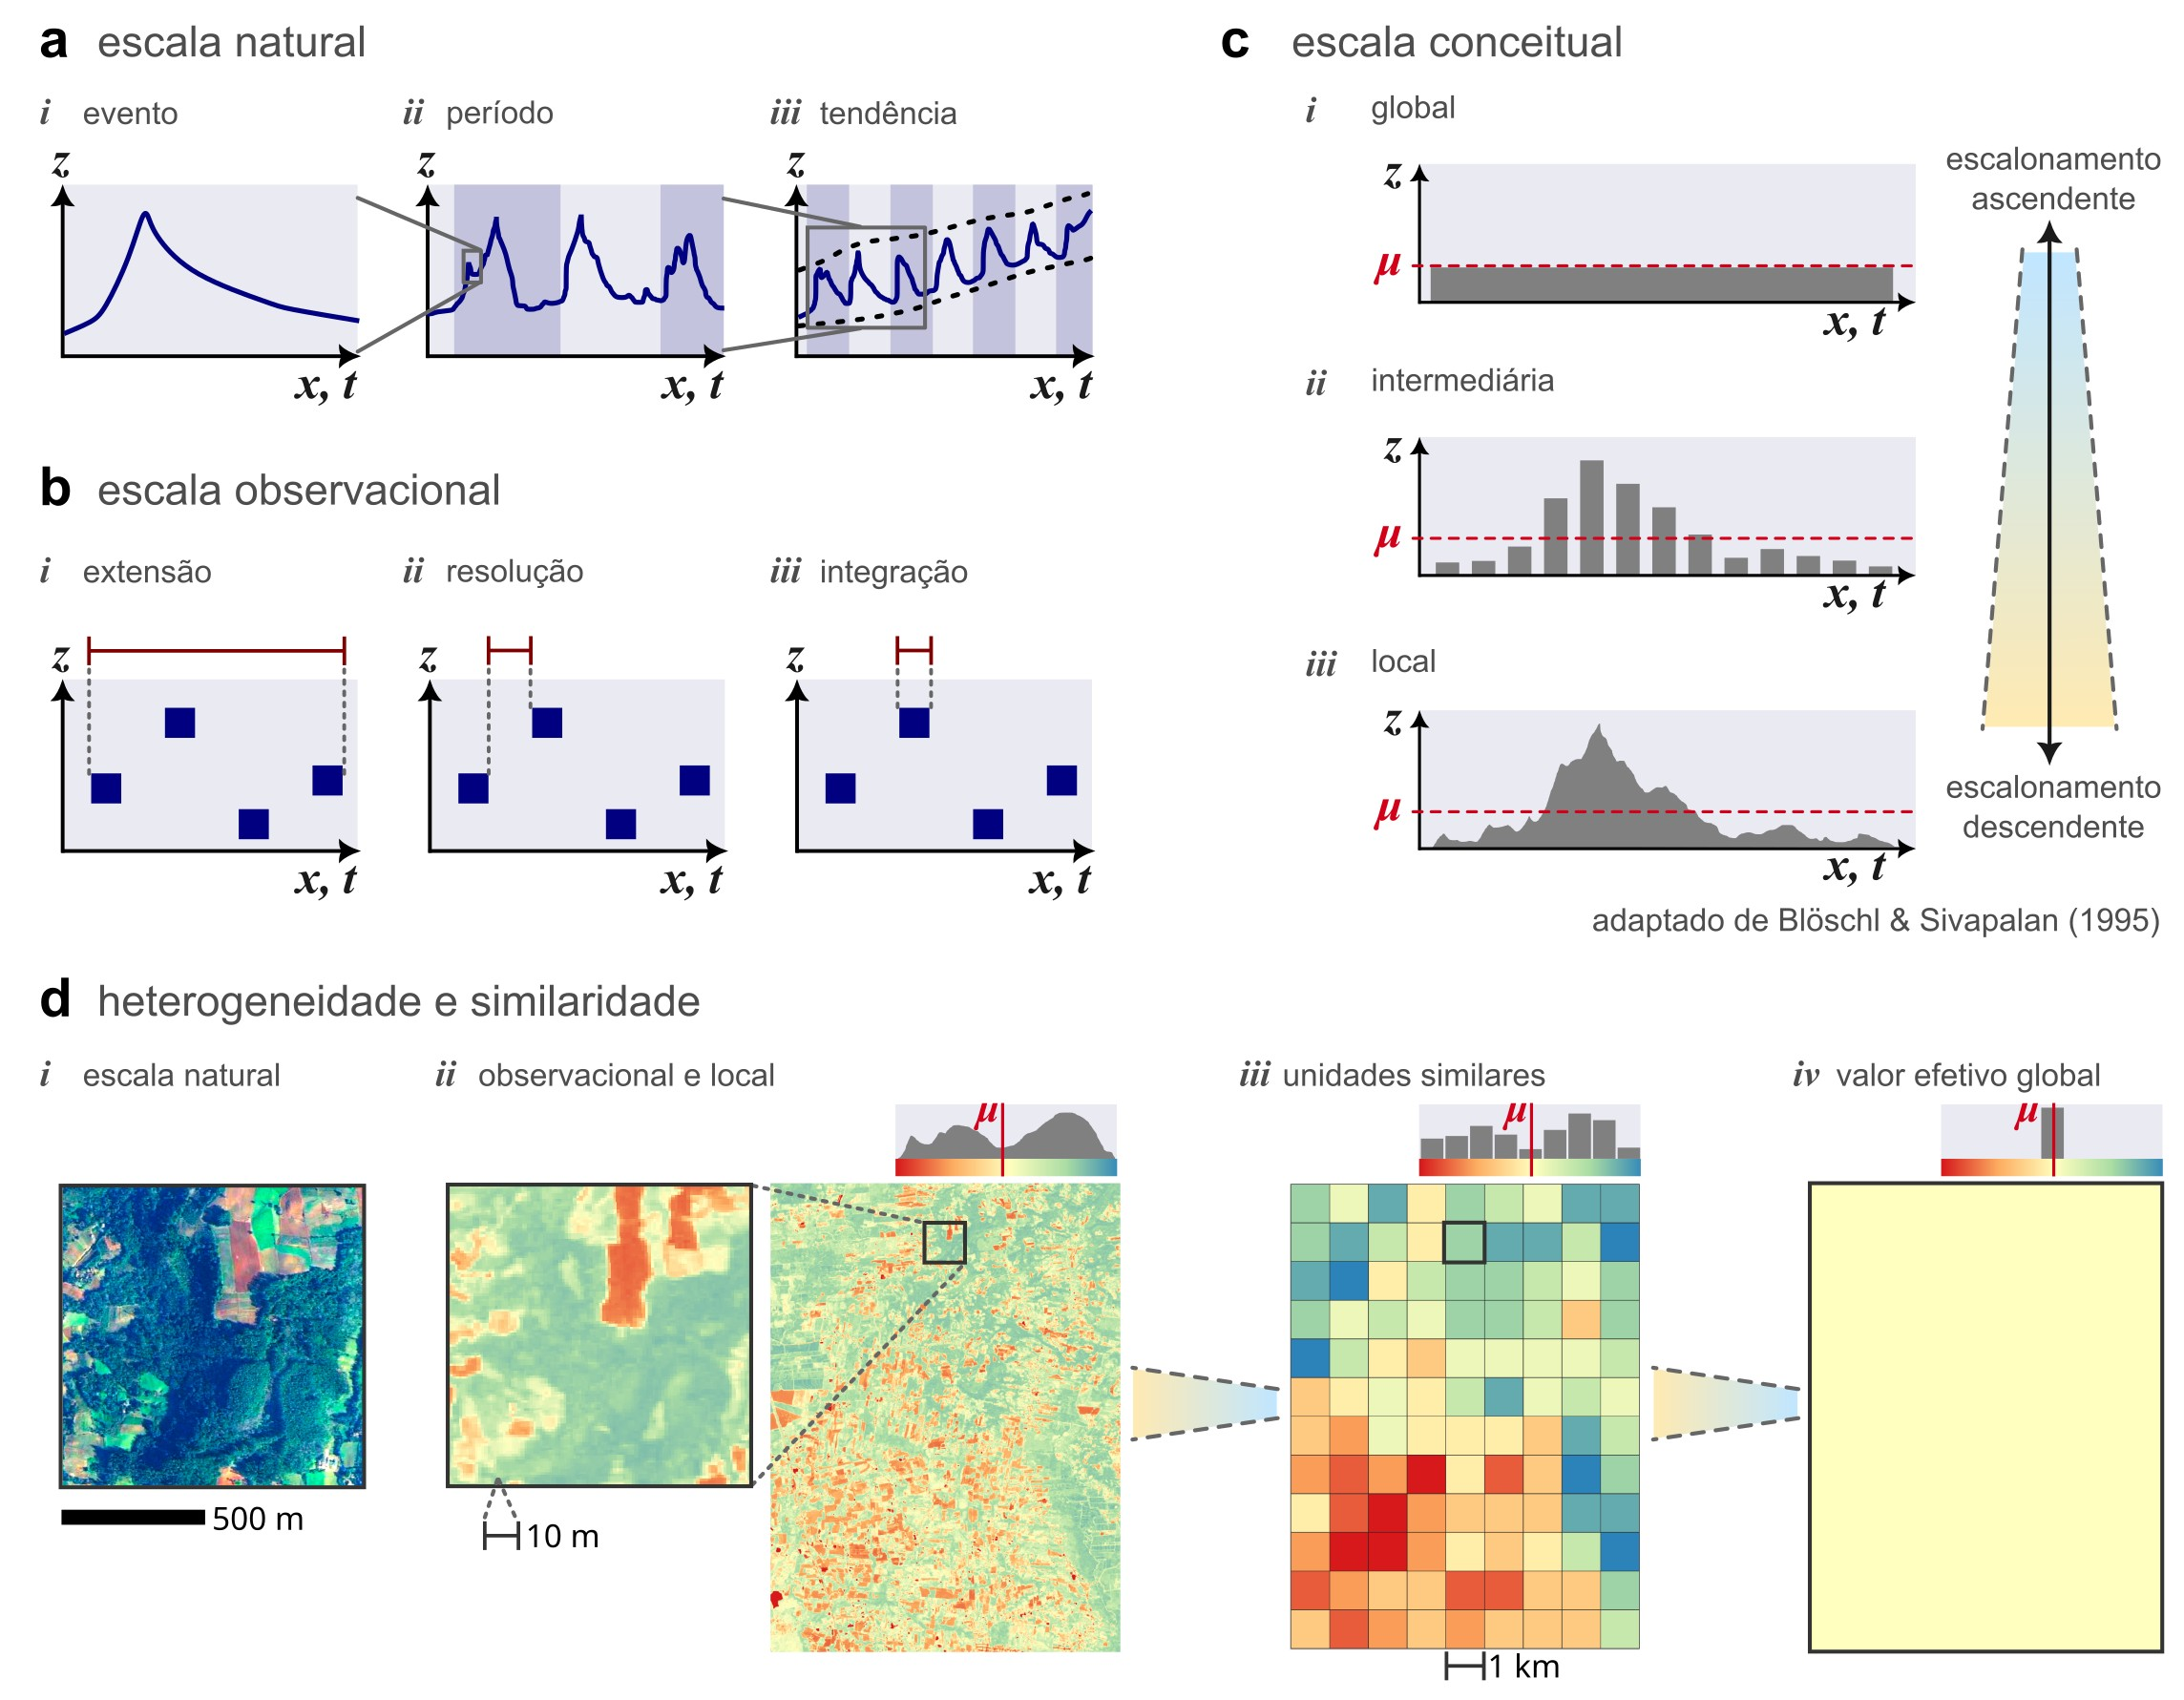
\includegraphics[width=0.98\linewidth]{figs/fig_scale.jpg}		
\caption[Sistematização das diferentes escalas]
{\textbf{---\;Sistematização das diferentes escalas.}
    Sistema organizado Blöschl \& Sivapalan (1995) \cite{Bloschl1995a} sobre as escalas a serem compatibilizadas no tempo e no espaço.\;\textbf{a}\;---\;A \gls{nat-scale} dos processos varia em: (\textrm{\textit{i}}) escala do evento; (\textrm{\textit{ii}}) escala do período, e; (\textrm{\textit{ii}}) escala da tendência.\;\textbf{b}\;---\;A \gls{obs-scale} apresenta três aspectos: (\textrm{\textit{i}}) extensão; (\textrm{\textit{ii}}) resolução, e; (\textrm{\textit{ii}}) integração.
    \;\textbf{c}\;---\;A \gls{model-scale} faz a mediação entre a \gls{nat-scale} e observacional pelos métodos de \gls{scalab}. O \gls{model} opera em escala aninhadas: (\textrm{\textit{i}}) \gls{glob-scale}; (\textrm{\textit{ii}}) escalas intermediárias, e; (\textrm{\textit{ii}}) \gls{loc-scale}.
    \;\textbf{d}\;---\;Valores efetivos através das escalas: \gls{nat-scale}, onde os processo ocorrem (\textrm{\textit{i}}); a \gls{obs-scale} estabelece o limite inferior da \gls{model-scale} local (\textrm{\textit{ii}}); escala intermediária de unidades similares (\textrm{\textit{iii}}), e; valor efetivo do processo na \gls{glob-scale} (\textrm{\textit{iv}}).
    
}
\label{fig:hydro:scaling} 		
\end{figure}


\par Blöschl \& Sivapalan (1995) também avançam para estabelecer a noção crucial de que existem três escalas a serem compreendidas e compatibilizadas em um exercício de modelagem: a \textbf{\gls{nat-scale}}, a \textbf{\gls{obs-scale}} e a \textbf{\gls{model-scale}} (Figura \ref{fig:hydro:scaling}). A \gls{nat-scale} refere-se à velocidade característica real exibida pelos processos hidrológicos. Ela pode ser classificada de diferentes maneiras: como o tempo de vida de \textbf{eventos} intermitentes, como enchentes; pelo \textbf{período} de eventos anuais, como o derretimento de neve ou a chegada de estações úmidas; ou pela duração das \textbf{tendências} em processos estocásticos de longa duração, que apresentam algum grau de autocorrelação, como a depleção ou o enchimento de aquíferos (Figura \ref{fig:hydro:scaling}\textbf{a}). Os autores também expandem essa ideia para escalas espaciais, definidas pela extensão e tendências no espaço, dependendo da natureza do processo. Alguns processos, como a precipitação, não têm uma escala preferencial, pois se distribuem em múltiplas escalas devido ao aninhamento de subprocessos de pequena e larga escala, geralmente com \textbf{lacunas espectrais} entre eles, ou seja, intervalos onde certas escalas são menos frequentes. O escoamento dos rios também segue essa estrutura de processos aninhados, com picos de enchentes resultantes de mecanismos de resposta rápida sobrepostos a mecanismos de resposta lenta, como o da água subterrânea ou a ocupação de grandes planícies de inundação. Mesmo as respostas rápidas ocorrem em diferentes escalas aninhadas, como enxurradas a partir de pequenas parcelas de solo e a formação de \gls{sat_areas} ou \gls{nasc_efemeras}, manifestando-se na escala da encosta. A \gls{obs-scale}, por sua vez, consiste na escala ocupada pelas evidências empíricas, surgindo da necessidade de se gerenciar um número finito de amostras. Ela possui três aspectos principais: a \textbf{extensão} ou cobertura do conjunto de dados, a \textbf{resolução} ou espaçamento entre as amostras, e o intervalo de \textbf{integração} da amostra (Figura \ref{fig:hydro:scaling}\textbf{b}). Se a amostragem fosse infinita (ou infinitesimal), a \gls{obs-scale} coincidiria com a \gls{nat-scale}, capturando até mesmo o ruído amostral. Já uma amostragem muito esparsa captura apenas a tendência do processo, na melhor das hipóteses. Um exemplo típico disso é um pluviômetro que, ao ser lido diariamente, reporta a chuva acumulada em um intervalo de um dia, intervalo esse que pode ser muito maior que a duração natural de uma chuva que ocorreu por apenas alguns minutos. Ainda assim, essa leitura captura a tendência das chuvas em uma escala semanal ou mensal. Por outro lado, amostras detalhadas de solo podem fornecer informações sobre a condutividade hidráulica extremamente localizada, que não refletem o efeito real de macroporos e caminhos preferenciais na escala da encosta. Nesse caso, a escala do processo é mais ampla, tornando as amostras pontuais incomensuráveis. Idealmente, as observações devem ser compatíveis com a escala dos processos de interesse, posicionando a amostragem em um ponto ótimo entre a faixa de ruído e a faixa de tendência. 

\par A \gls{nat-scale} e a \gls{obs-scale} relacionam-se na modelagem hidrológica ao serem mediadas pela \gls{model-scale}, que é a escala de representação do \gls{model} em si (Figura \ref{fig:hydro:scaling}\textbf{c}). É aqui que reside o desafio da \gls{scalab}, pois geralmente a \gls{model-scale} é muito maior ou muito menor que a \gls{obs-scale}, o que introduz o inevitável \gls{error-commensu} $\varepsilon_{\Delta}$. Como discutido anteriormente, tanto o reservatório de solo instanciado pela \gls{sys-dyn} quanto um elemento de \gls{comp-grid} em um \gls{model} fisicamente embasado representam blocos maciços que são incomensuráveis com qualquer observação pontual obtida em campo. Ainda assim, esse erro pode ser minimizado ao se representar o \gls{sys-target} simultaneamente em escalas aproximadas às observações disponíveis. Na prática, isso significa dividir o \gls{model} em pelo menos dois patamares aninhados: uma \textbf{\gls{glob-scale}}, mais agregada, e uma \textbf{ \gls{loc-scale}}, mais detalhada. Escalas intermediárias também podem ser incrementalmente instanciadas, dependendo dos processos hidrológicos simulados e das observações disponíveis. Na \gls{glob-scale}, por exemplo, são representados os processos altamente agregados da bacia hidrográfica, como o escoamento fluvial em uma seção do rio e o fluxo final de evapotranspiração, resultados acumulados de diversos subprocessos em escalas menores. Já na \gls{loc-scale}, são representados os detalhes desses subprocessos em pequenas parcelas ou elementos de malha, como a entrada de chuva e a geração de escoamento em diferentes partes da paisagem. Nesse sentido, as variáveis de armazenamento e de fluxo, os \gls{parameters} e os \gls{input-data} precisam ser compatibilizados em todos os níveis, sendo necessário transferir informação de um nível para outro, ou seja, precisam ser escalonados. 

\par A saída para essa situação, portanto, consiste na definição de uma \textbf{\gls{scaling-func}} que seja válida entre os patamares simulados. Essas funções realizam tanto o \textbf{\gls{upscaling}}\footnote{Tradução de \textit{upscaling}, no inglês.} da informação (transferência de baixo para cima) quanto o \textbf{\gls{downscaling}}\footnote{Tradução de \textit{downscaling}, no inglês.} da informação (transferência de cima para baixo). Para níveis e fluxos materiais, que se conservam, a função de \gls{upscaling} pode ser simplesmente a média ou a soma em uma dada extensão espacial ou temporal. O fluxo de evapotranspiração global de uma bacia hidrográfica, assim, seria a média dos fluxos locais (a integral). O \gls{downscaling}, por outro lado, geralmente consiste em um processo não trivial que depende fortemente do processo em questão. No caso das propriedades dos solos e das rochas, como a condutividade hidráulica, a única forma de descompactar essa informação é a partir de mapas que revelem o seu padrão ou \textbf{\gls{hetspatial}}. A mesma estratégia de mapeamento se aplica para \gls{parameters} relacionados com a vegetação ou cobertura do solo, como a \gls{intercep-capacity} e a \gls{sfmax}. Na ausência de informações diretas, o uso de \textbf{co-variáveis} ou indicadores pode ser empregado com uma função de \gls{downscaling}, ou \textbf{\gls{downscaling2}}, o que adiciona novas \gls{aux-hyp} ao arcabouço teórico do \gls{model}. Por exemplo Collischonn et \textit{al.} (2007) \cite{Collischonn2007} assumem a \gls{hipotese} de que a \gls{intercep-capacity} local é diretamente proporcional ao Índice de Área Foliar (LAI), ou seja: $c_{\text{max}, i} = c \cdot \texttt{LAI}_{i}$, em que $c$ é uma constante de proporcionalidade. Por outro lado, as co-variáveis podem ser aplicadas para \textit{agrupar} regiões espaciais que exibem, teoricamente, \textbf{\gls{hydro-simi}}, ou seja, são regiões suficientemente homogêneas em relação um determinado processo na escala avaliada. Nesse contexto, a co-variável denomina-se \textbf{índice de similaridade hidrológica}. As regiões homogêneas resultantes desse agrupamento, denominadas de \textbf{\gls{urh}}, reduzem sobremaneira o custo computacional já que executam um processamento em blocos, em oposição ao processamento em malha requerido na \gls{loc-scale}. Assim, os modelos que aplicam essa abordagem no \gls{downscaling} são tidos como \textbf{\gls{models-semid}}, pois não representam a \gls{loc-scale} de forma completamente explícita, a informação ainda está compactada em na escala intermediária das \gls{urh}. Por fim, outro desafio na \gls{loc-scale} consiste na \textbf{\gls{regionalization}} de valores localizados em pontos ou manchas para suas vizinhanças laterais, na mesma escala, como no caso de observações de chuva pontuais que são interpoladas para representar um campo contínuo no espaço. Assim como no caso da \gls{downscaling2} de \gls{parameters}, esse processo de interpolação introduz novas \gls{aux-hyp} (e suas incertezas) no processo de modelagem.

\subsection{\texttt{TOPMODEL}} \label{sec:hydro:topmodel}

\par Um exemplo de \gls{scalab} que convém apresentar neste momento é o \gls{model} \texttt{TOPMODEL}, articulado inicialmente por Beven \& Kirkby (1979) em um estudo na bacia Crimple Beck (Inglaterra, 8 km²) \cite{Beven1979a}. Esse \gls{model}, instanciado no \gls{paradigma} da \gls{sys-dyn}, apesar de exibir uma estrutura de compartimentos relativamente simples, representa de forma eficaz o mecanismo da \gls{vsa}, produzindo respostas hidrológicas rápidas tanto por enxurradas quanto pelo excesso de saturação nas áreas úmidas. Durante a simulação, o \gls{model} representa explicitamente a expansão e retração das \gls{sat_areas} ao longo do talvegue do terreno, conforme a bacia hidrográfica recebe mais ou menos chuva. O fluxo de \gls{ground-rain} que incide diretamente sobre as áreas saturadas torna-se eventualmente parte da resposta rápida de eventos de enchente, enquanto a porção restante da \gls{ground-rain} incide sobre o solo seco, podendo então se infiltrar. 

% figure
\begin{figure}[t!] 
\centering				
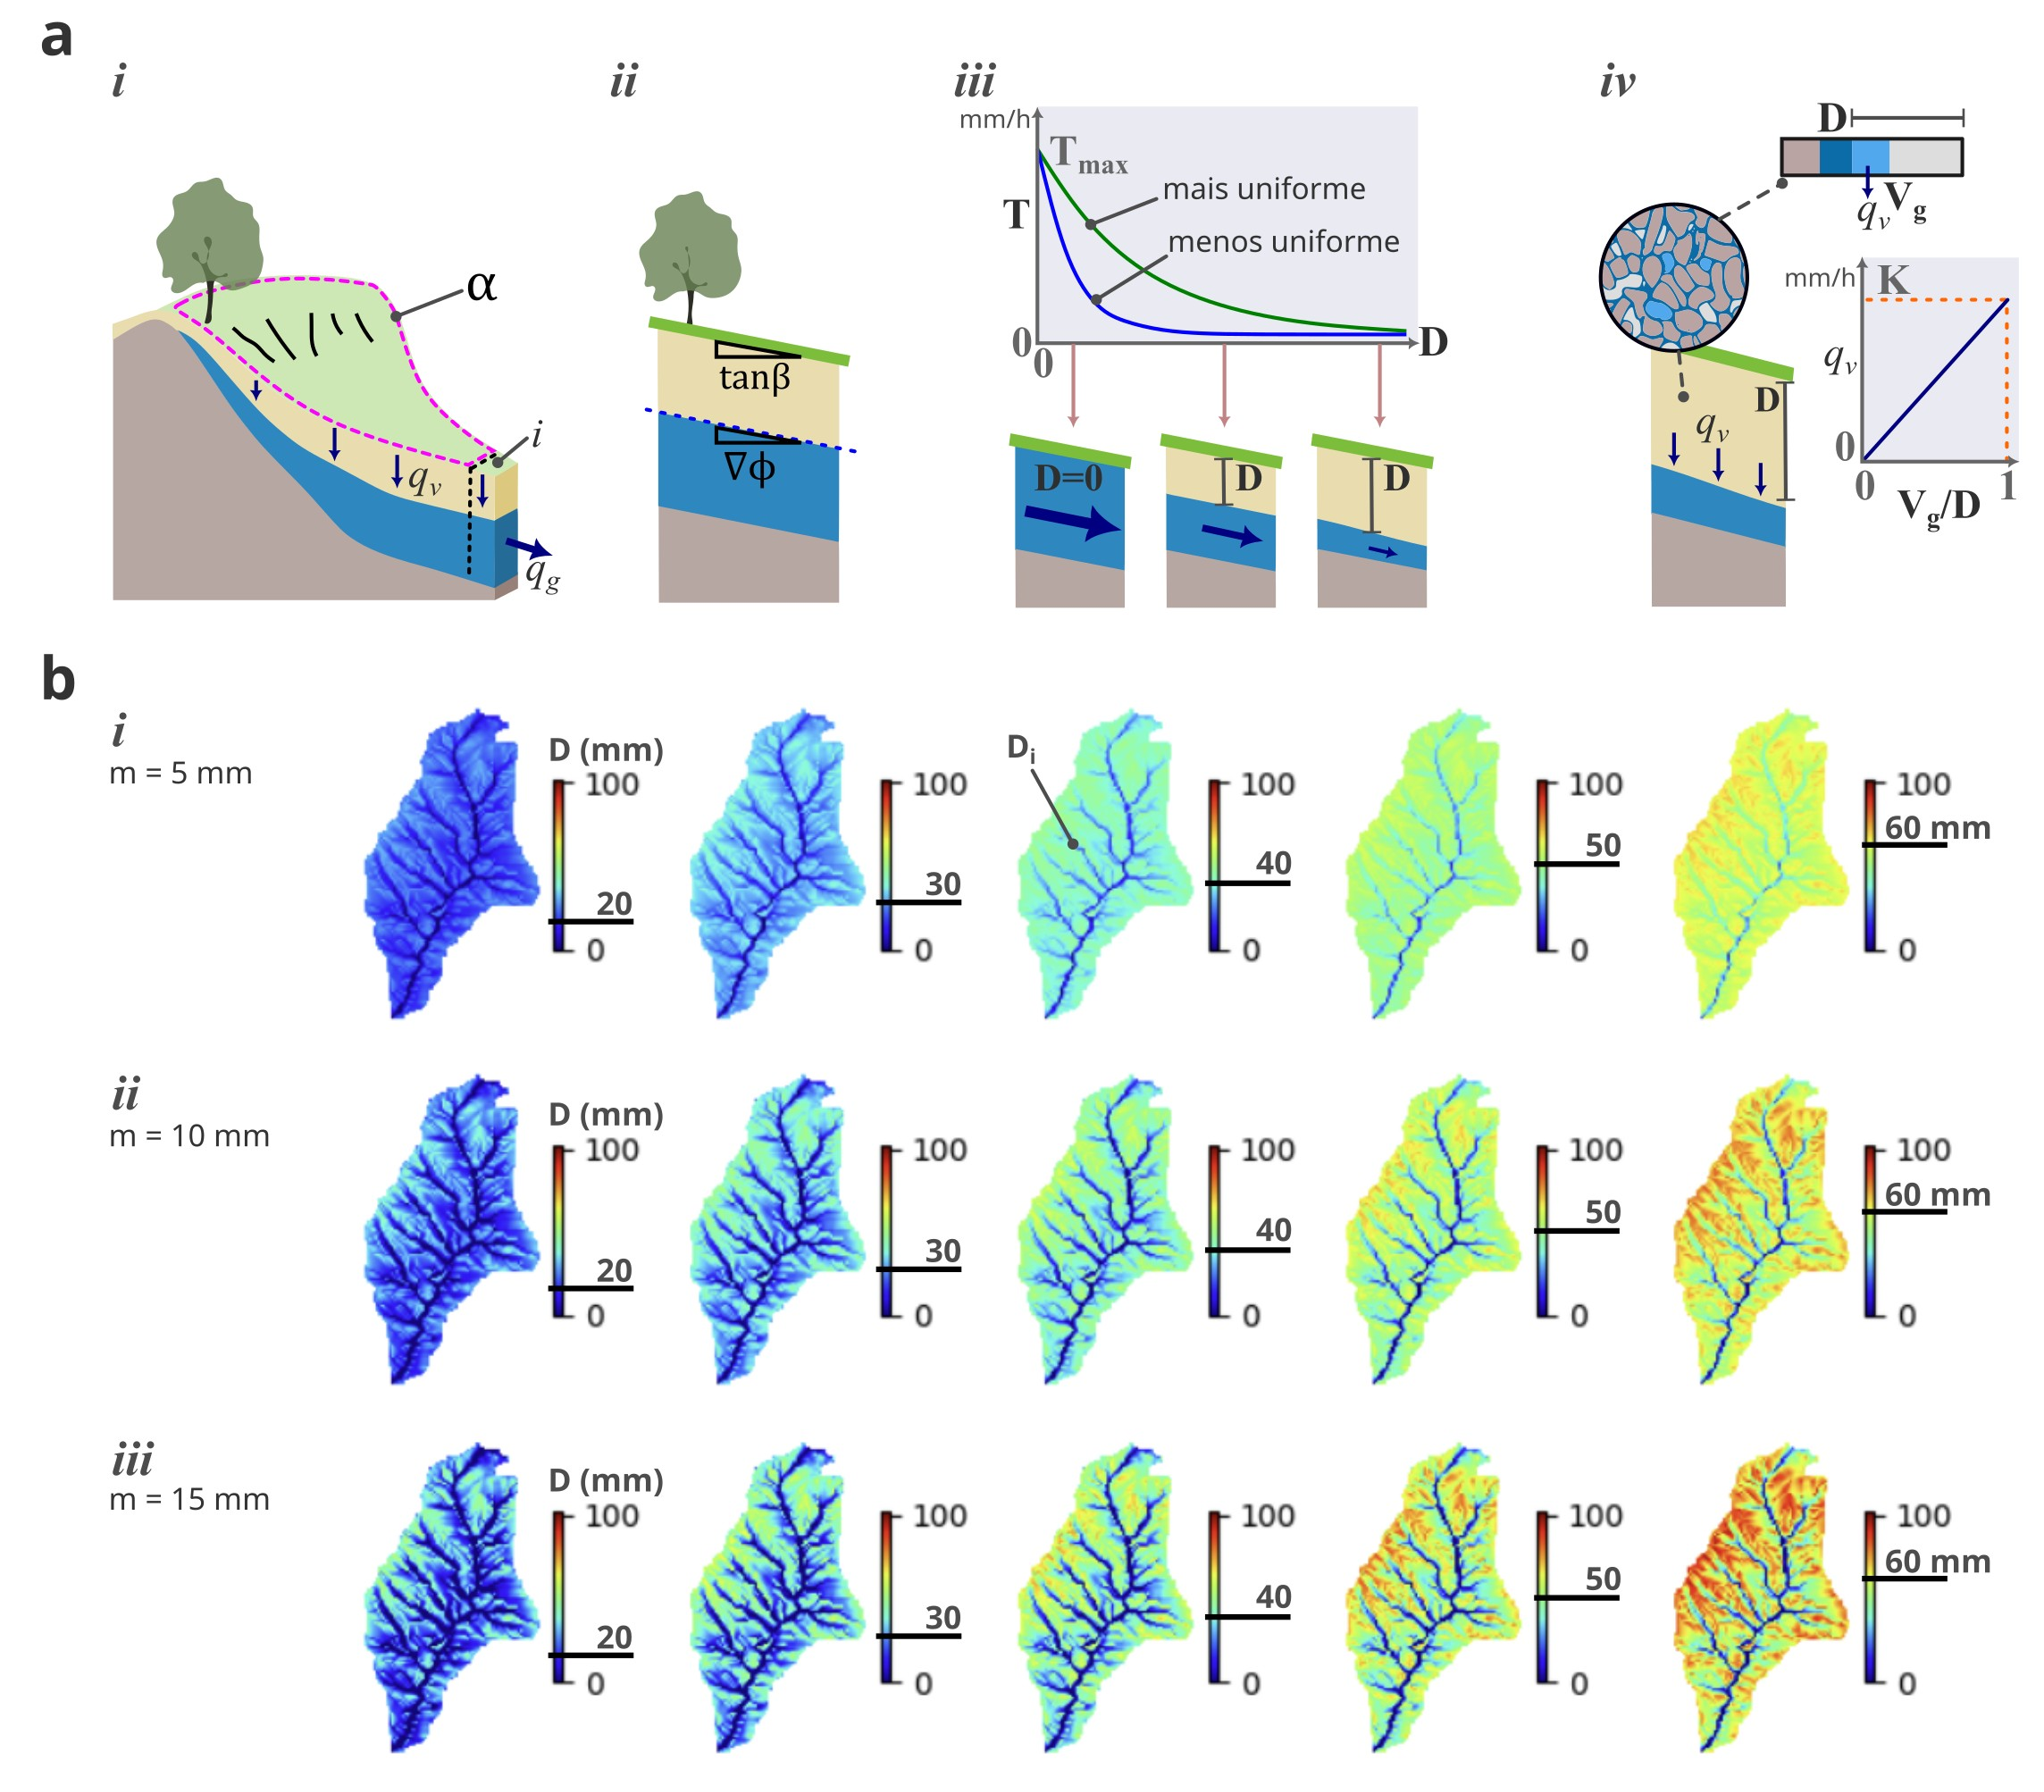
\includegraphics[width=0.98\linewidth]{figs/fig_topmodel.jpg}		
\caption[Hipóteses e implicações do \texttt{TOPMODEL}]
{\textbf{---\;Hipóteses e implicações do \texttt{TOPMODEL}.}
    O \texttt{TOPMODEL} é um \gls{model} que realiza o \gls{downscaling} da saturação no solo a partir de um índice topográfico de saturação, o \gls{twi}.\;\textbf{a}\;---\;O \texttt{TWI} na versão clássica do \gls{model} é obtido ao se aplicar a \gls{darcy-law} com três \gls{aux-hyp}: a \gls{hipotese} de estado estacionários (detalhe \textrm{\textit{i}}); a \gls{hipotese} de solos rasos (detalhe \textrm{\textit{ii}}), e; a \gls{hipotese} de decaimento vertical da transmissividade (detalhe \textrm{\textit{iii}}). Uma quarta \gls{hipotese} auxiliar é o fluxo de \gls{qv} como uma função linear da pressurização da \gls{unsat-zone} (detalhe \textrm{\textit{iv}}).\;\textbf{b}\;---\;A aplicação da \gls{scaling-func} do \gls{model} utiliza o distribui o \texttt{TWI} (detalhe \textrm{\textit{i}}) para se determinar o \gls{dgrav} e as \gls{sat_areas} na escala na \gls{loc-scale} (detalhe \textrm{\textit{ii}} e \textrm{\textit{iii}}).\;\textbf{c}\;---\; Os detalhes \textrm{\textit{i}} e \textrm{\textit{ii}} comparam a sensibilidade da distribuição local do déficit para solos mais ou menos uniformes (parâmetro $m$). Uma bacia com solo mais uniforme ($m$ alto) exibe uma distribuição de déficits mais dispersa do que uma bacia com solo menos uniforme ($m$ baixo). 
}
\label{fig:hydro:topmodel} 		
\end{figure}


\par Ao contrário do alto custo computacional dos \gls{models-phys}, que precisam resolver numericamente a Equação de Darcy-Richards em uma \gls{comp-grid}, a abordagem do \texttt{TOPMODEL} identifica o padrão espacial de saturação do solo na \gls{loc-scale} por meio de uma função de \gls{downscaling} (distribuição) de baixo custo computacional. Diante de evidências empíricas apenas de chuva e vazão, as duas abordagens são empiricamente equivalentes, com a vantagem de que o \texttt{TOPMODEL} é mais simples (ou seja, possuiu um maior grau de falseabilidade). Nesse sentido, o uso de um \gls{model} fisicamente embasado passa a ser justificado somente quando evidências mais detalhadas se tornam disponíveis, tais como níveis piezométricos, \gls{bedrock_topo} e \gls{parameters} de qualidade da água\footnote{Para mapeamentos detalhados da evolução de plumas de contaminação no subsolo, por exemplo, um \gls{model} fisicamente embasado consiste na única alternativa que oference a ontologia compatível com o problema em questão.}.

\par A saturação do solo no \texttt{TOPMODEL} é expressa pelo \gls{dgrav} na \gls{loc-scale} na bacia hidrográfica, denotado por $D_{i} \; [\text{L}]$, onde $i$ é um elemento qualquer de uma malha que divide a bacia em $N$ elementos. Ou seja, quando $D_{i} = 0$, o solo está completamente saturado no elemento $i$ e a água da \gls{ground-rain} incidente sobre esse elemento não poderá se infiltrar, restando acumular-se na superfície até atingir a \gls{sfmax}. A função de compactação dessa variável transfere a informação através das escalas pelo simples cálculo da média:
\begin{linenomath*}
\begin{equation}
\label{eq:topmodel:d1}
D = \frac{1}{N} \sum^{N}_{i} D_{i} \quad  \forall \; i \in \{ 1, 2, ..., N\}
\end{equation}
\end{linenomath*}
Em que $D \; [\text{L}]$ é o déficit global e; $D_{i} \; [\text{L}]$ é o déficit local. Ou seja, o \gls{dgrav} na \gls{glob-scale} consiste na média dos déficits na \gls{loc-scale} $D_{i}$. A distribuição do déficit gravitacional da \gls{glob-scale} para a \gls{loc-scale}, por outro lado, fundamenta-se no uso de um \textbf{\gls{tsi}}. Esse índice, assim, é tido como uma \textit{co-variável} do déficit gravitacional, de forma que os \textit{desvios da média} entre a \gls{loc-scale} e global são linearmente proporcionais:
\begin{linenomath*}
\begin{equation}
\label{eq:topmodel:d2}
D - D_{i}  \propto \lambda_{i} - \lambda  \quad \forall \; i
\end{equation}
\end{linenomath*}
Em que $\lambda_{i}\; [-]$ é o \gls{tsi} na \gls{loc-scale}, e; $\lambda \; [-]$ é o \gls{tsi} na \gls{glob-scale}, ou seja, a média obtida por:
\begin{linenomath*}
\begin{equation}
\label{eq:topmodel:d3}
\lambda = \frac{1}{N} \sum^{N}_{i} \lambda_{i} \quad  \forall \; i 
\end{equation}
\end{linenomath*}
A Equação \eqref{eq:topmodel:d2} torna-se em uma igualdade ao se introduzir uma constante de proporcionalidade:
\begin{linenomath*}
\begin{equation}
\label{eq:topmodel:d4}
D - D_{i}  = \omega (\lambda_{i} - \lambda ) \quad \forall \; i
\end{equation}
\end{linenomath*}
Em que $\omega \; [\text{L}]$ é o fator de \gls{scalab}. Com o remanejo dos termos, o déficit gravitacional local $D_{i}$ é obtido pela seguinte \gls{downscaling2}:
\begin{linenomath*}
\begin{equation}
\label{eq:topmodel:d5}
D_{i}  = D + \omega (\lambda - \lambda_{i}) \quad \forall \; i
\end{equation}
\end{linenomath*}
Em que $D_i$ deve ser truncado em zero, de maneira a não assumir valores negativos. Em um \gls{model} hidrológico, a Equação \eqref{eq:topmodel:d5} objetiva distribuir localmente o déficit global $D$ a cada passo de tempo, permitindo que outras variáveis na \gls{loc-scale} possam ser especificadas, como a \gls{qv} e o escoamento superficial. Nesse caso, os elementos $i$ onde $D_i = 0$ correspondem precisamente nas áreas de solo saturado, a \gls{vsa} que invariavelmente irá produzir respostas rápidas de escoamento diante de eventos de chuva. 

\par Aqui, cabe destacar que a Equação \eqref{eq:topmodel:d5} é uma formulação genericamente aplicável para qualquer \gls{tsi} $\lambda_{i}$. Contudo, originalmente Beven \& Kirkby (1979) a deduziram teoricamente a partir da \gls{darcy-law} e algumas \gls{aux-hyp} (ver Figura \ref{fig:hydro:topmodel}\textbf{a}), o que resultou no \gls{tsi} $\lambda_{i}$ então denominado \textbf{\gls{twi}}, que é calculado por:
\begin{linenomath*}
\begin{equation}
\label{eq:topmodel:twi}
\text{T}_{i}  = \ln{(\alpha_{i}/\tan \beta_{i})} \quad \forall \; i
\end{equation}
\end{linenomath*}
Em que $\alpha_{i}\; [L^{2}L^{-1}]$ é a área de drenagem local por unidade de contorno, e;  $\beta_{i} [-]$ é a declividade local do terreno. Ou seja: o potencial local de saturação do solo (1)  é maior quanto maior a área de drenagem, e (2) é maior quanto menor for a declividade do terreno. Mapas de \acrshort{atwi} podem assim ser obtidos diretamente de um \textbf{\gls{dem}} com a aplicação de técnicas de geoprocessamento. A declividade local $\beta_{i}$, por exemplo, pode ser estimada pelo método de Horn (1981) \cite{Horn1981a} ao se computar as diferenças de altitude oeste-leste e norte-sul na \textbf{mantissa}\footnote{Em uma malha retangular de elementos, a mantissa consiste nos oito elementos vizinhos no entorno de um elemento qualquer.} do elemento de malha. A determinação da área de drenagem local por unidade de contorno $\alpha_{i}$, por outro lado, consiste em uma análise mais intensiva em termos computacionais, pois é necessário rastrear todos os elementos de malha à montante de cada elemento qualquer. Isso não pode ocorrer antes se remover depressões espúrias no \acrshort{adem}, que fazem o método truncar. Barnes et \textit{al.} (2014) \cite{Barnes2014a} introduzem um algoritmo eficiente para esse processo, assim como revisam diversas outras estratégias disponíveis na literatura. Uma vez obtido um \acrshort{adem} sem depressões, a área de drenagem é computada por métodos de acúmulo de fluxo, como o método de fluxo unidirecional de O'Callaghan \& Mark (1984) \cite{Ocallaghan1984a} ou o método de fluxo multidirecional de Freeman (1991) \cite{Freeman1991a}. Quinn et \textit{al.} (1991) \cite{Quinn1991b} demonstram que há uma sensibilidade substantiva no \texttt{TOPMODEL} diante da escolha do método de acúmulo de fluxo, sugerindo que o método multidirecional apresenta melhor adequação empírica. Além disso, os autores também avaliam a possibilidade de \textit{sobreposição} de métodos, para ajustar o \acrshort{atwi} entre a regiões de drenagem efêmera (multidirecional) e perene (unidirecional).

\par São três \gls{aux-hyp} que fundamentam teoricamente a Equação \eqref{eq:topmodel:twi}. A primeira delas é a \gls{hipotese} de estado estacionário (detalhe \textit{i} na Figura \ref{fig:hydro:topmodel}\textbf{a}), a noção que se estabelece uma condição local de estado estacionário a cada passo de tempo, de maneira que o escoamento de base lateral é igual ao fluxo de recarga:
\begin{linenomath*}
\begin{equation}
\label{eq:topmodel:prem1}
q_{\text{g}, i} = q_{\text{v}} \cdot \alpha_{i}  \quad \, \forall i
\end{equation}
\end{linenomath*}
Em que $q_{\text{g}, i}\; [L^{2}T^{-1}]$ é o fluxo de base lateral por unidade de contorno; $q_{\text{v}}\; [LT^{-1}]$ é o fluxo de recarga, e; $\alpha_{i}\; [L^{2}L^{-1}]$ é a área de drenagem local por unidade de contorno. A segunda \gls{hipotese} auxiliar (detalhe \textit{ii} na Figura \ref{fig:hydro:topmodel}\textbf{a}) assume que o solo é raso o suficiente para que o gradiente hidráulico local na zona freática $\nabla \Phi_{i}\; [LL^{-1}]$ seja aproximado pela declividade local do terreno $\tan \beta_{i}\; [LL^{-1}]$:
\begin{linenomath*}
\begin{equation}
\label{eq:topmodel:prem2}
\nabla \Phi_{i} = \tan \beta_{i} \quad \, \forall i
\end{equation}
\end{linenomath*}
A terceira \gls{hipotese} auxiliar (detalhe \textit{ii} na Figura \ref{fig:hydro:topmodel}\textbf{a}) é que condutividade hidráulica local $K_{ i}\; [LT^{-1}]$ decai exponencialmente com o déficit gravitacional, ou seja, quanto mais seco o solo, menor é condutividade hidráulica. Essa é uma \gls{hipotese} coerente com as observações empíricas de que os horizontes superiores do solo, com camadas orgânicas e macroporos, exibem uma condutividade maior que as partes inferiores, mais minerais. A condutividade hidráulica por unidade de contorno é expressa como a \textbf{\gls{trans-hyd}}, de fazendo a \gls{hipotese} assumir a seguinte forma: 
\begin{linenomath*}
\begin{equation}
\label{eq:topmodel:prem3}
\kappa_{i} = \kappa_{\text{max}} \cdot e^{-D_{i}/m}  \quad \, \forall i
\end{equation}
\end{linenomath*}
Em que $\kappa_{i}\; [L^{2}T^{-1}]$ é a transmissividade local; $\kappa_{\text{max}}\; [L^{2}T^{-1}]$ é a transmissividade máxima em condições saturadas; $D_{i}\; [L]$ é o déficit local, e; $m\; [L]$ é a constante de \textbf{uniformidade vertical do solo}. Quanto maior o valor de $m$, mais gradual é a mudança da transmissividade em função da saturação, de maneira que: $\lim_{m\to\infty} T = T_{\text{max}}$. Ao se considerar os fluxos por unidade de contorno do terreno, a Equação de Darcy \eqref{eq:darcy-5} assume a seguinte estrutura:
\begin{linenomath*}
\begin{equation}
\label{eq:topmodel:darcy1}
u = K \nabla \Phi \Rightarrow q_{\text{g,i}} = \kappa_{\text{max}} \nabla \Phi_{i} \quad \, \forall i
\end{equation}
\end{linenomath*}
Em que a velocidade darciana $u \; [LT^{-1}]$ corresponde ao escoamento de base lateral por unidade de contorno $q_{\text{g}, i}\; [L^{2}T^{-1}]$. Conectando as Equações \eqref{eq:topmodel:prem1}, \eqref{eq:topmodel:prem2} e \eqref{eq:topmodel:prem3} na Equação de Darcy \eqref{eq:topmodel:darcy1}:
\begin{linenomath*}
\begin{equation}
\label{eq:topmodel:darcy2}
q_{\text{v}} \alpha_{i} = \kappa_{\text{max}} e^{-D_{i}/m} \tan \beta  \quad \, \forall i
\end{equation}
\end{linenomath*}
O déficit local $D_i$ pode ser isolado, de forma que:
\begin{linenomath*}
\begin{equation}
\label{eq:topmodel:darcy3}
D_{i} = -m \ln{(q_{\text{v}} \alpha_{i} /\kappa_{\text{max}}\tan \beta_{i})}  \quad \, \forall i
\end{equation}
\end{linenomath*}
Pelas propriedades logarítmicas, também chega-se na seguinte relação, que isola os termos das variáveis hidrológicas  estáticas, das variáveis hidrológicas dinâmicas e os termos puramente topográficos :
\begin{linenomath*}
\begin{equation}
\label{eq:topmodel:plug1}
\ln(q_{\text{v}}/\kappa_{\text{max}}) = - D_{i}/m - \ln(\alpha_{i} / \tan \beta_{i})  \quad \, \forall i
\end{equation}
\end{linenomath*}
Agora, considerando que o déficit global $D$ é a média dos déficits locais $D_i$, a Equação \eqref{eq:topmodel:darcy3} pode ser aplicada na Equação \eqref{eq:topmodel:d1}:
\begin{linenomath*}
\begin{equation}
\label{eq:topmodel:d6}
D = \frac{1}{N} \sum^{N}_{i} -m \ln{(q_{\text{v}} \alpha_{i} /\kappa_{\text{max}}\tan \beta_{i})} \quad  \forall \; i 
\end{equation}
\end{linenomath*}
Pelas propriedades dos somatórios e assumindo $m$ e $\kappa_{\text{max}}$ espacialmente homogêneos, os termos locais podem ser isolados dos termos globais:
\begin{linenomath*}
\begin{equation}
\label{eq:topmodel:d7}
D = \left[ -m\frac{1}{N} \sum^{N}_{i} \ln{(\alpha_{i}/\tan \beta_{i})}\right]  - \left[m \ln{(q_{\text{v}} /\kappa_{\text{max}})}\right] \quad  \forall \; i 
\end{equation}
\end{linenomath*}
Substituindo \eqref{eq:topmodel:plug1} em \eqref{eq:topmodel:d7}, chega-se em:
\begin{linenomath*}
\begin{equation}
\label{eq:topmodel:d8}
D = \left[ -m\frac{1}{N} \sum^{N}_{i} \ln{(\alpha_{i}/\tan \beta_{i})}\right] + D_{i} + m \ln{(\alpha_{i}/\tan \beta_{i})} \quad  \forall \; i 
\end{equation}
\end{linenomath*}
Que é homóloga à Equação \eqref{eq:topmodel:d4}, sendo $\lambda_{i} = \text{T}_{i} $ e $\omega = m$:
\begin{linenomath*}
\begin{equation}
\label{eq:topmodel:d9}
D_{i}= D +   m  \left[ \left( \frac{1}{N} \sum^{N}_{i} \text{T}_{i}\right) - \text{T}_{i}\right] \quad  \forall \; i 
\end{equation}
\end{linenomath*}

\par No total, a versão do \texttt{TOPMODEL} articulada em Beven \& Kirkby (1979) apresenta sete \gls{parameters} regulando reservatórios e fluxos do balanço hídrico no solo, assim como um parâmetro de velocidade de escoamento, empregado na simulação da propagação de vazão na rede de drenagem de canais. Em especial, os \gls{parameters} $m$ e $Q_{\text{g},\text{max}}$ podem ser estimados \textit{a priori} a partir da \gls{deple-curve} do rio durante estiagens observadas em tempo frio (com baixas perdas de água por evapotranspiração), uma vez que a integração da Equação \eqref{eq:topmodel:prem3} por todos os trechos laterais de canais determina o escoamento de base:
\begin{linenomath*}
\begin{equation}
\label{eq:topmodel:prem3a}
Q_{\text{g}, t} = Q_{\text{g},\text{max}} \cdot e^{-D_{t}/m}  \quad \forall \; t
\end{equation}
\end{linenomath*}
Em que $Q_{\text{g}}\;[L^{3}T^{-1}]$ é o escoamento de base; $Q_{\text{g},\text{max}}\;[L^{3}T^{-1}]$ é a capacidade de produção do aquífero; $D_t\;[\text{L}]$ é o déficit global no tempo $t$, e; $m\; [L]$ é a uniformidade vertical do solo. Os detalhes na Figura \ref{fig:hydro:topmodel}\textbf{b} demonstram o quanto o \gls{model} é sensível diante de mudanças na uniformidade vertical do solo. A distribuição do déficit local, nessa linha, torna-se incrementalmente mais dispersa, à medida que o valor de $m$ aumenta. Isso ocorre evidentemente em razão desse ser um multiplicador na \gls{scaling-func} (Equação \eqref{eq:topmodel:d5}). A implicação prática é que uma bacia com solo relativamente mais uniforme irá produzir relativamente mais \gls{sat_areas}. A interpretação física dessa implicação é que, mantida a mesma capacidade de produção do aquífero $Q_{\text{g},\text{max}}$, um solo mais uniforme transmite mais água, drenando as encostas mais altas mais rapidamente à medida que o déficit global da bacia aumenta. 

\par A \gls{cond-hyd} do solo é empregada no \texttt{TOPMODEL} em uma revisão do \gls{model} apresentada por Beven \& Wood (1983) \cite{Beven1983a}, sob uma quarta \gls{aux-hyp} sobre o fluxo de \gls{qv} (detalhe \textit{iv} na Figura \ref{fig:hydro:topmodel}\textbf{a}). Nesse caso, os autores assumem que o fluxo vertical de \gls{qv} na \gls{loc-scale} tende linearmente para o valor da \gls{cond-hyd} à medida que a \gls{unsat-zone} torna-se pressurizada pela carga hidráulica\footnote{Na verdade, os autores introduziram um estranho termo de \say{atraso por unidade de déficit} $t_d\; [TL^{-1}]$, fazendo a equação da recarga assumir a seguinte forma: $q_v = V_g / t_d D$. Ainda que idêntica, essa notação não faz muito sentido hidrológico, principalmente considerando que a condutividade hidráulica é um conceito bem estabelecido. Em observâncias aos princípios de modelagem de John Sterman (Capítulo 2), mantive uma notação mais clara.}:
\begin{linenomath*}
\begin{equation}
\label{eq:topmodel:qv}
q_{\text{v}, i} = K \cdot \frac{V_{\text{g}, i}}{D_i}  \quad \forall \; i
\end{equation}
\end{linenomath*}
Em que $q_{\text{v}, i}\;[LT^{-1}]$ é a recarga local; $K\;[LT^{-1}]$ é a condutividade hidráulica do solo; $V_{\text{g}, i}\;[L]$ é a água gravitacional local na \gls{unsat-zone}, e; $D_{i} \; [\text{L}]$ é o déficit local. Ou seja, a pressurização na \gls{unsat-zone} é representada pela razão entre a água gravitacional e o déficit de saturação, que também pode ser interpretado como a \textit{capacidade} de armazenamento de água gravitacional da \gls{unsat-zone}. Assim, como a água gravitacional na \gls{unsat-zone} é restringida pelo déficit, a razão $V_{\text{g}, i}/D_i$ tende a 1 quando o déficit tende a zero, ou $\lim _{D_i \to 0} qv= K$. 

\par A versão clássica do \texttt{TOPMODEL} resume-se basicamente aos conceitos e equações organizados acima, sendo a sua \gls{hipotese} principal a função de \gls{downscaling} representada pela Equação \eqref{eq:topmodel:d5}. A sua marca fundamental, portanto, é representar enchentes produzidas tanto pelas enxurradas quanto pelo excesso de saturação, o que é feito com os mapas simulados de \gls{sat_areas} obtidos por um indicador topográfico (no caso, o \texttt{TWI}). Por outro lado, as demais equações de fluxo, como o fluxo de evapotranspiração em cada reservatório do \gls{system} e propagação hidráulica para jusante, são acoplamentos ao \gls{model} básico que podem ou não ser modificadas. Autores como Ambroise et \textit{al.} (1996) \cite{Ambroise1996a} e Iorgulescu \& Musy (1997) \cite{Iorgulescu1997a}, de fato, implementaram generalizações nas \gls{aux-hyp}, deduzindo formulações genéricas para se calcular o índice topográfico de saturação. Nesse mesmo sentido, Beven \& Freer (2001) \cite{Beven2001b} produziram uma versão mais complexa do \gls{model}, denominada de \texttt{TOPMODEL} Dinâmico, em que a área de drenagem local $\alpha_i$ é substituída para a área de recarga local  $\alpha_{v, i}$, que precisa ser atualizada a cada passo de tempo da simulação (procedimento que torna essa versão computacionalmente mais intensiva).

\par Além da capacidade de modificações, Beven \cite{Beven2012} sugere que a versão clássica pode ser instanciada como um \gls{model} semi-distribuído, agregando a média do \gls{tsi} por faixas discretas do seu histograma em \gls{urh}. Ou seja, em pequenas faixas incrementais do índice, assume-se que os elementos de malha apresentam \gls{hydro-simi}. Com isso, regiões relativamente abrangentes de elementos no espaço são escalonadas para uma quantidade relativamente pequena de blocos homogêneos, reduzindo drasticamente o custo computacional de simular o \gls{model}. Mapas mais detalhados na \gls{loc-scale}, assim, podem ser recuperados após o processamento -- basta utilizar o mapa-fonte do \gls{tsi} para posicionar os processos simulados no seus respectivos elementos de malha. Apesar de ser uma estratégia de teor prático, relacionada ao \gls{proced-model}, o uso de um \gls{model} semi-distribuído traz consequências sobre os resultados simulados. Por exemplo, o processamento em malha em uma abordagem completamente distribuída permite a representação da \gls{hetspatial} e temporal de outros fluxos e \gls{parameters} (como a distribuição da chuva, por exemplo), o que não é possível em uma abordagem semi-distribuída. Como a necessidade de uso intensivo de simulações em técnicas de diagnóstico demandam que o tempo de simulação dos modelos não sejam um gargalo crítico (ver a Seção \ref{sec:sys:diags}), essas questões devem ser sopesadas para se chegar em uma estratégia adequada para se endereçar o \gls{problem-dimens}.

\subsection{\texttt{PLANS}} \label{sec:hydro:plans}

\par O \gls{model} \texttt{PLANS} é uma versão do \texttt{TOPMODEL} que exibe estratégias tanto de generalização do \gls{tsi} quanto de modelagem semi-distribuída. Ilustrado na Figura \ref{fig:hydro:plans}, o \gls{model} foi desenvolvido por mim e demais colegas com propósito explícito de estabelecer uma ferramenta para auxílio na formulação de \gls{ebp} no contexto da expansão das \acrfull{nbs}\footnote{A sigla \texttt{PLANS} significa \textit{Planning Nature-based Solutions}, ou seja, \say{Planejando Soluções Baseadas na Natureza}. O objetivo maior da iniciativa consiste em estabelecer um arsenal de conceitos e ferramentas para endereçar os problemas de expansão de \acrshort{nbs}. O \gls{model} apresentado aqui talvez deva ser designado como o módulo hidrológico do projeto \texttt{PLANS}.} em bacias hidrográficas no Brasil \cite{Possantti2022a, Possantti2023a}. O termo \say{\acrlong{nbs}} consiste em um abrigo conceitual para uma coleção de técnicas e abordagens em diferentes escalas que se inspiram ou fazem uso de processos naturais. Veremos adiante, no próximo capítulo, que esse movimento de políticas públicas pode se beneficiar do uso de modelagem dentro de um arcabouço de princípios básicos. A primeira versão do \gls{model} \texttt{PLANS} consistia em um \gls{model} um pouco mais complexo do que o protótipo apresentado no capítulo anterior. Essa versão inicial foi utilizada em um estudo de modelagem exploratória que aplicou técnicas de busca para alocar de forma otimizada a expansão das \acrshort{nbs} ao longo do tempo sob cenários de futuro \cite{Possantti2022a}. Por um lado, a aplicação do \gls{model} teve sucesso em explicitar nuances e estimular revisões de \gls{mental-models}. No caso, o \gls{model} apurou que a expansão das \acrshort{nbs} elencadas apresentam ganhos de escala em bacias relativamente mais degradadas -- o desempenho incremental em áreas mais preservadas possivelmente não compensam o investimento. Por outro lado, a natureza altamente agregada dessa versão inicial não permitia se avaliar exatamente \textit{onde} a expansão de \acrshort{nbs} deveria ocorrer, fazendo do \gls{model} falhar na adequação ao problema de alocação espacial. Essa deficiência me obrigou a abandonar a estrutura inicial para então instanciar uma versão do \texttt{TOPMODEL} feita sob medida para endereçar o problema da expansão das \acrshort{nbs} tanto no tempo quanto no espaço \cite{Possantti2023a}.     

% figure
\begin{figure}[t!] 
\centering				
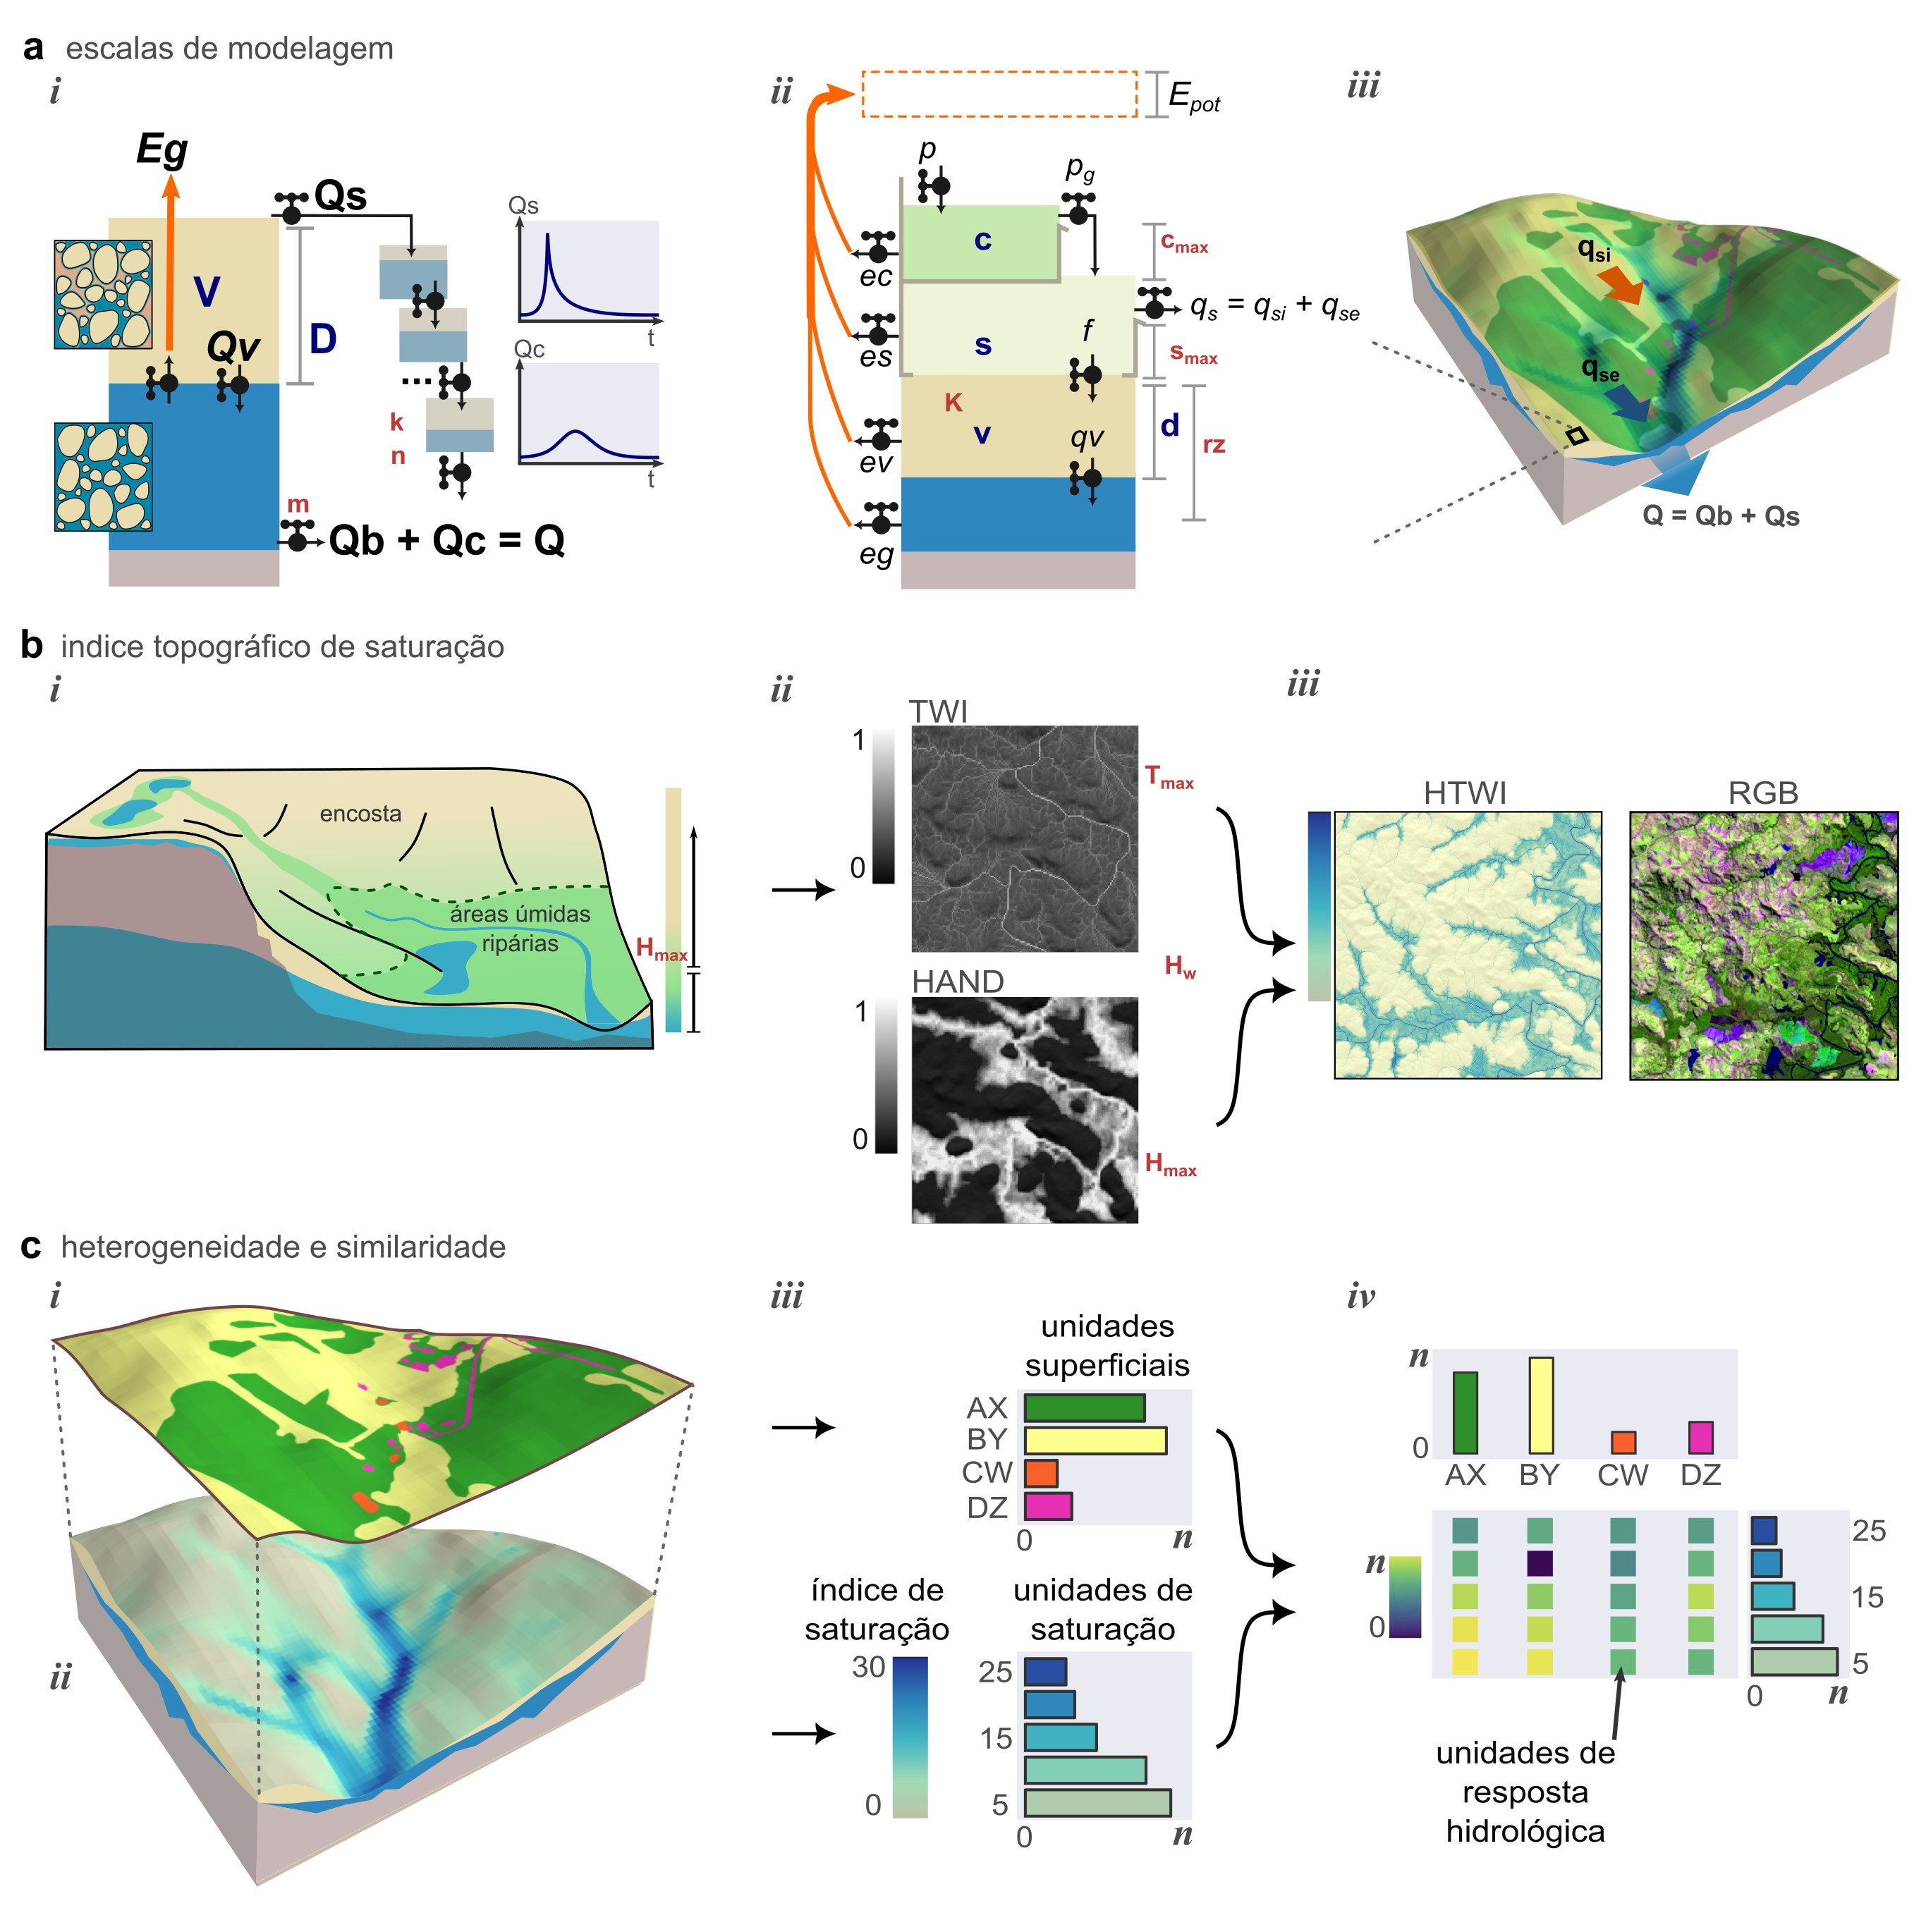
\includegraphics[width=0.98\linewidth]{figs/fig_plans.jpg}		
\caption[O \gls{model} \texttt{PLANS}]
{\textbf{---\;O \gls{model} \texttt{PLANS}.} O \gls{model} consiste em uma versão do \texttt{TOPMODEL} feita sob medida para endereçar o problema da expansão de Soluções Baseadas na Natureza.\;\textbf{a}\;---\;Escalas de modelagem do \gls{model}: \gls{glob-scale} (detalhe \textrm{\textit{i}}); escala das \gls{urh} (detalhe \textrm{\textit{ii}}), e; escala loca, no elemento de malha (detalhe \textrm{\textit{iii}}).\;\textbf{b}\;---\;Índice topográfico de saturação HTWI. O \gls{tsi} parte da \gls{hipotese} de separação dual entre áreas de encosta e áreas ripárias (detalhe \textrm{\textit{i}}). Os índices TWI e HAND são normalizados por lógica \textit{fuzzy} (detalhe \textrm{\textit{ii}}). Uma ponderação entre os índices gera o HTWI (detalhe \textrm{\textit{iii}}).\;\textbf{c}\;---\;Heterogeneidade e similaridade espacial: a camada superficial de variáveis estáticas é separada da camada subterrânea de variáveis dinâmicas (detalhe \textrm{\textit{i}} e \textrm{\textit{ii}}); as variáveis na \gls{loc-scale} são agrupadas em unidades superficiais e unidades de saturação (detalhe \textrm{\textit{iii}}); um histograma bidimensional, ou matriz de frequências, é computado para armazenar as \gls{urh} (detalhe \textrm{\textit{iv}}).
}
\label{fig:hydro:plans} 		
\end{figure}

\par No \gls{model} \texttt{PLANS}, assim como no \texttt{TOPMODEL}, a distribuição local do déficit de água no solo é feita pela função de \gls{downscaling}, definida na Equação \ref{eq:topmodel:d5}, usando um índice topográfico de saturação $\lambda_{i}$ como co-variável. Porém, ao contrário do \texttt{TOPMODEL}, a única \gls{hipotese} fundamentalmente defendida pelo \gls{model} nesse aspecto é a relação linear que a \gls{scaling-func} implica, fato que possibilita o teste de outros índices topográficos para além do \acrshort{atwi} (Figura \ref{fig:hydro:plans}\textbf{b}). Esse relaxamento das hipóteses do \gls{model} clássico foi motivado principalmente pela necessidade prática de endereçar o problema da expansão de \acrshort{nbs} no Brasil, país com uma ampla heterogeneidade de solos e paisagens, incluindo solos tropicais muito mais profundos do que aqueles observados em climas temperados ou subtropicais. Outra motivação, de natureza conceitual, se alicerça sobre as observações empíricas trazidas por Crave \& Gascuel-Odoux (1997) \cite{Crave1997a} a respeito da distribuição das áreas saturadas em uma pequena bacia hidrográfica na França (1,3 km²), com solos variando entre 40 cm a 2 metros de profundidade. No estudo, os autores reportam uma correlação fraca entre a saturação do solo local e o \acrshort{atwi}, além da relativa imobilidade da mancha de saturação no fundo do vale, refutando em grande medida a \gls{teoria} subjacente ao \texttt{TOPMODEL}. Por outro lado, eles mostram que a saturação do solo nos pontos amostrados $i$ possui uma relação inversa com a \textit{diferença de altitude} $\Delta Z_{i, o}$, ou altura $\text{H}_{i, o}$, em relação ao afloramento de água mais próximo $o$. Essa relação inversa se mantém até um dado limiar de altura $\text{H}_\text{max}$, onde então a saturação exibe uma faixa de valores relativamente uniforme. Diante dessas observações, os autores sugerem que nas bacias com solos relativamente profundos e bem drenados a paisagem divide-se em duas partes: a região de cabeceira, mais seca, e a região ripária, mais úmida (Figura \ref{fig:hydro:plans}\textbf{b}, detalhe \textit{i}). Mantidas as outras variáveis constantes, a separação entre essas duas regiões é razoavelmente delimitada pelo limiar de altura $\text{H}_\text{max}$ sobre o fundo do vale. 

% -- figura do Crave?

\par Esse mesmo indicador topográfico de saturação, denominado de \textbf{\gls{hand}}\footnote{A sigla HAND deriva de \say{Height Above the Nearest Drainage}.}, foi articulado dez anos mais tarde por Rennó et \textit{al.} (2008) \cite{Renno2008a}, que demonstram a sua efetividade em mapear áreas úmidas na Amazônia. Mas o diferencial do estudo de Rennó et \textit{al.} (2008) é que os autores organizam o método computacional para se obter o \acrshort{ahand} pela aplicação de técnicas de geoprocessamento de \acrshort{adem}. Em linhas gerais, a técnica consiste em inicialmente se estabelecer um mapa da rede de drenagem, o que pode ser feito por um limiar de iniciação da drenagem $H_{\alpha}\;[\text{L}^2]$, que é a área mínima para o afloramento de água no solo. Com isso, para cada elemento de malha $o$ na rede de drenagem são obtidas as suas respectivas altitudes $Z_{o, i}$ e áreas de drenagens (bacias). Por fim, calcula-se o \acrshort{ahand} local $\text{H}_i$ na área de cada bacia pela diferença entre a altitude local $Z_{i}$ e a altitude da drenagem mais próxima $Z_{o, i}$. O resultado, portanto, é um \acrlong{adem} normalizado para que a altitude nula seja sempre o nível do rio, riacho ou fundo de vale hidrologicamente mais próximo. A derivação do \acrshort{ahand} por geoprocessamento trouxe novas aplicações, como o mapeamento de risco de inundação de grandes rios, pois quanto mais alto se está acima da calha de um rio, maior é a segurança \cite{Nobre2016a}. Fica evidente, porém, que o valor do \acrshort{ahand} é altamente sensível ao mapa de drenagem ou limiar de área $H_{\alpha}$ estabelecido inicialmente, sendo aplicações para o mapeamento de inundações de grandes rios (macro-drenagem) muito diferentes do mapeamento da saturação do solo (micro-drenagem).

\par Assim, a abordagem adotada no \gls{model} \texttt{PLANS} encoraja que o índice topográfico de saturação $\lambda_i$ seja obtido por combinações de lógica \textit{fuzzy} entre o \acrshort{atwi} e o \acrshort{ahand}, fato que resulta no índice \textit{HAND-enhanced TWI}, ou \acrshort{atwi} realçado pelo \acrshort{ahand} (\texttt{HTWI}), ilustrado no detalhe \textit{iii} da Figura \ref{fig:hydro:plans}\textbf{b}. Essa abordagem, na verdade, foi sugerida tangencialmente por Quinn et \textit{al.} (1991) \cite{Quinn1991b} para diferenciar as regiões de drenagem efêmera e perene, mas em relação a diferentes métodos de acúmulo de fluxo. O índice proposto, nessa linha, preserva a característica do \acrshort{atwi} em aumentar a saturação da paisagem de montante para jusante, mas torna esse efeito relativamente mais pronunciado nas proximidades das \gls{sat_areas} do que nas encostas mais secas. O mapa é calculado inicialmente pela normalização \textit{fuzzy} de ambas as variáveis, sendo necessário estabelecer limiares superiores para cada uma delas (Figura \ref{fig:hydro:plans}\textbf{b}, detalhe \textit{ii}). No caso do \acrshort{atwi}, a normalização é ascendente: 
\begin{linenomath*}
\begin{equation}
\label{eq:plans:ftwi}
\tilde{\text{T}}_i = \texttt{MIN}(\text{T}_i/\text{T}_\text{max},\; 1) \quad \forall \; i
\end{equation}
\end{linenomath*}
Em que  $\text{T}_i\;[-]$ é o \acrshort{atwi} local; $\text{T}_\text{max}\;[-]$ é o limiar superior do \acrshort{atwi}, e; $\tilde{\text{T}}_i\in \{0,1\}\;[-]$ é o \acrshort{atwi} local normalizado. No caso do \acrshort{ahand}, a normalização é descendente:
\begin{linenomath*}
\begin{equation}
\label{eq:plans:ftwi}
\tilde{\text{H}}_i = \texttt{MAX}(1 - \text{H}_i/\text{H}_\text{max},\; 0) \quad \forall \; i
\end{equation}
\end{linenomath*}
Em que  $\text{H}_i\;[-]$ é o \acrshort{ahand} local; $\text{H}_\text{max}\;[-]$ é o limiar superior do \acrshort{ahand}, e; $\tilde{\text{H}}_i\in \{0,1\}\;[-]$ é o \acrshort{ahand} local normalizado. Com isso, o \texttt{HTWI} é determinado pela média ponderada entre essas variáveis normalizadas e escalonada de volta para a amplitude original do \acrshort{atwi}:
\begin{linenomath*}
\begin{equation}
\label{eq:plans:htwi}
\text{HT}_{i} = \text{T}_\text{max} \frac{\tilde{\text{T}}_i + H_w \tilde{\text{H}}_i}{1 + H_w} \quad \forall \; i
\end{equation}
\end{linenomath*}
Em que $\text{HT}_{i}\in \{0,\text{T}_\text{max}\}\;[-]$ é o \texttt{HTWI}, e; $H_w\;[-]$ é um fator ou peso adimensional positivo que reflete a dominância do \acrshort{ahand} sobre o \acrshort{atwi}. A \gls{teoria} embutida na derivação do \texttt{HTWI} é que existe um espectro de paisagens hidrológicas que se estende desde a prevalência total de solos rasos e áreas saturadas dinâmicas (dominância total do \acrshort{atwi} sobre o \acrshort{ahand}) até a prevalência total de solos profundos e áreas saturadas estáticas (dominância total do \acrshort{ahand} sobre o \acrshort{atwi}), com alternativas intermediárias entre essas situações extremas. A dominância de um sobre outro é regulada pelo peso $H_w$, enquanto que a mobilidade das áreas saturadas é regulada pelos limiares $\text{T}_\text{max}$ e $\text{H}_\text{max}$. No caso especial em que $H_w = 0$, o \texttt{HTWI} é idêntico ao \acrshort{atwi} truncado em $\text{T}_\text{max}$. Esse índice topográfico de saturação generalizado, ajustável para qualquer paisagem, introduz três \gls{parameters} adicionais no modelo\footnote{Na verdade, ao considerar o limiar de área de drenagem $\text{H}_{\alpha}$ para definição do \acrshort{ahand}, são quatro \gls{parameters} adicionais}, um custo epistemológico que foi considerando aceitável pelos autores diante da necessidade prática de modelar processos hidrológicos nos ambientes diversos do Brasil. Um caminho para se reduzir incertezas na distribuição posterior dos \gls{parameters} talvez seja pré-condicionar a distribuição \textit{anterior} com outras variáveis espaciais obtidas por sensoriamento remoto, como o índices de umidade, a temperatura superficial ou simplesmente a reflectância no infravermelho de ondas curtas, como ilustrado na Figura \ref{fig:hydro:topo}\textbf{a}.

\par A outra diferença do \gls{model} \texttt{PLANS} em relação ao \texttt{TOPMODEL} é a representação da heterogeneidade superficial (Figura \ref{fig:hydro:plans}\textbf{c}). A versão clássica do \texttt{TOPMODEL} foi desenvolvida assumindo-se que a superfície é homogênea, o que faz sentido na bacia hidrográfica de Crimple Beck, na Inglaterra, uma região rural dominada por pastagens para pecuária. Porém, um \gls{model} projetado para endereçar o problema da expansão das SBN deve não somente representar o solo e sua cobertura em situações heterogêneas mas também possibilitar a simulação de cenários de coberturas alternativos, de maneira a se avaliar o impacto positivo ou negativo de uma dada política de expansão. Por exemplo, o \gls{model} deve ser capaz de informar se há diferença no comportamento do \gls{system} hidrológico entre o reflorestamento em diferentes partes da paisagem. Esse requisito é reconhecido por Gao et \textit{al.} (2015) \cite{Gao2015a}, fato que os motivou a implementar uma versão distribuída do \texttt{TOPMODEL} para avaliar impactos hidrológicos da mudança no uso e cobertura da terra. O \gls{model} \texttt{PLANS}, alternativamente, faz uso da abordagem semi-distribuída, colapsando a \gls{loc-scale} em uma escala intermediária de \gls{urh} (Figura \ref{fig:hydro:plans}\textbf{a}, detalhe \textit{ii}). Esse processo é realizado pela tabulação cruzada de unidades superficiais (manchas similares de solos e vegetação) com unidades de saturação (intervalos regulares do índice topográfico de saturação)\footnote{Ainda que os mapas de solos e vegetação sejam mantidos como \gls{input-data} do \gls{model}, aqui cabe ressaltar que esses mapas também são resultado de um processo de \gls{scalab} de outras variáveis locais. Por exemplo, as classes de vegetação e uso da terra fornecidas nos mapas anuais divulgados por Souza et \textit{al.} (2020) \cite{Souza2020a}, utilizadas no \gls{model} \texttt{PLANS}, foram derivadas de agrupamentos da reflectância espectral e índices de bandas de cenas orbitais com auxílio de aprendizado de máquina.} (Figura \ref{fig:hydro:plans}\textbf{c}, detalhes \textit{i} , \textit{ii} e \textit{iii}). Essa tabulação resulta, enfim, em um histograma bidimensional, ou \textbf{matriz de frequências}, que especifica a prevalência em área de cada unidade de \gls{hydro-response} na região espacial de interesse\footnote{A propagação do escoamento para uma dada seção de rio, assim, deve ser feita ao se especificar a prevalência de cada unidade de resposta na área da bacia de interesse, que pode ou não se aproximar da prevalência da região total. Essa abordagem, portanto, permite se avaliar o escoamento final em múltiplas bacia de interesse.}. Como ilustrado no detalhe \textit{iv} da Figura \ref{fig:hydro:plans}\textbf{c}, as colunas expressam o histograma do \gls{tsi} em cada unidade superficial. As linhas da matriz, por outro lado, são similares em termos de saturação, o que facilita prontamente a determinação do décifit local pela função de \gls{downscaling} do \gls{model}. 

\section{Conectividade}

\par Durante este capítulo, eu organizei as reviravoltas correntes na \gls{hydrology} desde a Década Hidrológica Internacional, isto é, dos anos 1960 em diante. Por um lado, na frente experimental, a \gls{age_inf} enfrentou sua crise derradeira com a ascensão de um novo \gls{paradigma} que reafirma a diferenciação e singularidade dos mecanismos de \gls{hydro-response} como função do clima, topografia, solos, vegetação, etc. Por outro, no âmbito da modelagem, o advento dos computadores digitais abriu caminho para métodos ontologicamente diversos, como a \gls{sys-dyn}, campos vetoriais e modelos estatísticos, sendo os dois primeiros baseados na descrição teórica de processos e o último exclusivamente baseado em dados obtidos empiricamente.

% figure
\begin{figure}[t!] 
\centering				
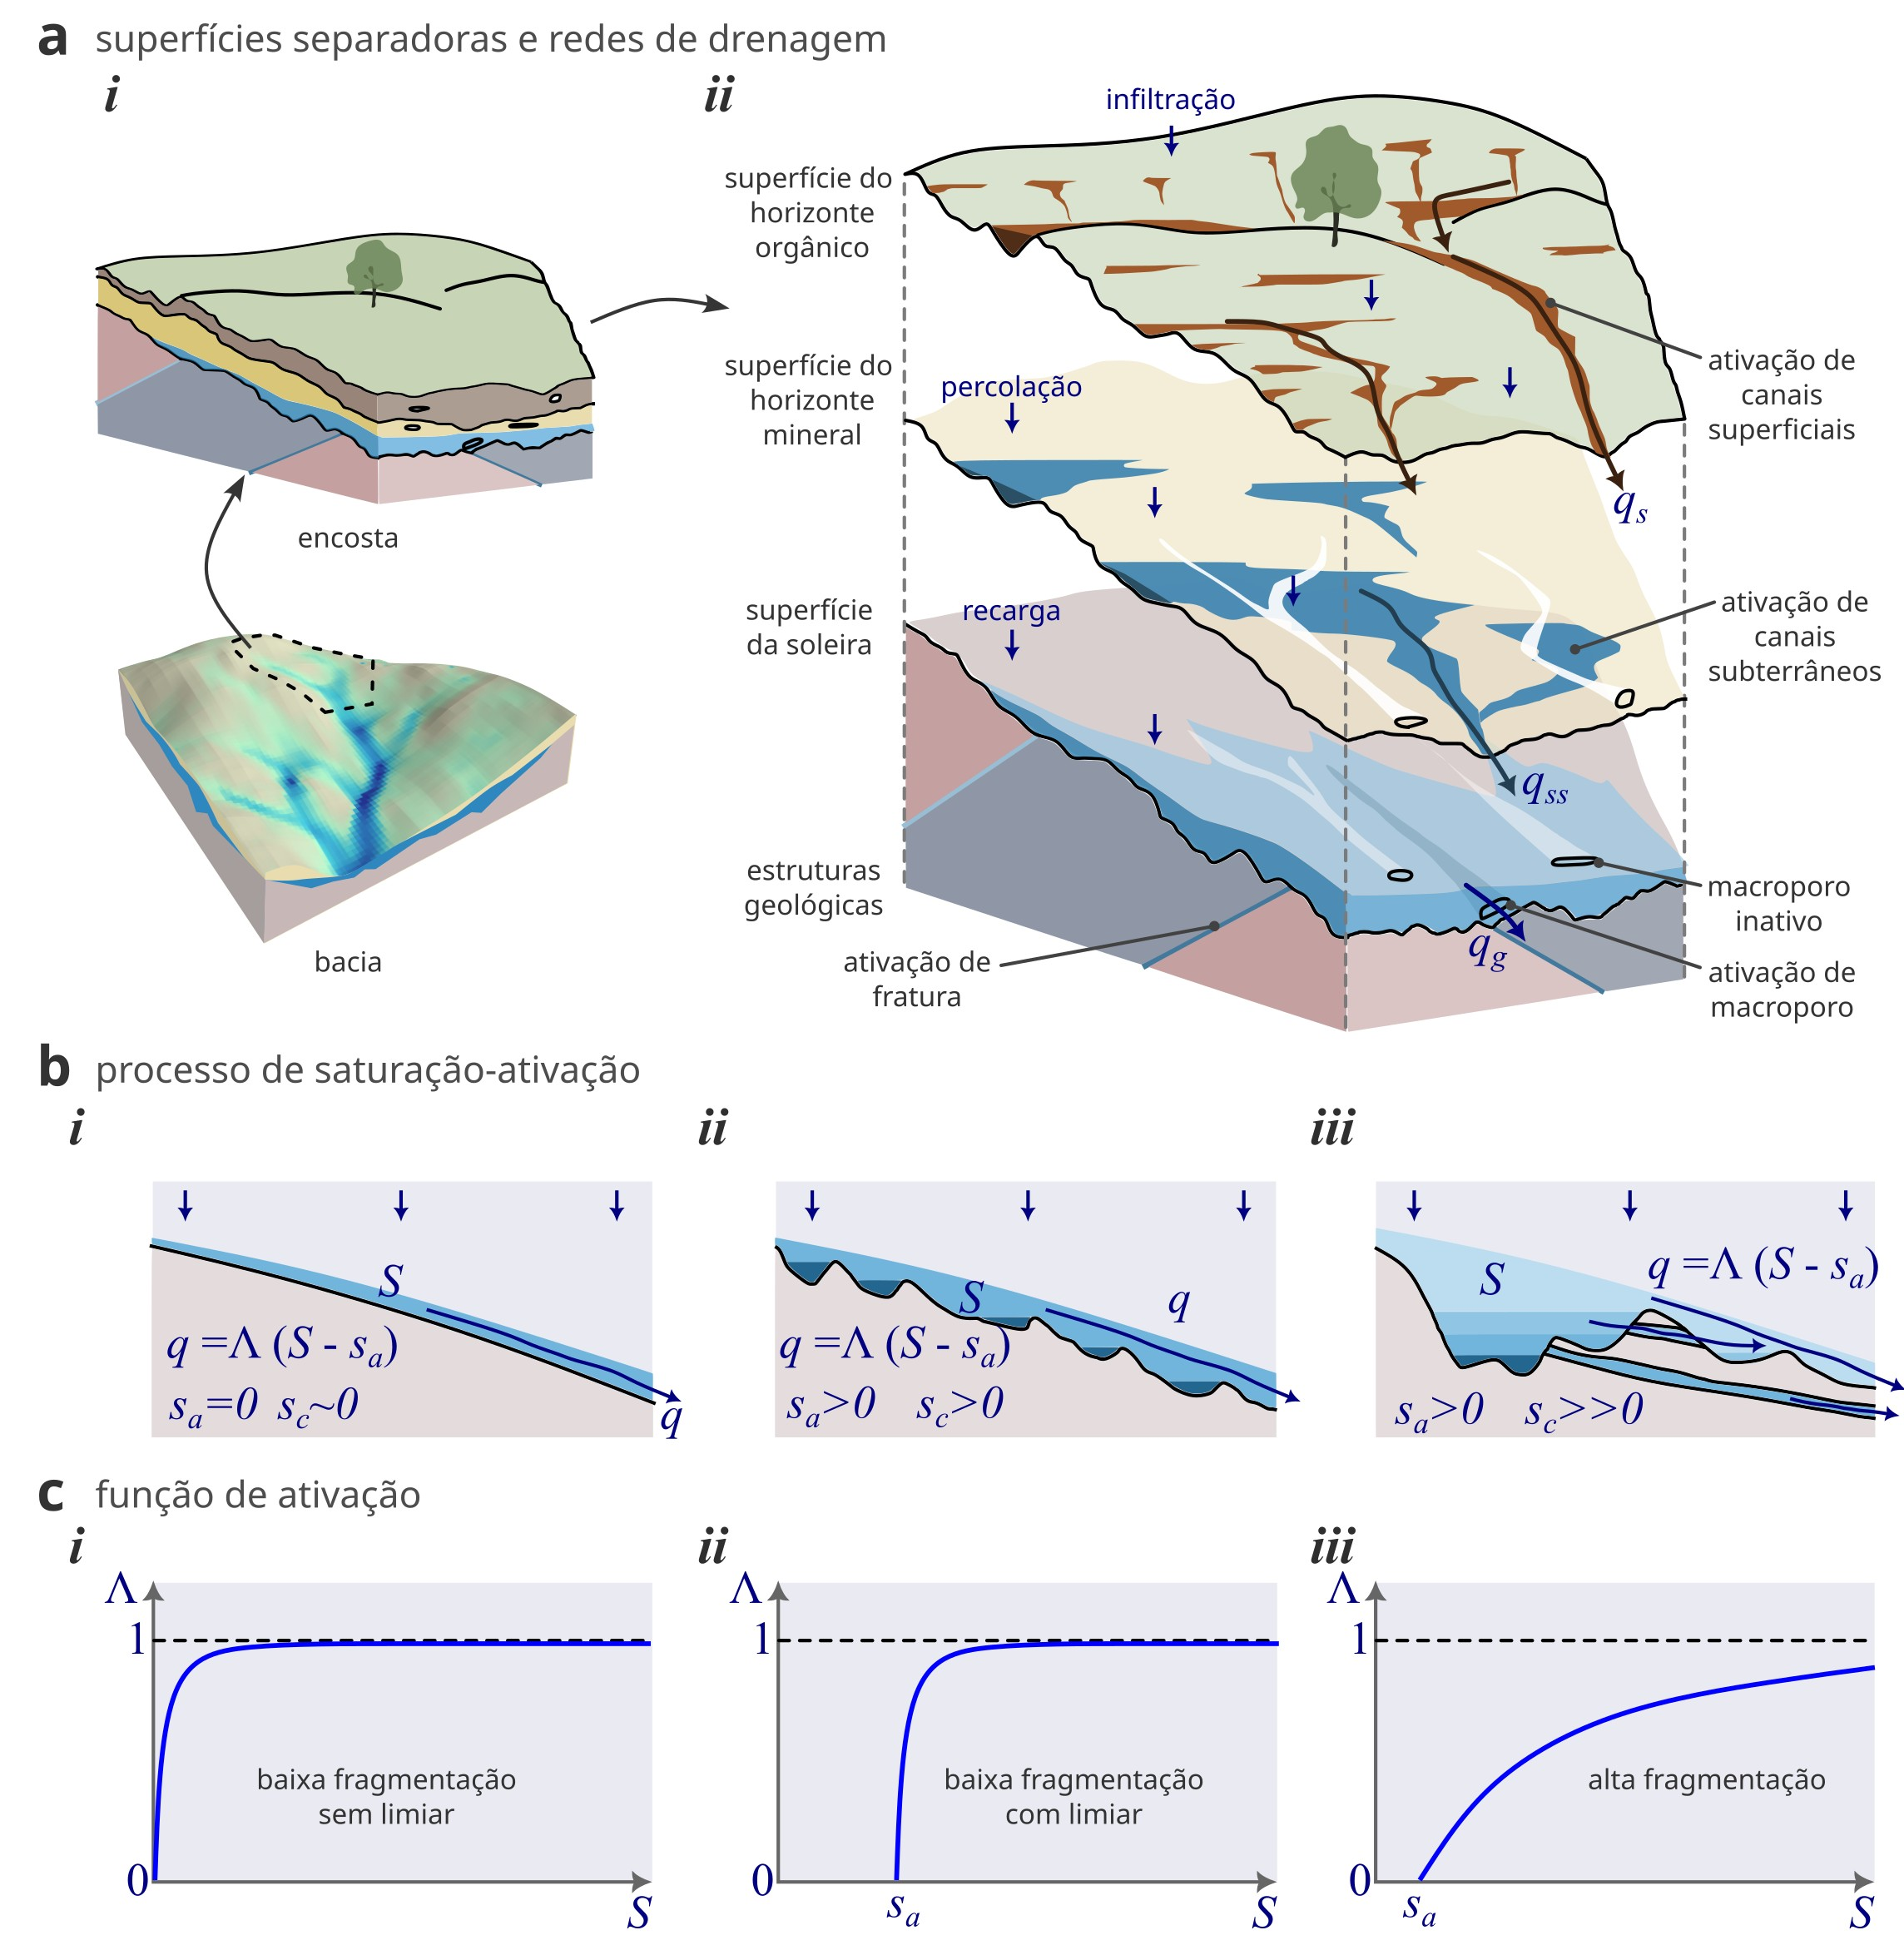
\includegraphics[width=0.98\linewidth]{figs/fig_connect.jpg}		
\caption[O \gls{paradigma} da conectividade]
{\textbf{---\;O \gls{paradigma} da conectividade.} A \gls{conect-theory} proposta por Jeffrey McDonnell e colegas apresenta um potencial unificador e revolucionário na \gls{hydrology}.\;\textbf{a}\;---\;O \gls{percept-model} parte do princípio de que todas as respostas hidrológicas são consequência de um mesmo fenômeno. As \gls{perm_trans} vertical criam \gls{sepsurf}. Assim, a rede de canais nessas superfícies pode ser eventualmente saturada e ativada. Interações ocorrem também de baixo para cima, quando uma camada satura-se o suficiente para interferir no processo de percolação da camada imediatamente acima.\;\textbf{b}\;---\;O \gls{fillspill} ocorre em razão da topologia da rede de canais que drenam a superfície separadora em diversas escalas aninhadas. A superfície pode ser totalmente conectada (detalhe \textrm{\textit{i}})) ou demandar um \gls{activ-level} inicial $s_a$ (detalhe \textrm{\textit{ii}}). Uma superfície com alta fragmentação $s_c$ oferece múltiplas redes de drenagem ativadas incrementalmente, atenuando o sinal da resposta (detalhe \textrm{\textit{iii}}).\;\textbf{c}\;---\;A \gls{func-activ} $\Lambda$ pode ser modelada em termos de um processo de saturação que tende ao \gls{flux-max} potencial $S - s_a$ à medida que a superfície satura-se, ou seja, $\Lambda \rightarrow 1$.    
}
\label{fig:connnect} 		
\end{figure}

\par Como novos paradigmas científicos não se estabelecem por serem perfeitos, mas por serem melhores que a concorrência, ambas as abordagens que se instalaram no campo não estão livres de problemáticas. No caso das pesquisas experimentais, o \gls{paradigma} da diferenciação encontrou paradoxos empíricos envolvendo a rápida mobilização da água velha e a diversidade de assinaturas geoquímicas, dificilmente explicáveis pelos mecanismos articulados pela sistematização de Dunne (1983) \cite{Dunne1983}. Além disso, o programa de pesquisa experimental resume-se a catalogar os mecanismos de \gls{hydro-response} de cada bacia singular. Ainda que o catálogo possa ser detalhado e expandindo eternamente, esse modo operacional não contribui para uma \gls{teoria} científica unificadora \cite{Mcdonnell2003a}. No caso da modelagem, crises se abateram sobre as diferentes abordagens, fazendo surgir os dois principais problemas epistemológicos inescapáveis da modelagem hidrológica: o problema de equifinalidade e o \gls{scale_problem} \cite{Beven1996a}. Ainda que diferentes, os problemas são interconectados, resultando em incertezas epistêmicas inexoráveis que pairam sobre os resultados dos modelos. O imperativo desses problemas epistêmicos, ao mesmo tempo que eclipsou a abordagem de campos vetoriais (obrigando seus proponentes a apelar para vantagens pragmáticas), trouxe uma nova luz sobre a ontologia da \gls{sys-dyn}, fazendo-a útil para se estimar as incertezas pela aplicação de \gls{models-semid} de baixo custo computacional.

\par Dito isso, encerrarei o capítulo articulando as recentes ideias revolucionárias de Jeffrey McDonnell e demais colegas, que nas últimas duas décadas buscaram pavimentar o caminho para um novo \gls{paradigma} unificador na \gls{hydrology}. Essas ideias possuem um impacto direto sobre a aplicação de modelos hidrológicos no contexto de bacias de ordem zero, sendo de primeira importância a sua assimilação e articulação em próximas versões do \gls{model} \texttt{PLANS}. Ainda que amplamente publicada, a síntese de McDonnell pode ser rastreada em três artigos separados por intervalos de aproximadamente dez anos: McDonnell (2003) \cite{Mcdonnell2003a}; McDonnell (2013) \cite{Mcdonnell2013}, e; McDonnell et \textit{al.} (2021) \cite{mcdonnell2021}.

\par Inicialmente, McDonnell (2003) demonstra o descolamento crescente entre modelos hidrológicos e evidências, salientando que os mecanismos da Década Hidrológica Internacional fundamentam-se em premissas que falham em explicar o \gls{old_water_paradox}. Em essência, ele argumenta que as evidências apontam tanto para uma maior separação entre as encostas bem drenadas e as \gls{sat_areas} quanto para uma maior influência da \gls{bedrock_topo} no afloramento da água subterrânea. Juntos, esses dois fatores produzem escoamento translacional rápido de água pré-evento (velha) com assinaturas geoquímicas diversas. No campo da modelagem, McDonnell (2003) sustenta que a ontologia apropriada para os novos desafios é a \gls{sys-dyn}, não por mera conveniência, mas por permitir a representação dos diferentes compartimentos da \gls{zero-basin}, principalmente encostas e zonas ripárias, e por garantir experimentos exploratórios a um baixo custo computacional. Como destacado na epígrafe do capítulo, a \gls{sys-dyn} se reafirma como um \gls{paradigma} ontológico ao mesmo tempo intuitivo e objetivo para se compreender e aprender sobre sistemas ambientais.

\par O segundo passo de McDonnell (2013) é propor a \textbf{\gls{conect-theory}} como explicação definitiva tanto dos processos hidrológicos sistematizados por Dunne (1983) quanto das (não tão) recentes descobertas sobre o \gls{old_water_paradox}. Inicialmente reportada em Meerveld \& McDonnell (2006) \cite{Meerveld2006b} para explicar processos em uma bacia experimental específica, McDonnell generaliza seus conceitos, tratando-a como uma \gls{teoria} revolucionária e unificadora que busca resolver a crise instaurada no campo. McDonnell propõe essa \gls{teoria} a partir de uma pergunta que soa como heresia: seriam as respostas rápidas e lentas das bacias todas \textit{o mesmo fenômeno}?

\begin{adjustwidth}{100pt}{0pt}
\medskip
\small (...) a simples premissa de que todos os processos de escoamento são o mesmo abre novas trilhas a serem exploradas: será que existe um comportamento emergente comum entre todos os tipos de escoamento?\footnote{Tradução livre de: \textit{the simple premise that all runoff processes are the same opens up new avenues to explore: Is there common emergent behaviour across all runoff types?}} -- Jeffrey McDonnell (2013, p. 4110) \cite{Mcdonnell2013}.
\medskip
\end{adjustwidth}

Essa pergunta provocativa leva-o a demonstrar que qualquer \gls{system} formado por redes de pequenos canais pode ser modelado pela \textbf{Teoria da Percolação}, uma ramificação matemática da Teoria das Redes\footnote{Ao contrário de teorias científicas, que precisam de evidências empíricas para serem corroboradas, as teorias matemáticas fundamentam-se em axiomas e \gls{infer-dedu}.} \cite{Janzen2015a}. De acordo com essa \gls{teoria}, o fluxo ocorre através de uma rede à medida que existem conexões entre os nós. No caso de uma \gls{zero-basin}, no mundo físico, as diferentes partes do \gls{system} funcionam cada uma como uma rede de pequenos reservatórios conectados por pequenos canais (abertos ou fechados, macroscópicos ou microscópicos). Aqui, surge a relevância de dois conceitos-chave da \gls{teoria}: (1) a \textbf{\gls{sepsurf}} entre os compartimentos, criada pela transição de permeabilidade vertical entre os horizontes do solo, e; (2) o \textbf{\gls{activ-threshold}} do compartimento, que decorre principalmente da heterogeneidade da superfície separadora.

\par Um exemplo bem claro disso consiste na geração das enxurradas, quando a capacidade infiltração do solo é insuficiente. Tipicamente, o nível das depressões superficiais precisa atingir um \gls{activ-threshold}, quando algumas depressões superficiais se conectam pela primeira vez e passam a derramar água morro abaixo. Com mais tempo de chuva, as poças de água passam a se colmatar cada vez mais, até um momento em que toda água da chuva incidente pode escoar morro abaixo. A velocidade que a conexão acontece depende da heterogeneidade da superfície do solo: uma superfície lisa é muito mais conectada que uma superfície rugosa.

\par Apesar de óbvio, McDonnell sugere que o \textbf{\gls{fillspill}}\footnote{Tradução livre do inglês \textit{fill and spill}.} que gera as enxurradas ocorre em todas as camadas subterrâneas onde o fluxo vertical de água esbarra em uma transição de permeabilidade, incluindo a soleira de rocha relativamente impermeável (Figura \ref{fig:connnect}\textbf{a}). A única diferença do ambiente subterrâneo é que a rede de canais é composta pelos micro e macroporos do horizonte imediatamente superior. Nesse contexto, a \gls{teoria} permite inclusive que quantidades relativamente pequenas da água do evento (água nova) ativem a conexão entre bolsões de água armazenada antes do evento (água velha). A pressurização na zona saturada, assim como a formação de sifões naturais no subsolo, eventualmente expulsam \textit{mais} água do que entrou, gerando um balanço de massa negativo na encosta e um comportamento histerético dos pulsos de vazão. Por fim, quando uma superfície separadora satura-se o suficiente, passa a propagar esse efeito de baixo para cima, causando a saturação da camada superior, originando dessa forma condições análogas às \gls{sat_areas} que observamos na superfície.

\par Por fim, no seu terceiro movimento, McDonnell et \textit{al.} (2021) articulam como abordar a \gls{conect-theory} no contexto da modelagem, considerando o \gls{scale_problem}. Novamente, a \gls{sys-dyn} é apresentada como a ontologia adequada para a representação do \gls{sys-target}, com ênfase na definição explícita da escala de interesse, identificando os processos de saturação-ativação que se manifestam na \gls{model-scale} escolhida. A \gls{hipotese} dos autores é que processos de saturação-ativação ocorrem em todas as escalas, porém o sinal emitido pelas escalas menores são progressivamente mascarados pela saturação-ativação nas escalas maiores (Figura \ref{fig:connnect}\textbf{b}). Por exemplo, enquanto na escala das bacias de ordem zero o \gls{fillspill} é ditado principalmente pela topografia, solo e vegetação, esse sinal se apaga na escala de bacias de ordem superior, tornando-se mais dominantes os efeitos de saturação-ativação do \gls{system} de drenagem dos rios e inundação das planícies. Assim, as pesquisas experimentais e de modelagem devem questionar explicitamente qual é a escala abordada e quais são os processos de saturação-ativação críticos para compreender o \gls{sys-target}. Modelos de \gls{sys-dyn} relativamente simples (mas objetivos) podem capturar esse conhecimento, formalizando a \gls{hipotese} principal do \textbf{\gls{func-activ}}, que assume a seguinte forma geral:
\begin{linenomath*}
\begin{equation}
\label{eq:conect:general}
Q_a = 
\begin{cases} 
    0 & \text{se } \quad S \leq s_a\\
    \Lambda \cdot (S - s_a) & \text{se } \quad S > s_a
\end{cases}
\end{equation}
\end{linenomath*}
Em que $Q_a\;[\text{L}\text{T}^{-1}]$ é o fluxo de ativação do reservatório com nível $S\;[\text{L}]$; $s_{a}\;[\text{L}]$ é o \textbf{\gls{activ-level}} do reservatório, e; $\Lambda \;[\text{T}^{-1}]$ é a \textbf{\gls{func-activ}} do reservatório, a ser definida com base nas \gls{aux-hyp} do \gls{model}. No capítulo anterior, durante o desenvolvimento do protótipo de \gls{model} hidrológico, eu apliquei esses exatos princípios para o fluxo de resposta rápida $R$ do reservatório superficial $S_1$ (ver Seção \ref{sec:systems:model}). A Equação \eqref{eq:fast_response} possui exatamente a mesma estrutura que a Equação \eqref{eq:conect:general}, sendo $\Lambda = c$, um coeficiente de escoamento definido entre 0 e 1 e obtido por uma \gls{func-activ} com a seguinte estrutura (Figura \ref{fig:connnect}\textbf{c}):
\begin{linenomath*}
\begin{equation} 
	\label{eq:conect:af}
	\Lambda = \frac{(S - s_a)}{(S - s_a) + s_c} \frac{1}{\Delta t}
\end{equation}
\end{linenomath*}
Em que $s_{a}\;[\text{L}]$ é o \gls{activ-level} do reservatório, e;  $s_{c}\;[\text{L}]$ é o \textbf{\gls{frag-level}} do reservatório. Essa função, ao ser acoplada em \eqref{eq:conect:general}, implica que o fluxo de saída $Q_a$ causado pela ativação tende assintoticamente para o \gls{flux-max} potencial ($S - s_a$) à medida que o nível $S$ do reservatório aumenta, pois níveis maiores ativam cada vez mais a rede de drenagem. Ou seja, $\lim _{S \to \infty} \Lambda= 1$ em \eqref{eq:conect:af} e $\lim _{S \to \infty} Q_a = (S - s_a)/ \Delta t$ em \eqref{eq:conect:general}. O \gls{frag-level} $s_c$ é um parâmetro que exerce o papel de regular a velocidade desse processo, sendo uma medida de conectividade inversa (quanto maior, menos conectado é o reservatório). A interpretação física do \gls{frag-level} consiste no nível $S$ necessário para se atingir metade do \gls{flux-max} potencial. A \textbf{equação de Michaelis-Menten} \cite{Johnson2011a}, que descreve um processo de saturação de enzimas, não por acaso apresenta estrutura idêntica, sendo uma \gls{homology} notável. Outra estrutura idêntica é a equação do \textbf{método \acrshort{cn}}, proposta empiricamente partir dos resultados de Mockus (1949) \cite{mockus1949}. A diferença, nesse caso, é que os criadores do método \acrshort{cn} expressam o nível $S$ em termos de chuva acumulada $P$, o que somente é válido para um reservatório superficial com capacidade ilimitada. O \gls{frag-level}, nessa linha, é expresso em termos de um coeficiente de conectividade adimensional, de forma que $s_c = (1000/\text{CN}) - 10$. Tais homologias e explicações teóricas de velhos ajustes empíricos definem os contornos de uma \gls{teoria} científica legitimamente revolucionária. $\blacksquare$

\clearpage

\section{Resumo do capítulo} \label{sec:hydro:summary}

\par Neste capítulo, ofereci uma visão histórica e teórica sobre a evolução dos modelos hidrológicos, destacando as principais mudanças nas abordagens e paradigmas científicos. Começando pelas encostas, onde os processos hidrológicos se iniciam, explorei a transição do \gls{model} de infiltração de Horton para concepções mais complexas que incorporam variabilidade climática, geomorfológica e biológica. Analisam-se também as limitações enfrentadas por modelos computacionais modernos, como problemas de escala e equifinalidade, culminando na \gls{conect-theory}, que propõe uma integração inovadora dos processos de escoamento superficial e subterrâneo.

\begin{itemize}
    \item[$\blacksquare$] \textbf{As encostas são onde tudo começa}. As respostas hidrológicas rápidas (enchentes) e lentas (estiagens) iniciam-se com a chuva nas encostas, ou bacias de ordem zero. Simplificar essa complexidade pode gerar modelos inadequados, especialmente no contexto da revitalização de bacias hidrográficas. Portanto, é crucial reconhecer as teorias sobre a geração de escoamento nessa escala
    
    \item[$\blacksquare$] \textbf{A Idade da Infiltração}. Durante meados do século XX, estabeleceu-se a hegemonia do \gls{model} hidrológico de Horton, que explicava as respostas hidrológicas pela capacidade de infiltração do solo, separando a chuva entre enxurradas e recarga. Embora superado, esse \gls{paradigma} elevou a \gls{hydrology} de sua fase empírica para uma geociência.

    \item[$\blacksquare$] \textbf{A Idade da Diferenciação}. Com a Década Hidrológica Internacional, nos anos 1960, surgiram novas evidências e teorias que refutaram Horton. Esse novo \gls{paradigma} explora como respostas hidrológicas diferentes emergem devido ao clima, topografia, solos e vegetação. Além das enxurradas, destacaram-se os papéis dos macroporos e \gls{sat_areas}. No entanto, uma crise surgiu com o \gls{old_water_paradox}.
    
    \item[$\blacksquare$] \textbf{Limitações inevitáveis}. Computadores digitais viabilizaram os modelos hidrológicos, divididos em duas famílias: baseados em dados (predições) e baseados em processos (explicações). A \gls{sys-dyn} expôs as limitações impostas pela equifinalidade e problemas de escala, que se mantiveram mesmo com tentativas de solução usando modelos baseados em campos vetoriais.
    
    \item[$\blacksquare$] \textbf{Escalonamento de informações}. O \gls{scale_problem} refere-se à dificuldade de compatibilizar as escalas naturais dos processos hidrológicos com a observacional e conceitual. A solução é o \gls{scalab} de informações. O \texttt{TOPMODEL} faz isso ao escalonar a saturação do solo com o índice \texttt{TWI}. O \texttt{PLANS} combina \texttt{HAND} e \texttt{TWI} para escalonar a saturação em diferentes paisagens e instanciar \gls{urh}.
    
    \item[$\blacksquare$] \textbf{A Teoria da Conectividade}. Jeffrey McDonnell propõe uma \gls{teoria} unificadora e revolucionária que sugere que escoamentos superficiais e subterrâneos são manifestações de um único fenômeno, a saturação-ativação de redes de canais. Diante das limitações inescapáveis, a \gls{sys-dyn} é eleita a melhor alternativa para modelar essa \gls{teoria}.
    
\end{itemize}

\end{document}